\documentclass[aspectratio=169,10pt]{beamer}

\usepackage[T1]{fontenc}
\usepackage[utf8]{inputenc}
\usepackage{lmodern}
\usepackage{array}
\usepackage{booktabs}
\usepackage{colortbl}
\usepackage{graphicx}
\usepackage{tikz}
\usetikzlibrary{arrows.meta,positioning,shapes.geometric,fit}

% Auto-generated by slides/generate_slide_assets.py
\newcommand{\CurrentAtlasStatus}{validated}
\newcommand{\CurrentAtlasPolicy}{fixed-policy}
\newcommand{\CurrentAtlasRuns}{30}
\newcommand{\CurrentAtlasEstimators}{17}
\newcommand{\CanonicalEstimatorCount}{17}
\newcommand{\ReadinessIssueCount}{0}

\newcommand{\DynamicTopTable}{%
\begin{tabular}{llrrrr}
\toprule
Estimator & Family & Geo. RMSE & Worst & CPU us & Latency ms \\
\midrule
ESPRIT & Window-based & 0.035 & 0.355 & 89 & 8.3 \\
Koopman (RK-DPMU) & Data-driven & 0.04 & 0.432 & 156 & 12.5 \\
TFT & Window-based & 0.054 & 2.952 & 9 & 16.6 \\
IPDFT & Window-based & 0.054 & 0.59 & 9 & 33.3 \\
SOGI-FLL & Loop-based & 0.063 & 0.844 & 8 & 0 \\
ZCD & Loop-based & 0.063 & 0.65 & 5 & 16.7 \\
SOGI-PLL & Loop-based & 0.065 & 0.457 & 9 & 0 \\
\bottomrule
\end{tabular}%
}

\newcommand{\RfeTopTable}{%
\begin{tabular}{llrrrr}
\toprule
Estimator & Family & Geo. RFE & Geo. RMSE & CPU us & Latency ms \\
\midrule
UKF & Model-based & 6.864 & 0.089 & 11 & 0 \\
EKF & Model-based & 7.406 & 0.384 & 9 & 0 \\
TFT & Window-based & 8.842 & 0.054 & 9 & 16.6 \\
SOGI-FLL & Loop-based & 12.017 & 0.063 & 8 & 0 \\
RA-EKF & Model-based & 14.033 & 0.097 & 13 & 0 \\
PI-GRU & Data-driven & 16.293 & 0.07 & 3509 & 9.1 \\
Koopman (RK-DPMU) & Data-driven & 19.046 & 0.04 & 156 & 12.5 \\
\bottomrule
\end{tabular}%
}

\newcommand{\HarmonicsEndpointTable}{%
\begin{tabular}{llrrr}
\toprule
Estimator & Family & 1\% THD & 30\% THD & Ratio 30/1 \\
\midrule
ZCD & Loop-based & 2.69e-04 & 86.37 & 321452 \\
RA-EKF & Model-based & 0.018 & 0.142 & 7.88 \\
TFT & Window-based & 5.03e-03 & 0.151 & 30.00 \\
EKF & Model-based & 1.21e-03 & 2.426 & 2001 \\
SOGI-PLL & Loop-based & 0.030 & 0.226 & 7.46 \\
UKF & Model-based & 3.48e-03 & 2.301 & 661 \\
SOGI-FLL & Loop-based & 0.010 & 0.283 & 28.28 \\
\bottomrule
\end{tabular}%
}

\newcommand{\RegimeDiagnosticTable}{%
\begin{tabular}{lll}
\toprule
Stress & Estimator & Paper-grade pattern \\
\midrule
RoCoF & LKF & 5.5$\times$ worse on down-ramp at $\pm50$ Hz/s \\
RoCoF & TKEO & 3.9$\times$ worse on down-ramp at $\pm50$ Hz/s \\
RoCoF & RLS & 3.1$\times$ worse on down-ramp at $\pm50$ Hz/s \\
RoCoF & EKF/UKF/RA-EKF & approximately sign-symmetric at $\pm50$ Hz/s \\
Magnitude & ZCD & fails deep sag; remains accurate on matching swell \\
Harmonics & ZCD & best at low THD, collapses above $\sim$20\% THD \\
\bottomrule
\end{tabular}%
}


\definecolor{ofbBlue}{HTML}{156082}
\definecolor{ofbRust}{HTML}{E97132}
\definecolor{ofbPlum}{HTML}{6A4C93}
\definecolor{ofbMoss}{HTML}{8A8F2F}
\definecolor{ofbRed}{HTML}{B23A48}
\definecolor{ofbInk}{HTML}{0E2841}
\definecolor{ofbSoft}{HTML}{F3F5F7}
\definecolor{ofbGreen}{HTML}{196B24}
\definecolor{ofbGold}{HTML}{E97132}
\definecolor{ofbViolet}{HTML}{A02B93}
\definecolor{ofbCanvas}{HTML}{FFFFFF}
\definecolor{ofbMuted}{HTML}{5B677A}
\definecolor{ofbLine}{HTML}{D9E1E8}
\definecolor{ofbNavy}{HTML}{0E2841}
\definecolor{sgsmaTeal}{HTML}{12695F}
\definecolor{sgsmaAqua}{HTML}{A8E6DF}
\definecolor{cardFill}{HTML}{F8FAFB}
\definecolor{cardBorder}{HTML}{CBD7DF}
\newcommand{\sgsmaTitleBg}{figures/sgsma_title_bg.png}
\newcommand{\sgsmaDividerBg}{figures/sgsma_divider_bg.png}
\newcommand{\sgsmaContentBg}{figures/sgsma_content_bg.png}

\usetheme{default}
\usecolortheme[named=ofbBlue]{structure}
\setbeamertemplate{navigation symbols}{}
\setbeamercolor{normal text}{fg=ofbInk,bg=ofbCanvas}
\setbeamercolor{title}{fg=white,bg=ofbNavy}
\setbeamercolor{frametitle}{fg=ofbInk,bg=ofbCanvas}
\setbeamercolor{block title}{fg=white,bg=sgsmaTeal}
\setbeamercolor{block body}{fg=ofbInk,bg=cardFill}
\setbeamercolor{footline}{fg=white}
\setbeamerfont{frametitle}{family=\rmfamily,series=\mdseries,size=\fontsize{16.5}{19}\selectfont}
\setbeamerfont{title}{family=\rmfamily,series=\mdseries,size=\Large}
\setbeamerfont{block title}{series=\bfseries,size=\small}
\setbeamersize{text margin left=8mm,text margin right=8mm}
\usebackgroundtemplate{\includegraphics[width=\paperwidth,height=\paperheight]{\sgsmaContentBg}}
\setbeamertemplate{itemize item}{\raisebox{0.15ex}{\scriptsize\textcolor{ofbBlue}{$\bullet$}}}
\setbeamertemplate{itemize subitem}{\raisebox{0.1ex}{\tiny\textcolor{ofbGold}{$\bullet$}}}
\setbeamertemplate{enumerate item}{\textcolor{ofbBlue}{\insertenumlabel.}}
\setbeamertemplate{blocks}[rounded][shadow=false]
\setbeamertemplate{frametitle}{%
  \vspace{0.58cm}
  \hspace{8mm}\begin{minipage}[t]{0.76\paperwidth}
    \raggedright\hyphenpenalty=10000\exhyphenpenalty=10000
    \usebeamerfont{frametitle}\color{ofbInk}\insertframetitle
  \end{minipage}\par
  \vspace{0.05cm}
}
\setbeamertemplate{footline}{%
  \begin{tikzpicture}[remember picture,overlay]
    \node[anchor=south, text=white, font=\tiny] at ([xshift=-0.08\paperwidth,yshift=0.13cm]current page.south) {\insertframenumber/\inserttotalframenumber};
  \end{tikzpicture}%
  \vspace*{0.84cm}%
}

\newcommand{\artifact}[1]{\vspace{0.20em}{\tiny\color{ofbMuted}Source: \texttt{#1}}}
\newcommand{\metric}[2]{\textbf{#1}: #2}
\newcommand{\callout}[1]{%
  \vspace{0.25em}\noindent
  \begin{tikzpicture}
    \node[
      draw=cardBorder,
      fill=cardFill,
      rounded corners=2pt,
      line width=0.45pt,
      inner xsep=7pt,
      inner ysep=6pt,
      text width=0.94\linewidth,
      align=left
    ] {\small #1};
    \draw[sgsmaTeal, line width=1.3pt] ([xshift=0.5pt,yshift=-0.5pt]current bounding box.north west) -- ([xshift=0.5pt,yshift=0.5pt]current bounding box.south west);
  \end{tikzpicture}%
  \vspace{0.15em}
}
\newcommand{\tagpill}[2]{%
  \tikz[baseline=(x.base)]\node[inner xsep=5pt,inner ysep=2pt,rounded corners=2pt,fill=#1!12,draw=#1,text=ofbInk,font=\scriptsize\bfseries] (x) {#2};%
}
\newcommand{\statcard}[3]{%
\begin{tikzpicture}
\node[
  draw=cardBorder,
  fill=cardFill,
  rounded corners=2pt,
  line width=0.55pt,
  inner sep=7pt,
  text width=0.86\linewidth,
  minimum height=1.18cm,
  align=left
] {
{\scriptsize\bfseries\color{ofbMuted}#2}\\[0.10em]
{\Large\bfseries\color{#1}#3}
};
\draw[#1, line width=1.5pt] ([xshift=0.5pt,yshift=-0.5pt]current bounding box.north west) -- ([xshift=0.5pt,yshift=0.5pt]current bounding box.south west);
\end{tikzpicture}}
\newcommand{\atlaspreviewbanner}{%
  \vspace{-0.10cm}%
  \noindent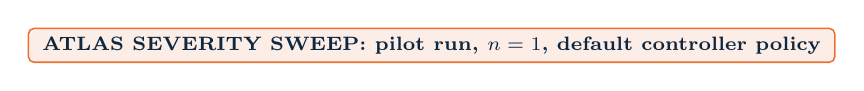
\begin{tikzpicture}
    \node[
      anchor=west,
      rounded corners=2pt,
      fill=ofbRust!12,
      draw=ofbRust,
      line width=0.55pt,
      text=ofbInk,
      font=\scriptsize\bfseries,
      inner xsep=5pt,
      inner ysep=3pt
    ] at (0,0)
    {ATLAS SEVERITY SWEEP: pilot run, $n=1$, default controller policy};
  \end{tikzpicture}\par\vspace{-0.10cm}%
}
\newcommand{\readinessmetricbanner}{%
  \vspace{-0.10cm}%
  \noindent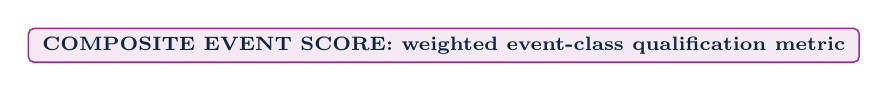
\begin{tikzpicture}
    \node[
      anchor=west,
      rounded corners=2pt,
      fill=ofbViolet!10,
      draw=ofbViolet,
      line width=0.55pt,
      text=ofbInk,
      font=\scriptsize\bfseries,
      inner xsep=5pt,
      inner ysep=3pt
    ] at (0,0)
    {COMPOSITE EVENT SCORE: weighted event-class qualification metric};
  \end{tikzpicture}\par\vspace{-0.10cm}%
}
\newcommand{\extendedresultsbanner}{%
  \vspace{-0.10cm}%
  \noindent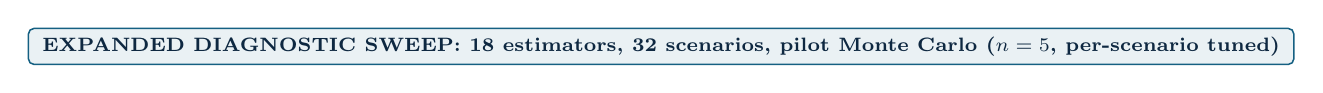
\begin{tikzpicture}
    \node[
      anchor=west,
      rounded corners=2pt,
      fill=ofbBlue!9,
      draw=ofbBlue,
      line width=0.55pt,
      text=ofbInk,
      font=\scriptsize\bfseries,
      inner xsep=5pt,
      inner ysep=3pt
    ] at (0,0)
    {EXPANDED DIAGNOSTIC SWEEP: 18 estimators, 32 scenarios, pilot Monte Carlo ($n=5$, per-scenario tuned)};
  \end{tikzpicture}\par\vspace{-0.10cm}%
}
\newcommand{\diagbanner}{%
  \vspace{-0.10cm}%
  \noindent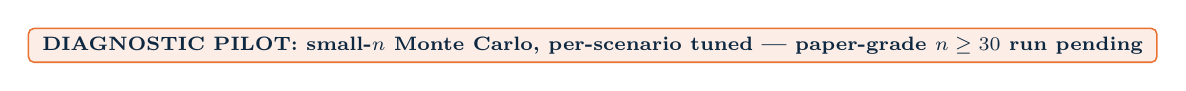
\begin{tikzpicture}
    \node[
      anchor=west,
      rounded corners=2pt,
      fill=ofbRust!12,
      draw=ofbRust,
      line width=0.55pt,
      text=ofbInk,
      font=\scriptsize\bfseries,
      inner xsep=5pt,
      inner ysep=3pt
    ] at (0,0)
    {DIAGNOSTIC PILOT: small-$n$ Monte Carlo, per-scenario tuned --- paper-grade $n\ge30$ run pending};
  \end{tikzpicture}\par\vspace{-0.10cm}%
}
\newcommand{\sectionframe}[3]{%
\begin{frame}[plain]
\begin{tikzpicture}[remember picture,overlay]
  \node[anchor=center] at (current page.center) {\includegraphics[width=\paperwidth,height=\paperheight]{\sgsmaDividerBg}};
  \node[anchor=east, text=white, align=right, font=\fontsize{27}{32}\selectfont\rmfamily, text width=0.64\paperwidth] at ([xshift=-0.075\paperwidth,yshift=0.25cm]current page.east) {\hyphenpenalty=10000\exhyphenpenalty=10000 #2};
  \node[anchor=east, text=white, align=right, font=\large, text width=0.62\paperwidth] at ([xshift=-0.075\paperwidth,yshift=-1.00cm]current page.east) {\hyphenpenalty=10000\exhyphenpenalty=10000 #3};
\end{tikzpicture}
\end{frame}}

\title[SGSMA 2026]{Benchmarking Dynamic Frequency Estimators for Low-Inertia IBR Grids}
\subtitle{Latency, trip-risk, and deployability under IBR stress}
\author{Jorge L. Mayorga Taborda, Yessica Africano Rodriguez, Fernando Jimenez}
\institute{Universidad de los Andes}
\date{May 25, 2026}
\newif\ifbackupframes
\backupframesfalse

\begin{document}

{
\setbeamertemplate{footline}{}
\begin{frame}[plain]
\begin{tikzpicture}[remember picture,overlay]
  \node[anchor=center] at (current page.center) {\includegraphics[width=\paperwidth,height=\paperheight]{\sgsmaTitleBg}};
  \node[anchor=west, text=white, align=left, font=\fontsize{18}{23}\selectfont\rmfamily\itshape, text width=0.72\paperwidth] at ([xshift=0.056\paperwidth,yshift=-0.45cm]current page.west) {
    Benchmarking Dynamic Frequency\\[-0.05em]
    Estimators for Low-Inertia IBR Grids
  };
  \node[anchor=west, text=white, align=left, font=\scriptsize\itshape, text width=0.72\paperwidth] at ([xshift=0.068\paperwidth,yshift=-1.75cm]current page.west) {
    Jorge L. Mayorga Taborda, Yessica Africano Rodriguez, Fernando Jimenez
  };
  \node[anchor=west, text=white, align=left, font=\tiny, text width=0.66\paperwidth] at ([xshift=0.068\paperwidth,yshift=-2.14cm]current page.west) {
    Universidad de los Andes \quad | \quad SGSMA 2026
  };
\end{tikzpicture}
\end{frame}
}

\begin{frame}{Operating claim}
\begin{columns}[T,onlytextwidth]
\column{0.53\linewidth}
\small
\begin{itemize}
  \item Frequency estimation under grid disturbances is a \textbf{multi-objective measurement problem}.
  \item Rankings change with the objective: frequency RMSE, RoCoF error, latency, CPU cost, and disturbance sensitivity produce different orders.
  \item IBR-era disturbances make this operational: distorted waveforms and fast controls can turn a measurement artifact into a ride-through or forensic diagnosis problem.
  \item Estimator choice is conditional: event family, objective metric, and compute budget determine the preferred method.
\end{itemize}
\column{0.42\linewidth}
\callout{
\textbf{Measurement rule}\\
Report error, transient exposure, settling, latency, and cost as separate outputs for each estimator.
}
\end{columns}
\end{frame}

\begin{frame}{Experiment scale}
\begin{columns}[T,onlytextwidth]
\column{0.33\linewidth}
\statcard{ofbBlue}{9+2}{estimators}
\vspace{0.35em}
\statcard{ofbGreen}{5}{scenarios}
\column{0.33\linewidth}
\statcard{ofbGold}{4}{families}
\vspace{0.35em}
\statcard{ofbViolet}{grid}{search}
\column{0.29\linewidth}
\begin{block}{Central finding}
\small
No single estimator wins across objectives: the ranking changes with scenario, metric, and compute budget. Protection-class frequency measurement needs tests beyond compliance-style cases.
\end{block}
\end{columns}
\vspace{0.4em}
\callout{\textbf{Dataset}: 9 principal estimators, 2 legacy baselines, 5 stress scenarios, standard and IBR-specific metrics, plus an expanded sensitivity sweep.}
\end{frame}

\ifbackupframes
\begin{frame}{Evidence map}
\scriptsize
\renewcommand{\arraystretch}{1.22}
\begin{tabular}{>{\bfseries\raggedright\arraybackslash}p{0.17\linewidth}>{\raggedright\arraybackslash}p{0.36\linewidth}>{\raggedright\arraybackslash}p{0.36\linewidth}}
\toprule
Stage & Technical content & Evidence shown \\
\midrule
Problem & Low-inertia IBR grids compress disturbance timescales and combine stress modes. & Field motivation, research problem, and measurement gap. \\
Prior work & Standards, PMU measurement, spectral, PLL/SOGI, Kalman, reduced-order, and data-driven estimators. & Benchmark gap and estimator-family taxonomy. \\
Method & 1 MHz waveform generation, 10 kHz estimator stream, 5 scenarios, grid-search tuning, metrics, and CPU timing. & Scenario table, metric equations, RA-EKF mechanism, and traceability. \\
Results & Standard tests, composite islanding, multi-event trip-risk, CPU, and response dashboards. & Quantitative tables, event plots, Pareto view, and compliance heatmap. \\
Interpretation & Latency and disturbance sensitivity, state-space advantage, and insufficiency of standard tests. & Findings, recommendation map, and qualification workflow. \\
\bottomrule
\end{tabular}
\end{frame}

\begin{frame}{Claim chain}
\begin{center}
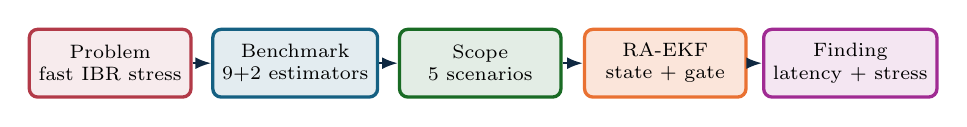
\begin{tikzpicture}[
  every node/.style={font=\scriptsize},
  claim/.style={draw, rounded corners=3pt, very thick, align=center, minimum width=2.05cm, minimum height=0.86cm},
  arr/.style={-{Latex[length=2mm]}, thick, color=ofbInk}
]
\node[claim, fill=ofbRed!10, draw=ofbRed] (p) at (0,0.85) {Problem\\fast IBR stress};
\node[claim, fill=ofbBlue!12, draw=ofbBlue] (b) at (2.35,0.85) {Benchmark\\9+2 estimators};
\node[claim, fill=ofbGreen!12, draw=ofbGreen] (s) at (4.70,0.85) {Scope\\5 scenarios};
\node[claim, fill=ofbGold!18, draw=ofbGold] (m) at (7.05,0.85) {RA-EKF\\state + gate};
\node[claim, fill=ofbViolet!12, draw=ofbViolet] (r) at (9.40,0.85) {Finding\\latency + stress};
\draw[arr] (p) -- (b);
\draw[arr] (b) -- (s);
\draw[arr] (s) -- (m);
\draw[arr] (m) -- (r);
\end{tikzpicture}
\end{center}
\vspace{0.25em}
\begin{columns}[T,onlytextwidth]
\column{0.48\linewidth}
\begin{block}{Stress model}
\small
\begin{itemize}
  \item IBR events can combine ramps, phase jumps, harmonics, and ringdown inside one local relay record.
  \item Scenarios A--C follow IEC/IEEE test philosophy; Scenarios D--E add IBR composite stress.
  \item Estimators are tuned and evaluated using RMSE, peak error, trip-risk duration, settling, and CPU cost.
\end{itemize}
\end{block}
\column{0.47\linewidth}
\begin{block}{Estimator behavior}
\small
\begin{itemize}
  \item RA-EKF reduces false-trip exposure under composite islanding while remaining CPU-feasible.
  \item Windowed methods are accurate in steady state but carry structural observation delay.
  \item Compliance tests alone miss phase-discontinuity and multi-event IBR failure modes.
\end{itemize}
\end{block}
\end{columns}
\end{frame}
\fi

\begin{frame}{Technical contributions}
\begin{columns}[T,onlytextwidth]
\column{0.50\linewidth}
\begin{block}{Scope}
\small
\begin{itemize}
  \item PMU time-stamp certification;
  \item a single universal leaderboard;
  \item hardware latency measurements.
\end{itemize}
\end{block}
\column{0.45\linewidth}
\begin{block}{Contributions}
\small
\begin{itemize}
  \item OpenFreqBench: a reproducible stress-test benchmark and platform for relay-class frequency estimators;
  \item a metric-complete comparison protocol: RMSE, peak error, RoCoF error, $T_{\mathrm{trip}}$, settling, and CPU;
  \item evidence that standard compliance tests miss IBR failure modes;
  \item an adapted RA-EKF, included as one tested estimator with explicit $\dot\omega$ state and event gating.
\end{itemize}
\end{block}
\end{columns}
\vspace{0.35em}
\callout{The benchmark explains why estimator rankings change across objectives, regimes, and compute budgets.}
\end{frame}

\ifbackupframes
\begin{frame}{Scenario waveforms}
\centering
\vspace{-0.25em}
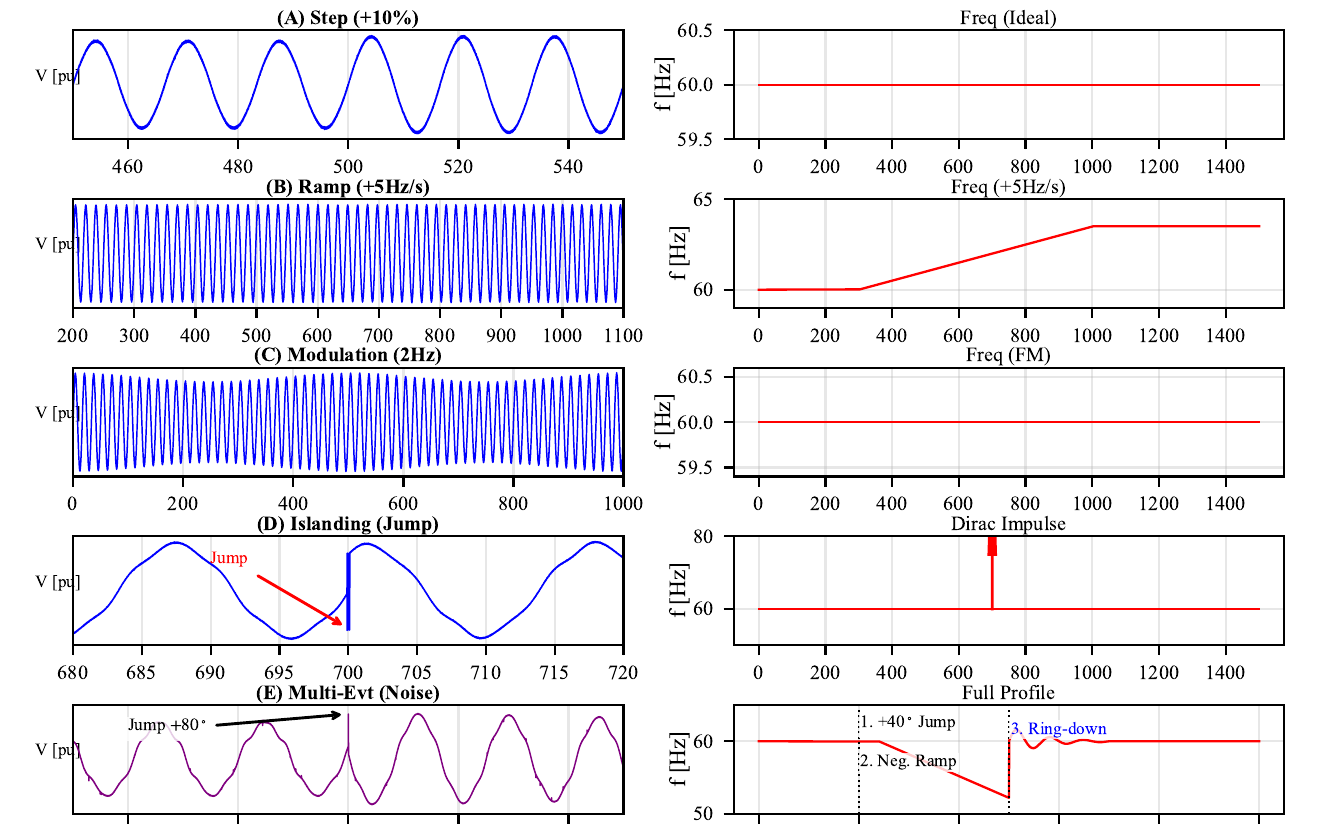
\includegraphics[width=0.98\paperwidth,height=0.78\textheight,keepaspectratio]{figures/doc1_fig1_scenarios.png}
\end{frame}

\begin{frame}{Scenario signatures}
\scriptsize
\renewcommand{\arraystretch}{1.18}
\begin{tabular}{>{\bfseries\raggedright\arraybackslash}p{0.16\linewidth}>{\raggedright\arraybackslash}p{0.30\linewidth}>{\raggedright\arraybackslash}p{0.43\linewidth}}
\toprule
Scenario & Signal & Measurement question \\
\midrule
Scenario A & 10\% voltage magnitude step. & Does amplitude change contaminate frequency tracking? \\
Scenario B & Sustained $+5$ Hz/s frequency ramp. & Can the estimator track RoCoF without excessive lag? \\
Scenario C & 10\% AM modulation at 2 Hz. & Does the estimator preserve steady-state accuracy under modulation? \\
Scenario D & Composite islanding with $+60^\circ$ phase jump, harmonics, interharmonic, and elevated noise. & Does the method recover phase lock without false-trip exposure? \\
Scenario E & Five-second IBR multi-event sequence with harmonics, jumps, negative ramp, ringdown, and impulsive noise. & Response under stacked stress inside one decision window. \\
\bottomrule
\end{tabular}
\vspace{0.35em}
\callout{The scenario suite pairs three standard-style references with two IBR-specific composite stress tests.}
\end{frame}
\fi

\begin{frame}{Estimator selection logic}
\centering
\vspace{-0.2em}
\resizebox{0.98\linewidth}{!}{%
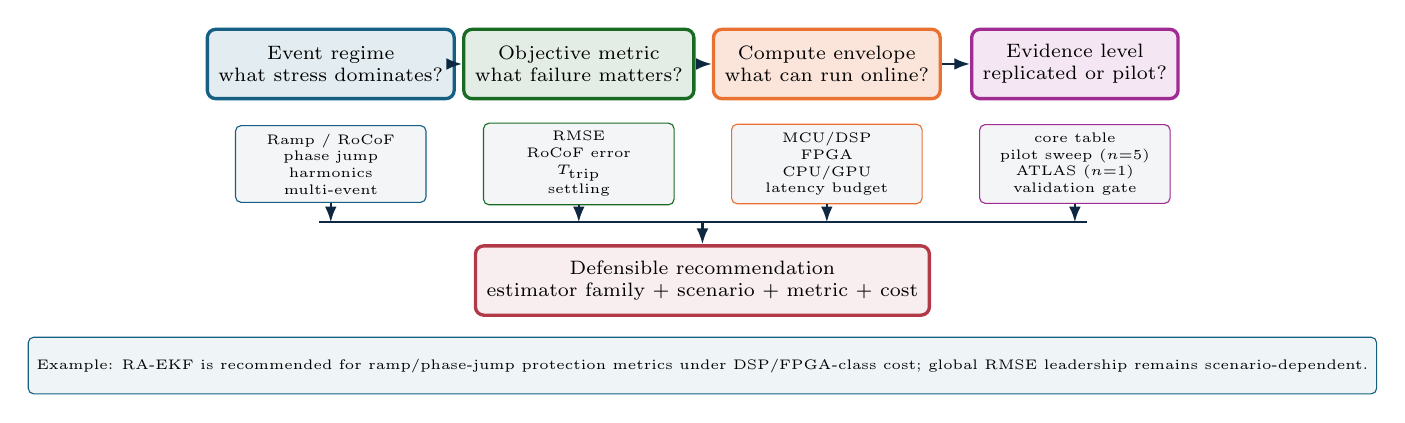
\begin{tikzpicture}[
  every node/.style={font=\scriptsize},
  test/.style={draw, rounded corners=3pt, very thick, align=center, minimum width=2.55cm, minimum height=0.88cm, inner sep=4pt},
  result/.style={draw, rounded corners=2pt, align=center, minimum width=2.42cm, minimum height=0.72cm, inner sep=3pt, font=\tiny},
  arr/.style={-{Latex[length=2mm]}, thick, color=ofbInk}
]
\node[test, fill=ofbBlue!12, draw=ofbBlue] (event) at (0,1.55) {Event regime\\what stress dominates?};
\node[test, fill=ofbGreen!12, draw=ofbGreen] (metric) at (3.15,1.55) {Objective metric\\what failure matters?};
\node[test, fill=ofbGold!18, draw=ofbGold] (cost) at (6.30,1.55) {Compute envelope\\what can run online?};
\node[test, fill=ofbViolet!12, draw=ofbViolet] (evidence) at (9.45,1.55) {Evidence level\\replicated or pilot?};
\node[result, fill=ofbSoft, draw=ofbBlue] (eventr) at (0,0.28) {Ramp / RoCoF\\phase jump\\harmonics\\multi-event};
\node[result, fill=ofbSoft, draw=ofbGreen] (metricr) at (3.15,0.28) {RMSE\\RoCoF error\\$T_{\mathrm{trip}}$\\settling};
\node[result, fill=ofbSoft, draw=ofbGold] (costr) at (6.30,0.28) {MCU/DSP\\FPGA\\CPU/GPU\\latency budget};
\node[result, fill=ofbSoft, draw=ofbViolet] (evidencer) at (9.45,0.28) {core table\\pilot sweep ($n{=}5$)\\ATLAS ($n{=}1$)\\validation gate};
\draw[arr] (event) -- (metric);
\draw[arr] (metric) -- (cost);
\draw[arr] (cost) -- (evidence);
\node[test, fill=ofbRed!9, draw=ofbRed, minimum width=4.2cm] (decision) at (4.72,-1.20) {Defensible recommendation\\estimator family + scenario + metric + cost};
\draw[thick, color=ofbInk] (-0.15,-0.46) -- (9.60,-0.46);
\draw[arr] (eventr.south) -- (0,-0.46);
\draw[arr] (metricr.south) -- (3.15,-0.46);
\draw[arr] (costr.south) -- (6.30,-0.46);
\draw[arr] (evidencer.south) -- (9.45,-0.46);
\draw[arr] (4.72,-0.46) -- (decision.north);
\node[result, fill=ofbBlue!7, draw=ofbBlue, minimum width=10.2cm] at (4.72,-2.28)
{Example: RA-EKF is recommended for ramp/phase-jump protection metrics under DSP/FPGA-class cost; global RMSE leadership remains scenario-dependent.};
\end{tikzpicture}%
}
\end{frame}

\ifbackupframes
\begin{frame}{Evidence layers: benchmark + ATLAS}
\begin{center}
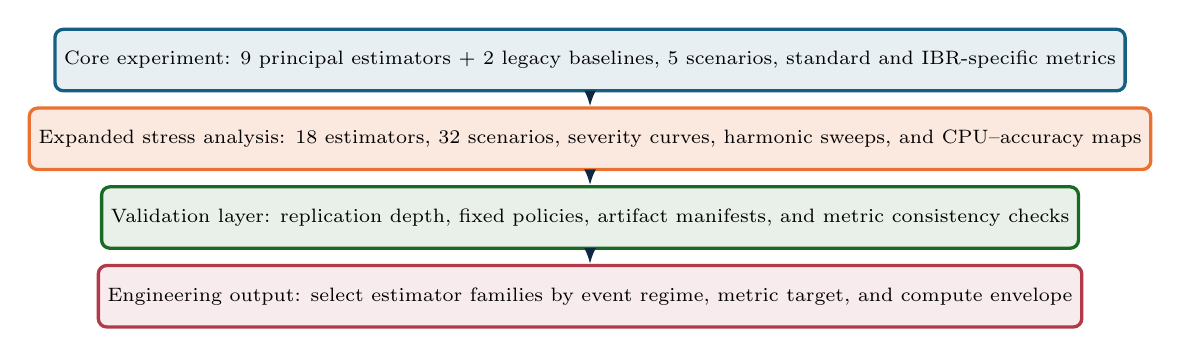
\begin{tikzpicture}[
  every node/.style={font=\scriptsize},
  layer/.style={draw, rounded corners=3pt, very thick, align=center, minimum width=9.6cm, minimum height=0.78cm},
  arr/.style={-{Latex[length=2mm]}, thick, color=ofbInk}
]
\node[layer, fill=ofbBlue!10, draw=ofbBlue] (paper) at (0,1.25) {Core experiment: 9 principal estimators + 2 legacy baselines, 5 scenarios, standard and IBR-specific metrics};
\node[layer, fill=ofbGold!16, draw=ofbGold] (atlas) at (0,0.25) {Expanded stress analysis: 18 estimators, 32 scenarios, severity curves, harmonic sweeps, and CPU--accuracy maps};
\node[layer, fill=ofbGreen!10, draw=ofbGreen] (gate) at (0,-0.75) {Validation layer: replication depth, fixed policies, artifact manifests, and metric consistency checks};
\node[layer, fill=ofbRed!10, draw=ofbRed] (message) at (0,-1.75) {Engineering output: select estimator families by event regime, metric target, and compute envelope};
\draw[arr] (paper) -- (atlas);
\draw[arr] (atlas) -- (gate);
\draw[arr] (gate) -- (message);
\end{tikzpicture}
\end{center}
\vspace{0.2em}
\callout{Controlled cases support the main claims; wider sweeps expose severity trends and replication gaps.}
\end{frame}
\fi

\ifbackupframes
\begin{frame}{From field forensics to estimator tests}
\begin{columns}[T,onlytextwidth]
\column{0.49\linewidth}
\begin{center}
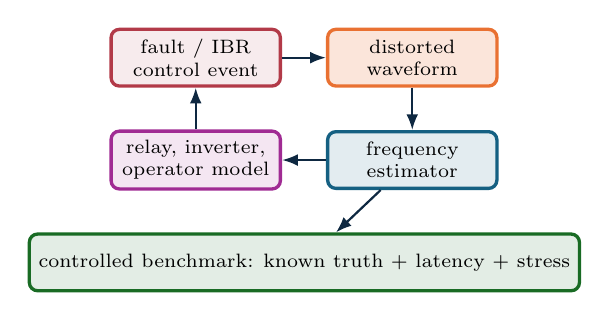
\begin{tikzpicture}[
  every node/.style={font=\scriptsize},
  box/.style={draw, rounded corners=3pt, very thick, align=center, minimum width=2.15cm, minimum height=0.72cm},
  arr/.style={-{Latex[length=2mm]}, thick, color=ofbInk}
]
\node[box, fill=ofbRed!10, draw=ofbRed] (fault) at (0,1.75) {fault / IBR\\control event};
\node[box, fill=ofbGold!18, draw=ofbGold] (wave) at (2.75,1.75) {distorted\\waveform};
\node[box, fill=ofbBlue!12, draw=ofbBlue] (est) at (2.75,0.45) {frequency\\estimator};
\node[box, fill=ofbViolet!12, draw=ofbViolet] (decision) at (0,0.45) {relay, inverter,\\operator model};
\node[box, fill=ofbGreen!12, draw=ofbGreen, minimum width=4.9cm] (bench) at (1.38,-0.85) {controlled benchmark: known truth + latency + stress};
\draw[arr] (fault) -- (wave);
\draw[arr] (wave) -- (est);
\draw[arr] (est) -- (decision);
\draw[arr] (decision) -- (fault);
\draw[arr] (est) -- (bench);
\end{tikzpicture}
\end{center}
\column{0.47\linewidth}
\small
\[
\widehat f_i[k]=\mathcal{E}_i(v[k-L_i:k];\theta_i)
\]
\[
\mathbf{J}_i =
\left[
\mathrm{RMSE}_f,\,
\mathrm{RMSE}_{\dot f},\,
t_s,\,
\tau,\,
C_{\mathrm{CPU}},\,
p_{\mathrm{invalid}}
\right]
\]
\vspace{-0.2em}
\begin{itemize}
  \item A deployable estimator must stay stable during the event, recover quickly, and expose invalid outputs.
  \item It must remain useful when the waveform violates its assumptions.
\end{itemize}
\end{columns}
\end{frame}
\fi

\begin{frame}{IBR disturbances expose the gap}
\scriptsize
\renewcommand{\arraystretch}{1.15}
\setlength{\tabcolsep}{3pt}
\begin{tabular}{>{\raggedright\arraybackslash}p{0.18\linewidth}>{\raggedright\arraybackslash}p{0.22\linewidth}>{\raggedright\arraybackslash}p{0.27\linewidth}>{\raggedright\arraybackslash}p{0.23\linewidth}}
\toprule
\textbf{Event} & \textbf{Observed behavior} & \textbf{Monitoring limitation} & \textbf{Benchmark implication} \\
\midrule
Blue Cut Fire, CA 2016 & Transmission faults caused nearly 1,200 MW of solar PV output loss; NERC linked part of the behavior to near-instantaneous frequency or voltage response. & The critical interval was a distorted, fault-clearing transient on a subsecond timescale. & Test whether estimators confuse waveform distortion with real frequency collapse. \\
Canyon 2 Fire, CA 2017 & Two cleared faults produced 682 MW and 937 MW solar PV reductions. & NERC noted 4 s SCADA could not distinguish momentary cessation from tripping in some cases. & Report latency, settling, invalid samples, event-window behavior, and aggregate error. \\
Odessa events, TX 2021--2022 & More than 1 GW-scale solar reductions followed normally cleared faults far from affected plants. & NERC found controls, protection, and model-fidelity gaps, including effects not captured well by positive-sequence models. & Stress tests must include control-like discontinuities, phase jumps, and model-mismatch regimes. \\
California BESS, 2022 & Normally cleared faults caused abnormal BESS active-power reductions and inverter trips. & Causes included ac overcurrent/overvoltage, dc bus issues, unbalanced currents, and data-quality limits. & Evaluate frequency estimators under unbalance and non-sinusoidal contamination. \\
\bottomrule
\end{tabular}
\vspace{0.35em}
\artifact{NERC disturbance reports; NERC IBR disturbance monitoring white paper}
\end{frame}

\begin{frame}{Standard PMU stream limits}
\begin{columns}[T,onlytextwidth]
\column{0.52\linewidth}
\begin{block}{Fast fault and ride-through}
\scriptsize
IBR controls can react within cycles. A low-rate or heavily filtered frequency estimate may miss the subcycle cause while still showing the delayed consequence.
\end{block}
\begin{block}{Oscillation near reporting-rate limits}
\scriptsize
The Kaua'i 2021 event exhibited 18--20 Hz oscillations after a generator trip. A 30 frame/s phasor stream has a 15 Hz Nyquist limit for phasor-time variations, so oscillations near this range can alias or appear as beating.
\end{block}
\column{0.43\linewidth}
\begin{center}
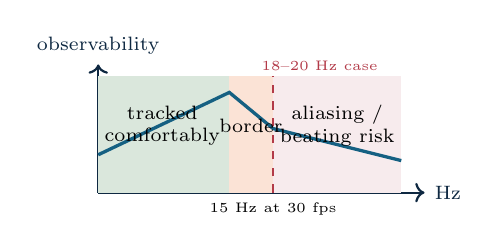
\begin{tikzpicture}[x=0.74cm,y=0.74cm]
  \draw[->, thick, ofbInk] (0,0) -- (5.6,0) node[right,font=\scriptsize] {Hz};
  \draw[->, thick, ofbInk] (0,0) -- (0,2.2) node[above,font=\scriptsize] {observability};
  \fill[ofbGreen!16] (0,0) rectangle (2.25,2.0);
  \fill[ofbGold!20] (2.25,0) rectangle (3.0,2.0);
  \fill[ofbRed!10] (3.0,0) rectangle (5.2,2.0);
  \draw[very thick, ofbBlue] (0,0.65) -- (2.25,1.72) -- (3.0,1.10) -- (5.2,0.55);
  \draw[dashed, thick, ofbRed] (3.0,0) -- (3.0,2.0);
  \node[font=\scriptsize, align=center] at (1.1,1.15) {tracked\\comfortably};
  \node[font=\scriptsize, align=center] at (2.62,1.15) {border};
  \node[font=\scriptsize, align=center] at (4.1,1.15) {aliasing /\\beating risk};
  \node[font=\tiny] at (3.0,-0.28) {15 Hz at 30 fps};
  \node[font=\tiny, ofbRed] at (3.8,2.18) {18--20 Hz case};
\end{tikzpicture}
\end{center}
\vspace{-0.2em}
\begin{block}{Harmonics and interharmonics}
\scriptsize
Standard synchrophasor outputs summarize the fundamental component; harmonic and interharmonic contamination can still dominate estimator failure modes.
\end{block}
\end{columns}
\artifact{Kaua'i 18--20 Hz IBR oscillation analysis; NERC IBR monitoring white paper; IEC/IEEE 60255-118-1}
\end{frame}

\ifbackupframes
\begin{frame}{Benchmark requirements from field cases}
\begin{columns}[T,onlytextwidth]
\column{0.48\linewidth}
\begin{block}{Field-forensic need}
\small
\begin{itemize}
  \item point-on-wave records above 960 samples/s for triggered fault captures;
  \item continuous phasor/dynamic disturbance records at $\geq 30$ samples/s;
  \item inverter fault codes, mode changes, and control states;
  \item traceable event replay for model validation.
\end{itemize}
\end{block}
\column{0.47\linewidth}
\begin{block}{Benchmark analogue}
\small
\begin{itemize}
  \item known-truth synthetic scenarios with steps, ramps, phase jumps, THD, and interharmonics;
  \item estimator outputs logged as time series and scalar summaries;
  \item latency, CPU, invalid outputs, and settling treated as first-class metrics;
  \item CSV/JSON artifacts regenerated into figures and tables.
\end{itemize}
\end{block}
\end{columns}
\vspace{0.25em}
\callout{Field oscillography gives realism; controlled synthetic truth isolates which estimator family fails first.}
\end{frame}

\begin{frame}{Graphical abstract}
\begin{center}
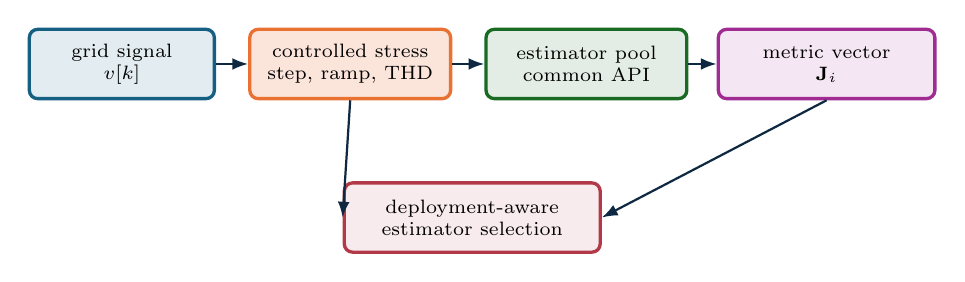
\begin{tikzpicture}[
  every node/.style={font=\scriptsize},
  box/.style={draw, rounded corners=3pt, align=center, very thick, minimum height=0.88cm},
  arr/.style={-{Latex[length=2mm]}, thick, color=ofbInk}
]
\node[box, fill=ofbBlue!12, draw=ofbBlue, minimum width=2.35cm] (grid) at (0,0.8) {grid signal\\$v[k]$};
\node[box, fill=ofbGold!18, draw=ofbGold, minimum width=2.55cm] (stress) at (2.9,0.8) {controlled stress\\step, ramp, THD};
\node[box, fill=ofbGreen!12, draw=ofbGreen, minimum width=2.55cm] (est) at (5.9,0.8) {estimator pool\\common API};
\node[box, fill=ofbViolet!12, draw=ofbViolet, minimum width=2.75cm] (metric) at (8.95,0.8) {metric vector\\$\mathbf{J}_i$};
\node[box, fill=ofbRed!10, draw=ofbRed, minimum width=3.25cm] (select) at (4.45,-1.15) {deployment-aware\\estimator selection};
\draw[arr] (grid) -- (stress);
\draw[arr] (stress) -- (est);
\draw[arr] (est) -- (metric);
\draw[arr] (metric.south) -- (select.east);
\draw[arr] (stress.south) -- (select.west);
\end{tikzpicture}
\end{center}
\vspace{0.3em}
\begin{columns}[T,onlytextwidth]
\column{0.32\linewidth}
\tagpill{ofbBlue}{Accuracy}\\
\scriptsize Frequency RMSE and settling.
\column{0.32\linewidth}
\tagpill{ofbViolet}{Dynamics}\\
\scriptsize RoCoF tracking and sensitivity.
\column{0.32\linewidth}
\tagpill{ofbGold}{Deployability}\\
\scriptsize CPU, latency, and jitter.
\end{columns}
\end{frame}

\begin{frame}{Study logic}
\begin{center}
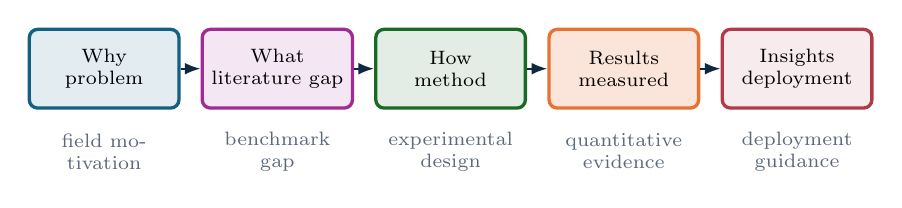
\begin{tikzpicture}[
  every node/.style={font=\scriptsize},
  stage/.style={draw, rounded corners=3pt, very thick, align=center, minimum width=2.25cm, minimum height=1.0cm},
  arr/.style={-{Latex[length=2mm]}, thick, color=ofbInk}
]
\node[stage, fill=ofbBlue!12, draw=ofbBlue, minimum width=1.9cm] (p) at (0,0) {Why\\problem};
\node[stage, fill=ofbViolet!12, draw=ofbViolet, minimum width=1.9cm] (l) at (2.2,0) {What\\literature gap};
\node[stage, fill=ofbGreen!12, draw=ofbGreen, minimum width=1.9cm] (m) at (4.4,0) {How\\method};
\node[stage, fill=ofbGold!18, draw=ofbGold, minimum width=1.9cm] (r) at (6.6,0) {Results\\measured};
\node[stage, fill=ofbRed!10, draw=ofbRed, minimum width=1.9cm] (d) at (8.8,0) {Insights\\deployment};
\draw[arr] (p) -- (l);
\draw[arr] (l) -- (m);
\draw[arr] (m) -- (r);
\draw[arr] (r) -- (d);
\node[align=center, text=ofbMuted, text width=1.7cm] at (0,-1.05) {field motivation};
\node[align=center, text=ofbMuted, text width=1.7cm] at (2.2,-1.05) {benchmark gap};
\node[align=center, text=ofbMuted, text width=1.7cm] at (4.4,-1.05) {experimental design};
\node[align=center, text=ofbMuted, text width=1.7cm] at (6.6,-1.05) {quantitative evidence};
\node[align=center, text=ofbMuted, text width=1.7cm] at (8.8,-1.05) {deployment guidance};
\end{tikzpicture}
\end{center}
\vspace{0.35em}
\callout{The argument moves from grid events to estimator qualification: define the stress, run matched estimators, evaluate multiple metrics, and map the result to deployment regimes.}
\end{frame}
\fi


\begin{frame}{Research problem}
\begin{columns}[T,onlytextwidth]
\column{0.55\linewidth}
\begin{itemize}
  \item Low-inertia IBR grids require reliable local frequency estimates during ramps, phase jumps, harmonic distortion, ringdown, and mixed dynamic events.
  \item Classical estimators often trade off responsiveness, noise rejection, latency, and computational load.
  \item Modern model-based and data-driven estimators improve some regimes, but can be difficult to compare fairly.
  \item Existing comparisons often under-specify seeds, disturbance families, tuning policy, trip-risk, structural latency, or computational cost.
\end{itemize}
\column{0.40\linewidth}
\begin{block}{Research gap}
The literature needs a reproducible benchmark that connects estimator error to protection-oriented risk, settling behavior, and deployability.
\end{block}
\end{columns}
\end{frame}

\ifbackupframes
\begin{frame}{Research questions}
\begin{enumerate}
  \item Which estimator families lead each disturbance family: ramps, magnitude steps, modulation, phase jumps, OOB interference, harmonics, ringdown, and composite IBR events?
  \item When do RMSE, peak error, trip-risk duration, and settling time select different estimators?
  \item How does CPU cost change a ranking that appears favorable under accuracy alone?
  \item Which scenarios are hardest, and what do they reveal about IBR-oriented protection measurement?
  \item How do severity sweeps change the interpretation of the five-scenario benchmark?
\end{enumerate}
\vspace{0.4em}
\callout{The central result is conditional selection: there is no universal estimator; the defensible choice depends on disturbance family, objective metric, and compute budget.}
\end{frame}
\fi


\begin{frame}{Benchmark gap in prior work}
\scriptsize
The field is mature in standards, metrology, open platforms, real datasets, and single-method studies. The missing layer is a reproducible, estimator-level benchmark that compares many algorithms under identical synthetic truth and deployment metrics.
\vspace{0.30em}
\renewcommand{\arraystretch}{1.18}
\begin{tabular}{>{\raggedright\arraybackslash}p{0.21\linewidth}>{\raggedright\arraybackslash}p{0.31\linewidth}>{\raggedright\arraybackslash}p{0.37\linewidth}}
\toprule
\textbf{Prior benchmark type} & \textbf{Strength} & \textbf{Gap for estimator-family comparison} \\
\midrule
IEC/IEEE PMU compliance & Defines synchrophasor, frequency, RoCoF, static/dynamic compliance tests & Leaves algorithm choice, family comparison, and CPU/latency outside the estimator report. \\
NIST PMU assessment/calibration & Provides metrological evaluation of PMU devices against standard requirements & Focuses on instruments and compliance behavior rather than a large matrix of open estimator implementations under controlled tuning policy. \\
OpenPMU / openPDC ecosystem & Enables open PMU construction and synchrophasor stream processing & Infrastructure-oriented, with no controlled estimator matrix using matched seeds and stress sweeps. \\
Open real PMU datasets & Supply realistic events for detection and application development & Truth is partially latent; hard to isolate causal stress factors or compute estimator error against known $f_{\mathrm{true}}[k]$. \\
Single-study algorithm comparisons & Give detailed evidence for selected methods or scenarios & Usually limited estimator sets, limited artifact contract, and incomplete deployability metrics. \\
\bottomrule
\end{tabular}
\vspace{0.4em}
\callout{Compliance tests define requirements, operational data define realism, and controlled synthetic truth isolates estimator behavior under reproducible stress.}
\artifact{IEC/IEEE 60255-118-1:2018; NISTIR 8106; OpenPMU; openPDC; FNET/GridEye; LBNL Open micro-PMU; PNNL open PMU event library}
\end{frame}

\ifbackupframes
\begin{frame}{Benchmark contribution}
\begin{center}
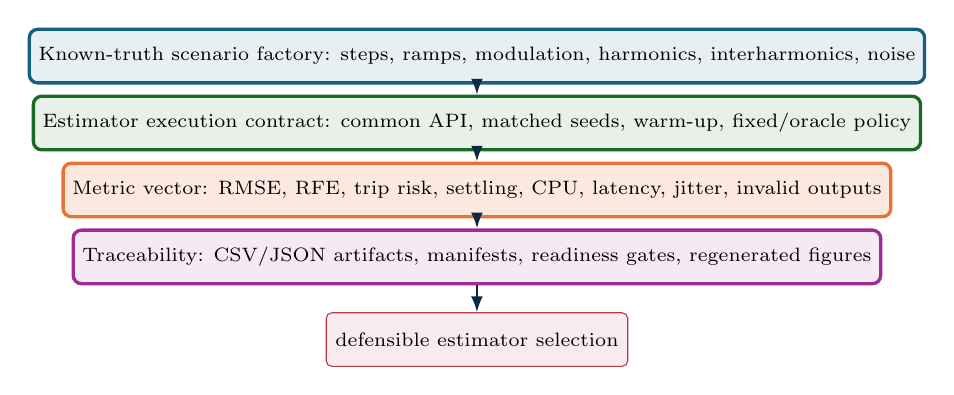
\begin{tikzpicture}[
  every node/.style={font=\scriptsize},
  layer/.style={draw, rounded corners=3pt, very thick, align=center, minimum width=8.4cm, minimum height=0.68cm},
  side/.style={draw, rounded corners=2pt, align=center, minimum width=2.6cm, minimum height=0.68cm},
  arr/.style={-{Latex[length=2mm]}, thick, color=ofbInk}
]
\node[layer, fill=ofbBlue!10, draw=ofbBlue] (l1) at (0,1.55) {Known-truth scenario factory: steps, ramps, modulation, harmonics, interharmonics, noise};
\node[layer, fill=ofbGreen!10, draw=ofbGreen] (l2) at (0,0.70) {Estimator execution contract: common API, matched seeds, warm-up, fixed/oracle policy};
\node[layer, fill=ofbGold!16, draw=ofbGold] (l3) at (0,-0.15) {Metric vector: RMSE, RFE, trip risk, settling, CPU, latency, jitter, invalid outputs};
\node[layer, fill=ofbViolet!10, draw=ofbViolet] (l4) at (0,-1.00) {Traceability: CSV/JSON artifacts, manifests, readiness gates, regenerated figures};
\node[side, fill=ofbRed!10, draw=ofbRed] (goal) at (0,-2.05) {defensible estimator selection};
\draw[arr] (l1) -- (l2);
\draw[arr] (l2) -- (l3);
\draw[arr] (l3) -- (l4);
\draw[arr] (l4) -- (goal);
\end{tikzpicture}
\end{center}
\vspace{0.15em}
\callout{The experimental system explains why estimator rankings change across objectives and regimes.}
\end{frame}
\fi

\begin{frame}{Benchmark comparison axes}
\scriptsize
\setlength{\tabcolsep}{4.5pt}
\renewcommand{\arraystretch}{1.16}
\begin{center}
\resizebox{0.98\linewidth}{!}{%
\begin{tabular}{>{\bfseries\raggedright\arraybackslash}p{0.22\linewidth}ccccc}
\toprule
Evidence source & Known truth & IBR composite stress & Trip-risk & CPU/latency & Reproducible artifacts \\
\midrule
IEC/IEEE-style compliance & \cellcolor{ofbGreen!22}Yes & \cellcolor{ofbRed!18}Limited & \cellcolor{ofbRed!18}No & \cellcolor{ofbRed!18}No & \cellcolor{ofbGold!22}Device-dependent \\
Field PMU/DFR data & \cellcolor{ofbRed!18}No & \cellcolor{ofbGreen!22}Yes & \cellcolor{ofbGold!22}Possible & \cellcolor{ofbRed!18}No & \cellcolor{ofbGold!22}Dataset-dependent \\
Single-method studies & \cellcolor{ofbGreen!22}Often & \cellcolor{ofbGold!22}Partial & \cellcolor{ofbGold!22}Partial & \cellcolor{ofbGold!22}Partial & \cellcolor{ofbRed!18}Often limited \\
Estimator benchmark & \cellcolor{ofbGreen!22}Yes & \cellcolor{ofbGreen!22}Yes & \cellcolor{ofbGreen!22}Yes & \cellcolor{ofbGreen!22}Yes & \cellcolor{ofbGreen!22}Yes \\
\bottomrule
\end{tabular}%
}
\end{center}
\vspace{0.35em}
\begin{columns}[T,onlytextwidth]
\column{0.48\linewidth}
\begin{block}{Measured outputs}
\small
The same voltage trace is scored by RMSE, peak error, RoCoF error, trip exposure, settling, CPU, and structural latency.
\end{block}
\column{0.47\linewidth}
\begin{block}{Interpretive effect}
\small
An estimator can pass standard cases and still fail a composite IBR event; it can also be accurate but too delayed or costly for protection-adjacent use.
\end{block}
\end{columns}
\end{frame}

\begin{frame}{OpenFreqBench platform}
\vspace{-0.25em}
\begin{center}
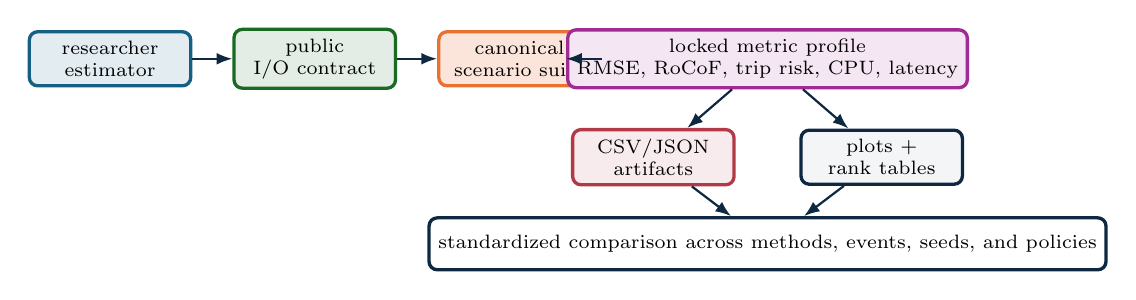
\begin{tikzpicture}[
  every node/.style={font=\scriptsize},
  box/.style={draw, rounded corners=3pt, very thick, align=center, minimum width=2.05cm, minimum height=0.66cm},
  wide/.style={draw, rounded corners=3pt, very thick, align=center, minimum width=4.55cm, minimum height=0.66cm},
  arr/.style={-{Latex[length=2mm]}, thick, color=ofbInk}
]
\node[box, fill=ofbBlue!12, draw=ofbBlue] (method) at (0,1.10) {researcher\\estimator};
\node[box, fill=ofbGreen!12, draw=ofbGreen] (api) at (2.60,1.10) {public\\I/O contract};
\node[box, fill=ofbGold!18, draw=ofbGold] (scen) at (5.20,1.10) {canonical\\scenario suite};
\node[wide, fill=ofbViolet!12, draw=ofbViolet] (metrics) at (8.35,1.10) {locked metric profile\\RMSE, RoCoF, trip risk, CPU, latency};
\node[box, fill=ofbRed!10, draw=ofbRed] (art) at (6.90,-0.15) {CSV/JSON\\artifacts};
\node[box, fill=ofbSoft, draw=ofbInk] (plots) at (9.80,-0.15) {plots +\\rank tables};
\node[wide, fill=white, draw=ofbInk] (compare) at (8.35,-1.25) {standardized comparison across methods, events, seeds, and policies};
\draw[arr] (method) -- (api);
\draw[arr] (api) -- (scen);
\draw[arr] (scen) -- (metrics);
\draw[arr] (metrics) -- (art);
\draw[arr] (metrics) -- (plots);
\draw[arr] (art) -- (compare);
\draw[arr] (plots) -- (compare);
\end{tikzpicture}
\end{center}
\vspace{-0.25em}
\begin{columns}[T,onlytextwidth]
\column{0.31\linewidth}
\begin{block}{Researchers add}
\scriptsize
Estimator code, parameters, and hypotheses through the public contract.
\end{block}
\column{0.33\linewidth}
\begin{block}{Platform fixes}
\scriptsize
Truth signals, sampling, seeds, tuning policy, metric formulas, and schema.
\end{block}
\column{0.31\linewidth}
\begin{block}{Outputs}
\scriptsize
Benchmark reports, metric tables, plots, manifests, and readiness gates.
\end{block}
\end{columns}
\vspace{0.15em}
\callout{OpenFreqBench turns a new estimator into a repeatable benchmark entry instead of a one-off comparison.}
\end{frame}


\begin{frame}{Experimental method}
\begin{columns}[T,onlytextwidth]
\column{0.55\linewidth}
\begin{center}
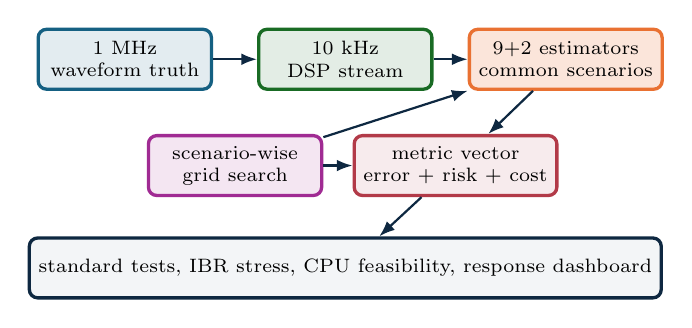
\begin{tikzpicture}[
  every node/.style={font=\scriptsize},
  box/.style={draw, rounded corners=3pt, very thick, align=center, minimum width=2.2cm, minimum height=0.76cm},
  arr/.style={-{Latex[length=2mm]}, thick, color=ofbInk}
]
\node[box, fill=ofbBlue!12, draw=ofbBlue] (wave) at (0,1.2) {1 MHz\\waveform truth};
\node[box, fill=ofbGreen!12, draw=ofbGreen] (dec) at (2.8,1.2) {10 kHz\\DSP stream};
\node[box, fill=ofbGold!18, draw=ofbGold] (est) at (5.6,1.2) {9+2 estimators\\common scenarios};
\node[box, fill=ofbViolet!12, draw=ofbViolet] (tune) at (1.4,-0.15) {scenario-wise\\grid search};
\node[box, fill=ofbRed!10, draw=ofbRed] (met) at (4.2,-0.15) {metric vector\\error + risk + cost};
\node[box, fill=ofbSoft, draw=ofbInk, minimum width=5.8cm] (paper) at (2.8,-1.45) {standard tests, IBR stress, CPU feasibility, response dashboard};
\draw[arr] (wave) -- (dec);
\draw[arr] (dec) -- (est);
\draw[arr] (est) -- (met);
\draw[arr] (tune) -- (est);
\draw[arr] (tune) -- (met);
\draw[arr] (met) -- (paper);
\end{tikzpicture}
\end{center}
\column{0.41\linewidth}
\begin{block}{Measurement setting}
\small
Local, non-time-synchronized relay-class frequency tracking from a decimated 10 kHz stream; PMU timestamp certification is outside scope.
\end{block}
\begin{block}{Experimental principle}
\small
Each estimator--scenario pair is tuned within a declared grid, then compared using RMSE, peak error, trip exposure, settling, and CPU.
\end{block}
\end{columns}
\vspace{0.25em}
\artifact{Methodology and test framework}
\end{frame}

\begin{frame}{RA-EKF mechanism}
\begin{columns}[T,onlytextwidth]
\column{0.50\linewidth}
\begin{block}{State augmentation}
\small
\[
x_k=[\theta_k,\omega_k,A_k,\dot\omega_k]^\top,\qquad \omega=2\pi f
\]
\[
\theta_k=\theta_{k-1}+\omega_{k-1}\Delta t+\frac{1}{2}\dot\omega_{k-1}\Delta t^2
\]
\[
\omega_k=\omega_{k-1}+\dot\omega_{k-1}\Delta t
\]
\end{block}
\column{0.45\linewidth}
\begin{block}{IBR-specific stress response}
\small
\[
Q_k=\mathrm{clip}(r_k,0.25,4)\,Q_{\mathrm{base}},
\qquad
r_k=\frac{|\nu_k|}{\hat\sigma_\nu}
\]
\begin{itemize}
  \item \textbf{Covariance scaling}: inflate process noise under transients, deflate near steady state.
  \item \textbf{Event gating}: when $|\nu_k|>\gamma\hat\sigma_\nu$, softly reset $\theta_k$ while preserving $\omega_k$ and $\dot\omega_k$.
\end{itemize}
\end{block}
\end{columns}
\vspace{0.25em}
\callout{RA-EKF extends the EKF baseline with an explicit RoCoF state and event-aware covariance behavior for phase-jump recovery and steady-state tracking.}
\end{frame}

\begin{frame}{Metrics and decision variables}
\small
\begin{columns}[T,onlytextwidth]
\column{0.48\linewidth}
\begin{block}{Error and recovery}
\[
e[k]=\widehat f[k]-f_{\mathrm{true}}[k]
\]
\[
\mathrm{RMSE}=\sqrt{\frac{1}{N}\sum_k e[k]^2}
\]
\[
E_{\max}=\max_k |e[k]|
\]
\end{block}
\column{0.47\linewidth}
\begin{block}{Protection-oriented risk}
\[
T_{\mathrm{trip}}=\Delta t\sum_k \mathbf{1}\{|e[k]|>0.5\ \mathrm{Hz}\}
\]
\[
t_s=\min\{t:\ |e[\tau]|\leq \epsilon,\ \forall \tau\geq t\}
\]
\[
C_{\mathrm{CPU}}=\mathrm{mean\ time/sample}
\]
\end{block}
\end{columns}
\vspace{0.2em}
\callout{The 0.5 Hz threshold is a protection-oriented risk proxy. The metric set separates average error, transient severity, trip exposure, settling, and compute cost.}
\end{frame}

\ifbackupframes
\begin{frame}{Scenario design: five stress cases}
\scriptsize
\setlength{\tabcolsep}{4pt}
\renewcommand{\arraystretch}{1.12}
\begin{tabular}{>{\bfseries\raggedright\arraybackslash}p{0.12\linewidth}>{\raggedright\arraybackslash}p{0.33\linewidth}>{\raggedright\arraybackslash}p{0.45\linewidth}}
\toprule
\textbf{Case} & \textbf{Disturbance} & \textbf{Purpose} \\
\midrule
A & $+10\%$ voltage magnitude step. & Standard-style amplitude decoupling test. \\
B & $+5$ Hz/s frequency ramp. & RoCoF tracking and lag under sustained acceleration. \\
C & 10\% AM modulation at 2 Hz. & Steady-state modulation and noise sensitivity. \\
D & Composite islanding: $+60^\circ$ phase jump with harmonics/interharmonic and elevated noise. & Phase-jump recovery and false-trip exposure beyond standard tests. \\
E & IBR multi-event: harmonics, $+40^\circ$ jump, $-6$ Hz/s ramp, $+80^\circ$ jump, ringdown, impulsive noise. & Stacked stress resembling local IBR event records. \\
\bottomrule
\end{tabular}
\vspace{0.35em}
\callout{The design deliberately separates standard-style cases (A--C) from IBR-specific composite stress (D--E), which is where compliance pass/fail alone becomes inadequate.}
\artifact{Scenario definitions and Fig. 1}
\end{frame}
\fi

\begin{frame}{Scenario suite}
\begin{columns}[T,onlytextwidth]
\column{0.64\linewidth}
\centering
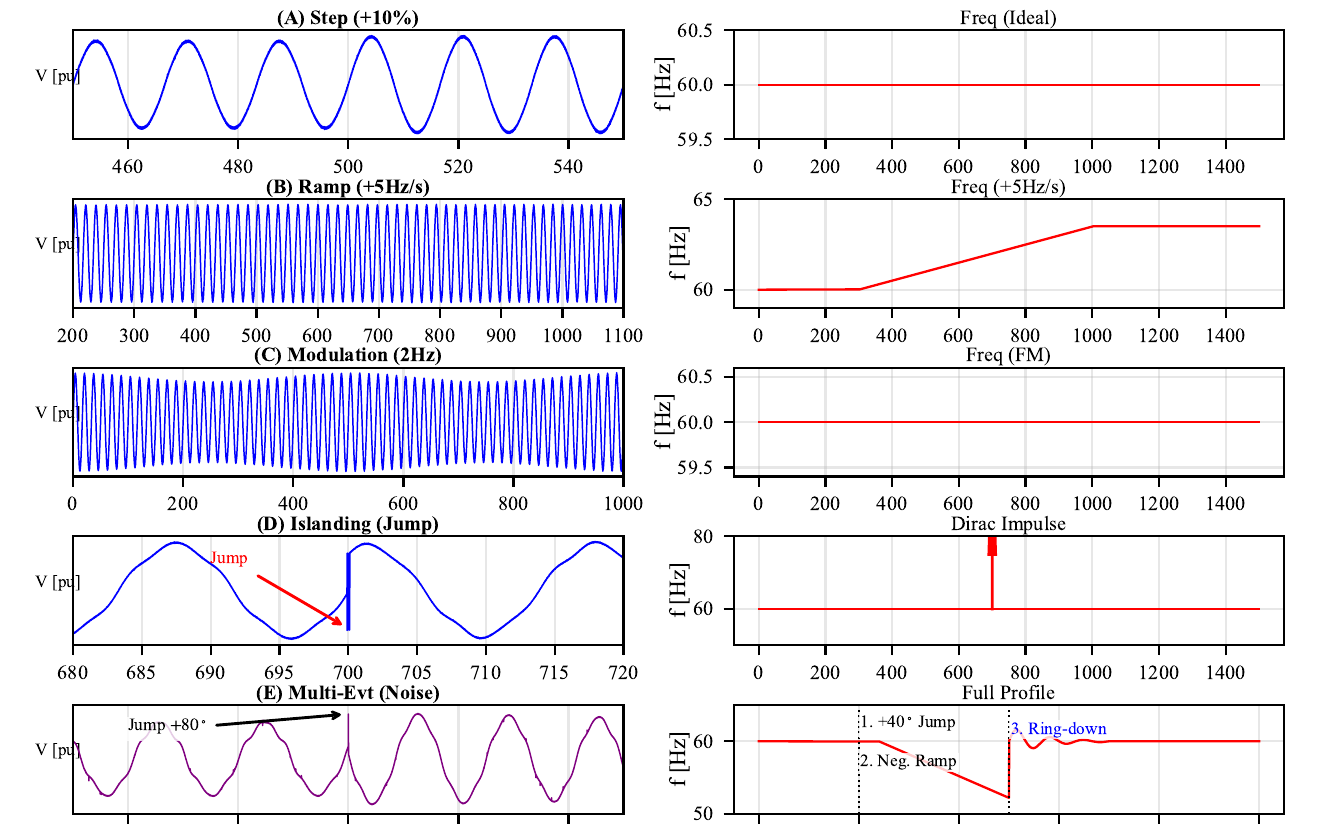
\includegraphics[width=\linewidth]{figures/doc1_fig1_scenarios.png}
\column{0.31\linewidth}
\begin{block}{Scenario structure}
\scriptsize
\begin{itemize}
  \item A--C are standard-style references.
  \item D introduces phase discontinuity and harmonic stress.
  \item E stacks the event mechanisms that standards isolate.
  \item RMSE, $T_{\mathrm{trip}}$, and CPU need a joint reading.
\end{itemize}
\end{block}
\end{columns}
\end{frame}

\begin{frame}{Estimator families}
\begin{columns}[T,onlytextwidth]
\column{0.30\linewidth}
\begin{block}{Loop-based}
\small
SRF-PLL, SOGI-FLL.
\end{block}
\begin{block}{Window-based}
\small
IpDFT, TFT.
\end{block}
\column{0.31\linewidth}
\begin{block}{Model-based / stochastic}
\small
EKF, UKF, RA-EKF.
\end{block}
\begin{block}{Adaptive and data-driven}
\small
VFF-RLS, Koopman (RK-DPMU), PI-GRU.
\end{block}
\column{0.33\linewidth}
\begin{block}{Legacy baselines}
\small
RLS and TKEO are retained as comparison references outside the recommended deployment set.
\end{block}
\begin{block}{Interpretation rule}
\small
These families occupy different latency and stress-sensitivity positions. The comparison tracks where each family wins, degrades, and fails.
\end{block}
\end{columns}
\end{frame}

\ifbackupframes
\begin{frame}{Signal and disturbance model}
\begin{columns}[T,onlytextwidth]
\column{0.52\linewidth}
\begin{block}{Observed single-phase voltage}
\scriptsize
\[
\begin{aligned}
v[k] ={}&
\textcolor{ofbBlue}{A[k]\sin(\theta[k]+\phi_0)}\\
&+ \textcolor{ofbGold}{\sum_{h\in\mathcal{H}} a_h[k]\sin(h\theta[k]+\phi_h)}
+ \textcolor{ofbRed}{\eta[k]}
\end{aligned}
\]
\[
\begin{aligned}
\textcolor{ofbGreen}{f_{\mathrm{true}}[k]} &=
\frac{1}{2\pi}\frac{d\theta(t)}{dt}\bigg|_{t=k/f_s}\\
\textcolor{ofbViolet}{\mathrm{RoCoF}[k]} &=
\frac{df_{\mathrm{true}}(t)}{dt}\bigg|_{t=k/f_s}
\end{aligned}
\]
\end{block}
\column{0.43\linewidth}
\begin{center}
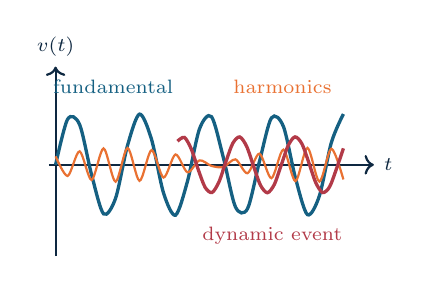
\begin{tikzpicture}[scale=0.86, every node/.style={font=\scriptsize}]
  \draw[->, thick, ofbInk] (-0.1,0) -- (4.7,0) node[right] {$t$};
  \draw[->, thick, ofbInk] (0,-1.35) -- (0,1.45) node[above] {$v(t)$};
  \draw[domain=0:4.25, smooth, variable=\x, ofbBlue, very thick]
    plot ({\x},{sin(360*\x)*0.75});
  \draw[domain=0:4.25, smooth, variable=\x, ofbRust, thick]
    plot ({\x},{0.25*sin(1080*\x+30)});
  \draw[domain=1.8:4.25, smooth, variable=\x, ofbRed, very thick]
    plot ({\x},{0.75*sin(360*(1.2*\x))*0.55});
  \node[ofbBlue, align=left] at (0.85,1.15) {fundamental};
  \node[ofbRust, align=left] at (3.35,1.15) {harmonics};
  \node[ofbRed, align=left] at (3.20,-1.05) {dynamic event};
\end{tikzpicture}
\end{center}
\end{columns}
\vspace{0.25em}
\callout{Known $f_{\mathrm{true}}[k]$ lets each estimator be tested under explicit violations of ideal sinusoidal assumptions.}
\end{frame}

\begin{frame}{Experimental design factors}
\begin{center}
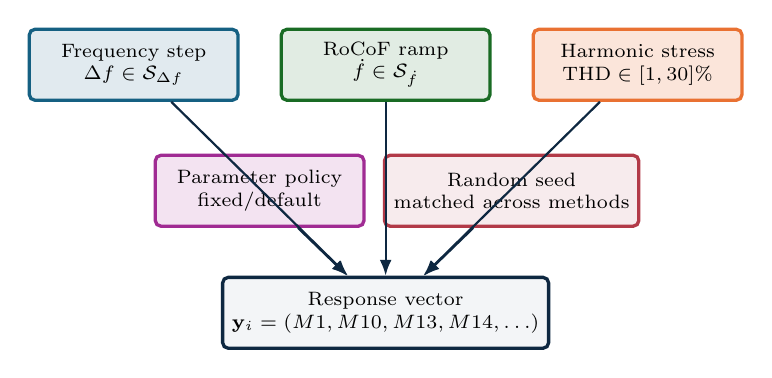
\begin{tikzpicture}[
  every node/.style={font=\scriptsize},
  factor/.style={draw, rounded corners=2pt, align=center, minimum width=2.65cm, minimum height=0.9cm, very thick},
  arr/.style={-{Latex[length=2mm]}, thick, color=ofbInk}
]
\node[factor, fill=ofbBlue!13, draw=ofbBlue] (step) at (0,1.3) {Frequency step\\$\Delta f \in \mathcal{S}_{\Delta f}$};
\node[factor, fill=ofbGreen!13, draw=ofbGreen] (rocof) at (3.2,1.3) {RoCoF ramp\\$\dot f \in \mathcal{S}_{\dot f}$};
\node[factor, fill=ofbGold!18, draw=ofbGold] (harm) at (6.4,1.3) {Harmonic stress\\$\mathrm{THD}\in[1,30]\%$};
\node[factor, fill=ofbViolet!13, draw=ofbViolet] (policy) at (1.6,-0.3) {Parameter policy\\fixed/default};
\node[factor, fill=ofbRed!10, draw=ofbRed] (seed) at (4.8,-0.3) {Random seed\\matched across methods};
\node[factor, fill=ofbSoft, draw=ofbInk] (response) at (3.2,-1.85) {Response vector\\$\mathbf{y}_i=(M1,M10,M13,M14,\ldots)$};
\draw[arr] (step) -- (response);
\draw[arr] (rocof) -- (response);
\draw[arr] (harm) -- (response);
\draw[arr] (policy) -- (response);
\draw[arr] (seed) -- (response);
\end{tikzpicture}
\end{center}
\vspace{0.2em}
\begin{itemize}
  \item The design is factorial in stress type, stress level, estimator family, policy, and Monte Carlo seed.
  \item The response vector keeps accuracy, recovery, latency, and cost as separate outputs.
\end{itemize}
\end{frame}

\begin{frame}{Benchmark methodology}
\begin{center}
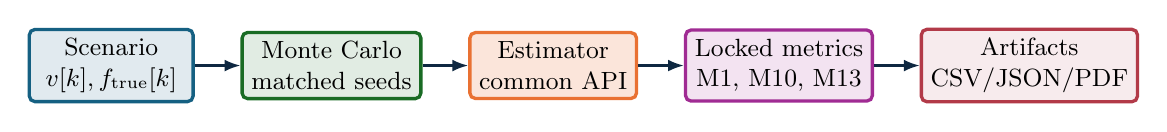
\begin{tikzpicture}[
  node distance=0.58cm,
  box/.style={draw, rounded corners=2pt, align=center, minimum width=2.08cm, minimum height=0.78cm, font=\small, very thick},
  arr/.style={-{Latex[length=2mm]}, thick, color=ofbInk}
]
\node[box, fill=ofbBlue!13, draw=ofbBlue] (scenario) {Scenario\\$v[k], f_{\mathrm{true}}[k]$};
\node[box, fill=ofbGreen!13, draw=ofbGreen, right=of scenario] (mc) {Monte Carlo\\matched seeds};
\node[box, fill=ofbGold!18, draw=ofbGold, right=of mc] (est) {Estimator\\common API};
\node[box, fill=ofbViolet!13, draw=ofbViolet, right=of est] (metrics) {Locked metrics\\M1, M10, M13};
\node[box, fill=ofbRed!10, draw=ofbRed, right=of metrics] (artifacts) {Artifacts\\CSV/JSON/PDF};
\draw[arr] (scenario) -- (mc);
\draw[arr] (mc) -- (est);
\draw[arr] (est) -- (metrics);
\draw[arr] (metrics) -- (artifacts);
\end{tikzpicture}
\end{center}
\vspace{0.35em}
\begin{itemize}
  \item Common sampling profile: $f_s=10$ kHz under \texttt{canonical-single-phase-v1}.
  \item Metrics are defined in code and documentation; scenario configuration is separate from metric definitions.
  \item Every result traces back to reports, manifests, CSV tables, and benchmark metadata.
\end{itemize}
\artifact{docs/METHODS.md}
\end{frame}

\begin{frame}{Estimator execution contract}
\begin{center}
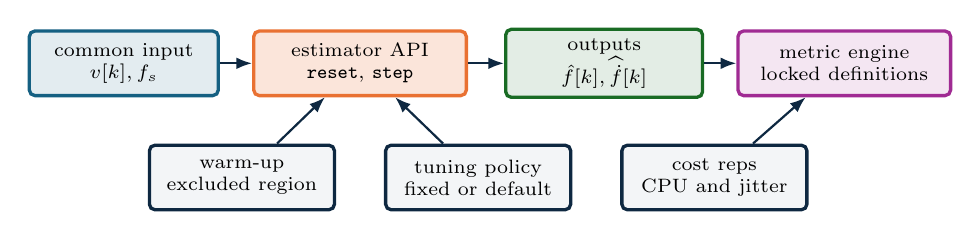
\begin{tikzpicture}[
  every node/.style={font=\scriptsize},
  box/.style={draw, rounded corners=2pt, align=center, minimum height=0.82cm, very thick},
  arr/.style={-{Latex[length=2mm]}, thick, color=ofbInk}
]
\node[box, fill=ofbBlue!12, draw=ofbBlue, minimum width=2.4cm] (input) at (0,0) {common input\\$v[k], f_s$};
\node[box, fill=ofbGold!18, draw=ofbGold, minimum width=2.7cm] (api) at (3.0,0) {estimator API\\\texttt{reset}, \texttt{step}};
\node[box, fill=ofbGreen!12, draw=ofbGreen, minimum width=2.5cm] (output) at (6.1,0) {outputs\\$\hat f[k], \widehat{\dot f}[k]$};
\node[box, fill=ofbViolet!12, draw=ofbViolet, minimum width=2.7cm] (metric) at (9.15,0) {metric engine\\locked definitions};
\draw[arr] (input) -- (api);
\draw[arr] (api) -- (output);
\draw[arr] (output) -- (metric);
\node[box, fill=ofbSoft, draw=ofbInk, minimum width=2.35cm] (warm) at (1.5,-1.45) {warm-up\\excluded region};
\node[box, fill=ofbSoft, draw=ofbInk, minimum width=2.35cm] (tune) at (4.5,-1.45) {tuning policy\\fixed or default};
\node[box, fill=ofbSoft, draw=ofbInk, minimum width=2.35cm] (cost) at (7.5,-1.45) {cost reps\\CPU and jitter};
\draw[arr] (warm) -- (api);
\draw[arr] (tune) -- (api);
\draw[arr] (cost) -- (metric);
\end{tikzpicture}
\end{center}
\vspace{0.2em}
\begin{itemize}
  \item Fairness is enforced through identical input traces, matched random seeds, common warm-up handling, and a uniform output interface.
  \item Computational performance is measured as a response variable for deployability.
\end{itemize}
\end{frame}

\begin{frame}{Metric equations}
\begin{columns}[T,onlytextwidth]
\column{0.48\linewidth}
\begin{block}{Frequency and derivative error}
\small
\[
\textcolor{ofbBlue}{\mathrm{RMSE}_i} =
\sqrt{\frac{1}{|\mathcal{T}|}\sum_{k\in\mathcal{T}}
\left(\hat f_i[k]-f_{\mathrm{true}}[k]\right)^2}
\]
\[
\textcolor{ofbViolet}{\mathrm{RFE}_i} =
\sqrt{\frac{1}{|\mathcal{T}|}\sum_{k\in\mathcal{T}}
\left(\widehat{\dot f}_i[k]-\dot f_{\mathrm{true}}[k]\right)^2}
\]
\end{block}
\column{0.48\linewidth}
\begin{block}{Deployability vector}
\small
\[
\textcolor{ofbGreen}{\mathbf{J}_i} =
\left[
\textcolor{ofbBlue}{\mathrm{RMSE}_i},\;
\textcolor{ofbViolet}{\mathrm{RFE}_i},\;
\textcolor{ofbGold}{\mathrm{CPU}_i},\;
\textcolor{ofbRust}{\tau_i},\;
\textcolor{ofbRed}{\mathrm{TripRisk}_i}
\right]
\]
\[
i \prec j
\;\Leftrightarrow\;
\mathbf{J}_i \le \mathbf{J}_j
\quad\text{and}\quad
\exists m: J_{i,m}<J_{j,m}
\]
\end{block}
\end{columns}
\vspace{0.15em}
\callout{The Pareto relation is the correct formal object when no single estimator dominates all scientific and deployment dimensions.}
\end{frame}

\begin{frame}{Experimental evidence matrix}
\begin{columns}[T,onlytextwidth]
\column{0.50\linewidth}
\begin{block}{Core benchmark evidence}
\scriptsize
\begin{itemize}
  \item 9 principal estimators plus 2 legacy baselines.
  \item 5 scenarios: A--C standard-style, D--E IBR-specific.
  \item Standard, islanding, multi-event, and CPU results use the same scenario definitions and metric engine.
  \item Main results: RA-EKF transient performance, latency/stress trade-off, and compliance-test limits.
\end{itemize}
\end{block}
\column{0.46\linewidth}
\begin{block}{Representative runs with 18 estimators}
\scriptsize
\begin{itemize}
  \item \texttt{frequency\_step\_mvp2}\\\texttt{\_all18\_representative}
  \item \texttt{freq\_ramp\_rocof\_mvp2}\\\texttt{\_all18\_representative}
  \item Policy: \texttt{fixed\_policy}; $n=1$ Monte Carlo.
\end{itemize}
\end{block}
\end{columns}
\vspace{0.2em}
\begin{columns}[T,onlytextwidth]
\column{0.50\linewidth}
\begin{block}{ATLAS P0 harmonic pilot}
\scriptsize
\begin{itemize}
  \item \texttt{atlas-harmonics-fast14-preview-v2}
  \item 14 estimators, THD range 1--30\%.
  \item Policy: \texttt{default}; $n=1$ Monte Carlo.
\end{itemize}
\end{block}
\column{0.46\linewidth}
\begin{block}{ATLAS role}
\scriptsize
\begin{itemize}
  \item Show mechanisms behind the aggregate rankings.
  \item Explain sensitivity curves and readiness gates.
  \item Identify which sweeps need deeper replication.
\end{itemize}
\end{block}
\end{columns}
\vspace{0.45em}
\callout{The core benchmark supports the main empirical conclusions; ATLAS pilot sweeps explain mechanisms and prioritize the next replication runs.}
\end{frame}

\begin{frame}{Estimator taxonomy}
\begin{columns}[T,onlytextwidth]
\column{0.31\linewidth}
\begin{block}{Loop-based}
SRF-PLL, SOGI-FLL.
\end{block}
\begin{block}{Window-based}
IpDFT, TFT.
\end{block}
\column{0.31\linewidth}
\begin{block}{Model-based}
EKF, UKF, and \textbf{RA-EKF} with explicit $\dot\omega$ state and event gating.
\end{block}
\begin{block}{Adaptive}
VFF-RLS plus RLS/TKEO legacy baselines.
\end{block}
\column{0.31\linewidth}
\begin{block}{Data-driven}
Koopman (RK-DPMU), PI-GRU.
\end{block}
\begin{block}{Rationale}
Family-level analysis separates algorithmic principles from implementation-specific parameter choices.
\end{block}
\end{columns}
\end{frame}

\begin{frame}{Metric contract}
\begin{columns}[T,onlytextwidth]
\column{0.48\linewidth}
\begin{itemize}
  \item \metric{M1 RMSE}{frequency tracking error.}
  \item \metric{M5 trip risk}{time outside protection deadband.}
  \item \metric{M8 settling}{post-event recovery.}
  \item \metric{M9/M10 RFE}{RoCoF tracking error.}
\end{itemize}
\column{0.48\linewidth}
\begin{itemize}
  \item \metric{M13 CPU}{per-sample compute cost.}
  \item \metric{M14 latency}{declared structural delay.}
  \item \metric{M20 jitter}{execution-time variability.}
  \item \metric{M31--M33}{estimates pinned to bounds.}
\end{itemize}
\end{columns}
\vspace{0.4em}
\callout{Frequency accuracy, derivative accuracy, latency, and computational cost are reported as separate evidence dimensions.}
\artifact{docs/METHODS.md}
\end{frame}

\begin{frame}{Evidence-level gate}
\begin{columns}[T,onlytextwidth]
\column{0.48\linewidth}
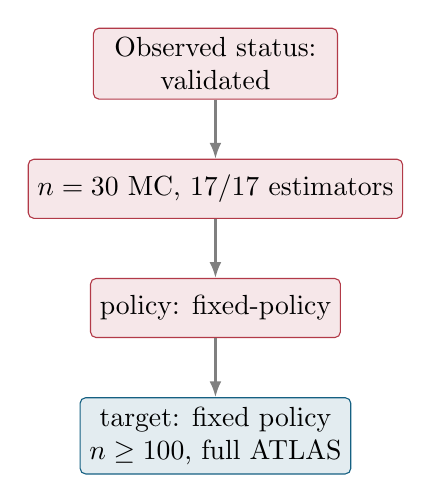
\begin{tikzpicture}[
  node distance=0.75cm,
  state/.style={draw, rounded corners=2pt, align=center, minimum width=3.1cm, minimum height=0.75cm},
  bad/.style={state, fill=ofbRed!12, draw=ofbRed},
  ok/.style={state, fill=ofbBlue!12, draw=ofbBlue},
  arr/.style={-{Latex[length=2mm]}, thick, color=gray}
]
\node[bad] (diag) {Observed status:\\\CurrentAtlasStatus};
\node[bad, below=of diag] (runs) {$n=\CurrentAtlasRuns$ MC, \CurrentAtlasEstimators/\CanonicalEstimatorCount\ estimators};
\node[bad, below=of runs] (policy) {policy: \CurrentAtlasPolicy};
\node[ok, below=of policy] (target) {target: fixed policy\\$n\ge 100$, full ATLAS};
\draw[arr] (diag) -- (runs);
\draw[arr] (runs) -- (policy);
\draw[arr] (policy) -- (target);
\end{tikzpicture}
\column{0.48\linewidth}
\begin{itemize}
  \item ATLAS smoke status: \textbf{\CurrentAtlasStatus}.
  \item Reported readiness issues: \textbf{\ReadinessIssueCount}.
  \item Full benchmark evidence requires complete sweeps, the canonical estimator set, fixed policy, and at least $n\ge30$.
  \item High-confidence qualification should repeat the same protocol with $n\ge100$.
\end{itemize}
\end{columns}
\artifact{artifacts/atlas-readiness-smoke/atlas\_readiness\_report.json}
\end{frame}

\begin{frame}{Experimental process and traceability}
\begin{center}
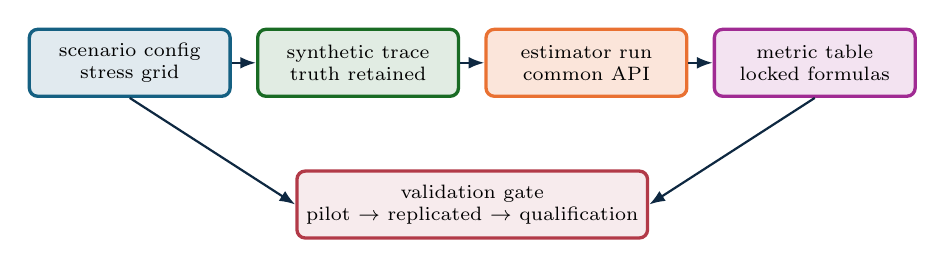
\begin{tikzpicture}[
  every node/.style={font=\scriptsize},
  lane/.style={draw, rounded corners=3pt, minimum width=2.55cm, minimum height=0.85cm, align=center, very thick},
  arr/.style={-{Latex[length=2mm]}, thick, color=ofbInk}
]
\node[lane, fill=ofbBlue!13, draw=ofbBlue] (cfg) at (0,0.8) {scenario config\\stress grid};
\node[lane, fill=ofbGreen!13, draw=ofbGreen] (trace) at (2.9,0.8) {synthetic trace\\truth retained};
\node[lane, fill=ofbGold!18, draw=ofbGold] (run) at (5.8,0.8) {estimator run\\common API};
\node[lane, fill=ofbViolet!13, draw=ofbViolet] (met) at (8.7,0.8) {metric table\\locked formulas};
\node[lane, fill=ofbRed!10, draw=ofbRed] (claim) at (4.35,-1.0) {validation gate\\pilot $\rightarrow$ replicated $\rightarrow$ qualification};
\draw[arr] (cfg) -- (trace);
\draw[arr] (trace) -- (run);
\draw[arr] (run) -- (met);
\draw[arr] (met.south) -- (claim.east);
\draw[arr] (cfg.south) -- (claim.west);
\end{tikzpicture}
\end{center}
\vspace{0.2em}
\begin{itemize}
  \item Each figure is derived from machine-readable CSV/JSON outputs generated by the same experimental pipeline.
  \item Traceability is part of the method: scenario definition, estimator outputs, metric tables, and readiness status are archived together.
\end{itemize}
\end{frame}

\fi
\begin{frame}{Full benchmark workflow}
\centering
\vspace{-0.35em}
\resizebox{0.985\textwidth}{!}{%
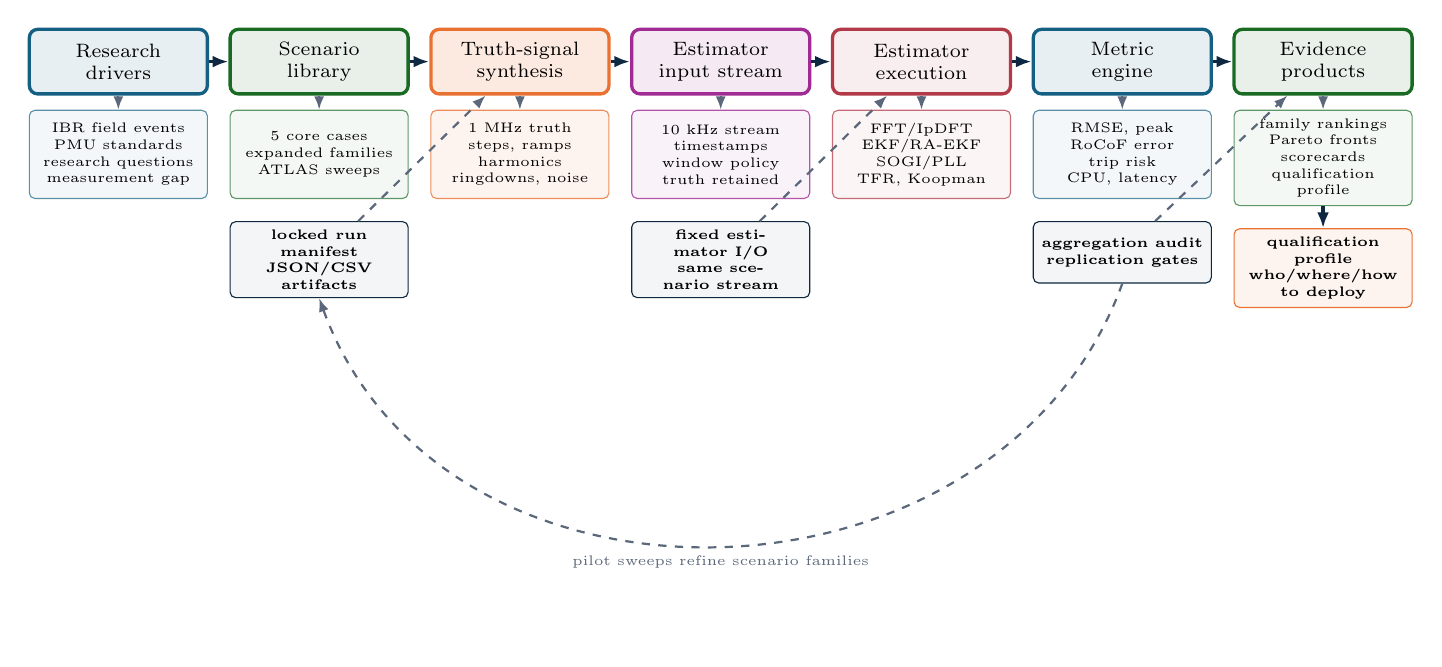
\begin{tikzpicture}[
  every node/.style={font=\scriptsize},
  stage/.style={draw, rounded corners=3pt, very thick, align=center, text width=2.05cm, minimum height=0.82cm, inner sep=3pt},
  detail/.style={draw, rounded corners=2pt, align=center, text width=2.05cm, minimum height=1.12cm, inner sep=3pt, font=\tiny},
  gate/.style={draw, rounded corners=2pt, align=center, text width=2.05cm, minimum height=0.78cm, inner sep=3pt, font=\tiny\bfseries},
  main/.style={-{Latex[length=2.0mm]}, very thick, color=ofbInk},
  aux/.style={-{Latex[length=1.7mm]}, thick, dashed, color=ofbMuted}
]
\node[stage, draw=ofbBlue, fill=ofbBlue!10] (drivers) at (0,2.8) {Research\\drivers};
\node[stage, draw=ofbGreen, fill=ofbGreen!10] (scenario) at (2.55,2.8) {Scenario\\library};
\node[stage, draw=ofbGold, fill=ofbGold!15] (truth) at (5.10,2.8) {Truth-signal\\synthesis};
\node[stage, draw=ofbViolet, fill=ofbViolet!10] (stream) at (7.65,2.8) {Estimator\\input stream};
\node[stage, draw=ofbRed, fill=ofbRed!9] (estimators) at (10.20,2.8) {Estimator\\execution};
\node[stage, draw=ofbBlue, fill=ofbBlue!10] (metrics) at (12.75,2.8) {Metric\\engine};
\node[stage, draw=ofbGreen, fill=ofbGreen!10] (evidence) at (15.30,2.8) {Evidence\\products};

\node[detail, draw=ofbBlue!70, fill=ofbBlue!5, below=0.18cm of drivers] (dDrivers)
{IBR field events\\PMU standards\\research questions\\measurement gap};
\node[detail, draw=ofbGreen!70, fill=ofbGreen!5, below=0.18cm of scenario] (dScenario)
{5 core cases\\expanded families\\ATLAS sweeps};
\node[detail, draw=ofbGold!80, fill=ofbGold!8, below=0.18cm of truth] (dTruth)
{1 MHz truth\\steps, ramps\\harmonics\\ringdowns, noise};
\node[detail, draw=ofbViolet!80, fill=ofbViolet!6, below=0.18cm of stream] (dStream)
{10 kHz stream\\timestamps\\window policy\\truth retained};
\node[detail, draw=ofbRed!75, fill=ofbRed!5, below=0.18cm of estimators] (dEstimators)
{FFT/IpDFT\\EKF/RA-EKF\\SOGI/PLL\\TFR, Koopman};
\node[detail, draw=ofbBlue!70, fill=ofbBlue!5, below=0.18cm of metrics] (dMetrics)
{RMSE, peak\\RoCoF error\\trip risk\\CPU, latency};
\node[detail, draw=ofbGreen!70, fill=ofbGreen!5, below=0.18cm of evidence] (dEvidence)
{family rankings\\Pareto fronts\\scorecards\\qualification profile};

\node[gate, draw=ofbInk, fill=ofbSoft, below=0.28cm of dScenario] (manifest)
{locked run manifest\\JSON/CSV artifacts};
\node[gate, draw=ofbInk, fill=ofbSoft, below=0.28cm of dStream] (contract)
{fixed estimator I/O\\same scenario stream};
\node[gate, draw=ofbInk, fill=ofbSoft, below=0.28cm of dMetrics] (audit)
{aggregation audit\\replication gates};
\node[gate, draw=ofbRust, fill=ofbRust!8, below=0.28cm of dEvidence] (profile)
{qualification profile\\who/where/how to deploy};

\draw[main] (drivers) -- (scenario);
\draw[main] (scenario) -- (truth);
\draw[main] (truth) -- (stream);
\draw[main] (stream) -- (estimators);
\draw[main] (estimators) -- (metrics);
\draw[main] (metrics) -- (evidence);

\foreach \a/\b in {drivers/dDrivers,scenario/dScenario,truth/dTruth,stream/dStream,estimators/dEstimators,metrics/dMetrics,evidence/dEvidence}
  \draw[aux] (\a) -- (\b);
\draw[aux] (manifest) -- (truth);
\draw[aux] (contract) -- (estimators);
\draw[aux] (audit) -- (evidence);
\draw[main] (dEvidence) -- (profile);
\draw[aux] (audit.south) to[out=-110,in=-70,looseness=1.15] node[below, font=\tiny, align=center, text=ofbMuted] {pilot sweeps refine scenario families} (manifest.south);
\end{tikzpicture}%
}
\end{frame}


\begin{frame}{Standard scenario results}
\scriptsize
\setlength{\tabcolsep}{3.5pt}
\renewcommand{\arraystretch}{1.12}
\begin{tabular}{>{\raggedright\arraybackslash}p{0.18\linewidth}rr|rr|rr}
\toprule
Method & \multicolumn{2}{c|}{Step +10\%} & \multicolumn{2}{c|}{Ramp +5 Hz/s} & \multicolumn{2}{c}{Modulation 2 Hz} \\
 & RMSE & Peak & RMSE & Peak & RMSE & Peak \\
\midrule
IpDFT & 0.00157 & 0.00741 & 0.0729 & 0.157 & 0.000281 & 0.000747 \\
TFT & 0.00210 & 0.0190 & 0.0726 & 0.127 & 0.000260 & 0.000781 \\
Koopman & \textbf{0.000207} & 0.00523 & 0.0549 & 0.0860 & \textbf{0.000212} & 0.00178 \\
\midrule
SRF-PLL & 0.000261 & 0.00132 & 0.142 & 0.354 & 0.000238 & \textbf{0.000441} \\
SOGI-FLL & 0.00900 & 0.0100 & 2.12 & 3.05 & 0.00900 & 0.0100 \\
\midrule
EKF & 0.000733 & 0.00857 & 0.0180 & 0.0631 & 0.00119 & 0.00265 \\
UKF & 0.000774 & 0.00851 & 0.0207 & 0.0657 & 0.00116 & 0.00271 \\
RA-EKF & 0.00231 & 0.0299 & \textbf{0.0113} & \textbf{0.0441} & 0.00476 & 0.0125 \\
\bottomrule
\end{tabular}
\vspace{0.30em}
\callout{Reading: the leader differs by scenario --- Koopman and SRF-PLL lead the step and modulation cases, while RA-EKF leads the ramp (0.0113 Hz RMSE). No method dominates all three standard cases.}
\artifact{Table III}
\end{frame}

\begin{frame}{Composite islanding: trip exposure under phase jump}
\begin{columns}[T,onlytextwidth]
\column{0.52\linewidth}
\begin{block}{Scenario D evidence}
\scriptsize
\begin{itemize}
  \item Instantaneous $+60^\circ$ phase jump with harmonic and interharmonic content.
  \item Windowed leakage: IpDFT reaches 0.481 Hz RMSE; TFT reaches 2.74 Hz.
  \item EKF/UKF incur $T_{\mathrm{trip}}=0.165$ s without phase-reset mechanisms.
  \item SRF-PLL is competitive on RMSE, 0.0645 Hz, with $T_{\mathrm{trip}}=0$.
\end{itemize}
\end{block}
\column{0.43\linewidth}
\begin{block}{RA-EKF result}
\scriptsize
\[
\mathrm{RMSE}=0.0695\ \mathrm{Hz}
\]
\[
T_{\mathrm{trip}}=0.6\ \mathrm{ms}
\]
\[
T_{\mathrm{trip}}:\ 165\ \mathrm{ms}\ \longrightarrow\ 0.6\ \mathrm{ms}
\]
\vspace{0.1em}
The gain comes from explicit $\dot\omega$ modeling plus event gating rather than post-hoc filtering.
\end{block}
\end{columns}
\vspace{0.15em}
{\scriptsize\color{ofbMuted}\textbf{Benchmark reading:} under this phase jump trip exposure spans 0--165 ms across methods; SRF-PLL and RA-EKF keep it near zero, while windowed and plain EKF/UKF methods do not.}
\end{frame}

\begin{frame}{Multi-event trip-risk}
\scriptsize
\setlength{\tabcolsep}{7pt}
\renewcommand{\arraystretch}{1.14}
\begin{center}
\begin{tabular}{>{\bfseries\raggedright\arraybackslash}p{0.20\linewidth}rrr}
\toprule
Method & RMSE [Hz] & $T_{\mathrm{trip}}$ [s] & CPU [$\mu$s] \\
\midrule
RA-EKF & 0.511 & 0.141 & 54 \\
EKF & 0.789 & \textbf{0.118} & 18 \\
Koopman & \textbf{0.476} & 0.137 & 85 \\
UKF & 0.792 & 0.119 & 139 \\
SRF-PLL & 0.400 & 0.471 & 11 \\
IpDFT & 1.36 & 0.335 & 48 \\
SOGI-FLL & 0.568 & 0.422 & 25 \\
\bottomrule
\end{tabular}
\end{center}
\vspace{0.30em}
\begin{columns}[T,onlytextwidth]
\column{0.48\linewidth}
\begin{block}{Main reading}
\small
RA-EKF sits in the practical protection region: low trip exposure, moderate RMSE, and embedded-feasible CPU.
\end{block}
\column{0.47\linewidth}
\begin{block}{Scalar ranking failure}
\small
SRF-PLL has low CPU and good RMSE but much higher $T_{\mathrm{trip}}$; EKF has lower $T_{\mathrm{trip}}$ but worse RMSE; Koopman is accurate but costlier.
\end{block}
\end{columns}
\artifact{Table IV}
\end{frame}

\begin{frame}{Trip-risk evidence: core stress cases}
\begin{columns}[T,onlytextwidth]
\column{0.68\linewidth}
\centering
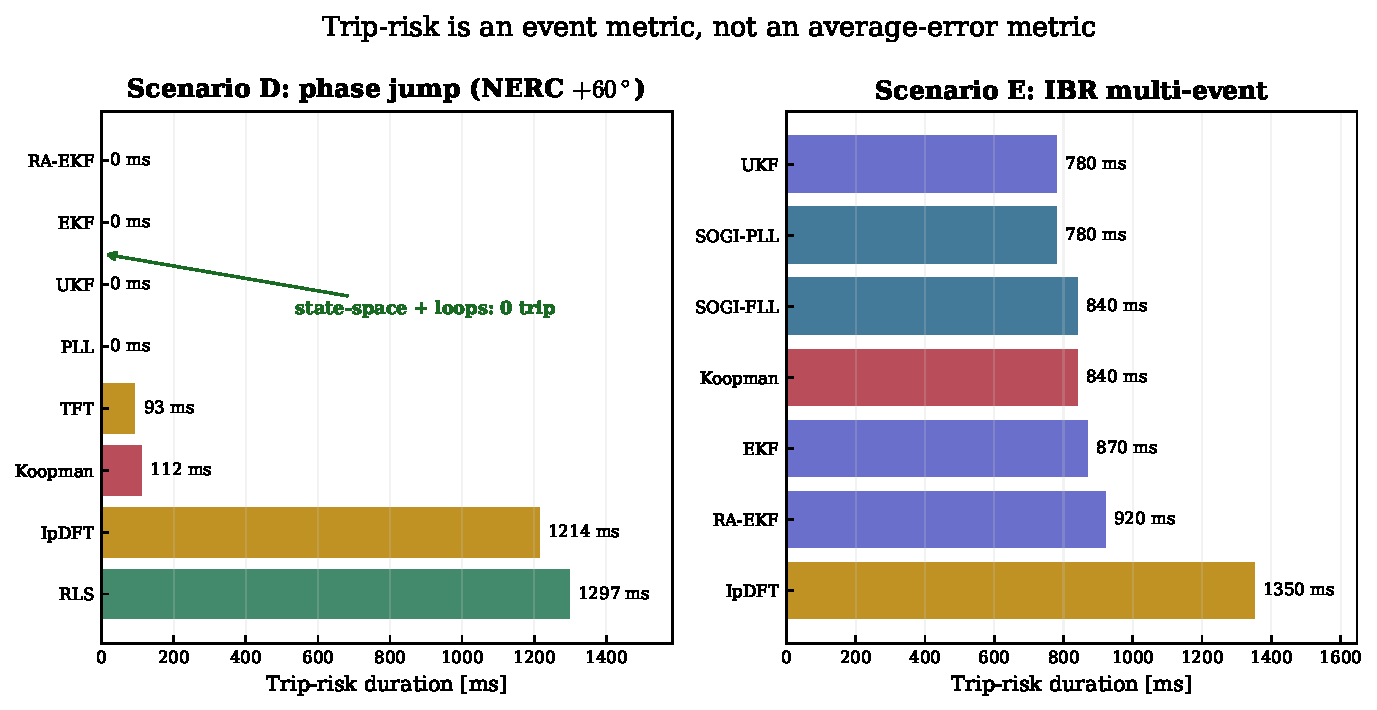
\includegraphics[width=\linewidth,height=0.58\textheight,keepaspectratio]{figures/core_trip_risk_comparison.pdf}
\column{0.28\linewidth}
\begin{block}{Result reading}
\scriptsize
\begin{itemize}
  \item Scenario D exposes phase-reset behavior: RA-EKF reduces EKF exposure from 165 ms to 0.6 ms.
  \item Scenario E is multi-objective: RMSE and trip-risk select different methods.
  \item SRF-PLL is strong in Scenario D but reaches 471 ms in Scenario E.
\end{itemize}
\end{block}
{\scriptsize\color{ofbMuted}\textbf{Result:} $T_{\mathrm{trip}}$ separates protection exposure from average error.}
\end{columns}
\end{frame}

\begin{frame}{Result comparison: winners depend on the question}
\scriptsize
\setlength{\tabcolsep}{5pt}
\renewcommand{\arraystretch}{1.16}
\begin{center}
\resizebox{0.98\linewidth}{!}{%
\begin{tabular}{>{\bfseries\raggedright\arraybackslash}p{0.22\linewidth}>{\raggedright\arraybackslash}p{0.23\linewidth}>{\raggedright\arraybackslash}p{0.20\linewidth}>{\raggedright\arraybackslash}p{0.27\linewidth}}
\toprule
Question & Best-supported answer & Evidence & Boundary \\
\midrule
Clean step/modulation accuracy & Koopman and SRF-PLL are strongest point cases & Step RMSE 0.000207 Hz; modulation peak 0.000441 Hz & Not enough for islanding or multi-event survival \\
Ramp and RoCoF tracking & RA-EKF is strongest in the standard ramp & Ramp RMSE 0.0113 Hz & Not a universal RMSE winner \\
Composite islanding exposure & RA-EKF removes long EKF exposure & 0.6 ms vs 165 ms for EKF & SRF-PLL is also strong in this specific phase-jump case \\
Multi-event RMSE & Koopman and SRF-PLL are competitive & 0.476 Hz and 0.400 Hz & RMSE hides trip-risk and compute trade-offs \\
Embedded protection feasibility & SRF-PLL, EKF, SOGI-FLL, RA-EKF remain plausible & 11--54 $\mu$s/sample range & Python timing is a software-cost proxy \\
\bottomrule
\end{tabular}%
}
\end{center}
\vspace{0.28em}
\callout{Selection changes with event family, objective metric, and compute envelope. A single leaderboard hides the deployment trade-off.}
\end{frame}

\begin{frame}{Computational feasibility}
\scriptsize
\setlength{\tabcolsep}{5pt}
\renewcommand{\arraystretch}{1.12}
\begin{columns}[T,onlytextwidth]
\column{0.50\linewidth}
\begin{tabular}{>{\bfseries\raggedright\arraybackslash}p{0.27\linewidth}rcc}
\toprule
Method & Time/sample & Class & Target \\
\midrule
SRF-PLL & 11 $\mu$s & P2 & MCU \\
EKF & 18 $\mu$s & P1 & DSP \\
TFT & 25 $\mu$s & P1 & DSP \\
SOGI-FLL & 25 $\mu$s & P2 & MCU/DSP \\
IpDFT & 48 $\mu$s & M1 & DSP/FPGA \\
RA-EKF & \textbf{54 $\mu$s} & \textbf{P1} & \textbf{DSP/FPGA} \\
Koopman & 85 $\mu$s & M1 & CPU \\
UKF & 139 $\mu$s & P1 & high-perf CPU \\
PI-GRU & $\approx$136{,}000 $\mu$s & -- & GPU only \\
\bottomrule
\end{tabular}
\column{0.46\linewidth}
\begin{block}{Deployment interpretation}
\small
The Python baseline separates feasible estimator families from clearly prohibitive ones; hardware latency requires platform timing.
\end{block}
\begin{block}{Key comparison}
\small
RA-EKF is roughly three times EKF cost in Python but remains below the millisecond scale by a wide margin; PI-GRU is retained as a computational reference outside embedded protection targets.
\end{block}
\end{columns}
\artifact{Table V}
\end{frame}

\begin{frame}{Event responses}
\centering
\vspace{-0.25em}
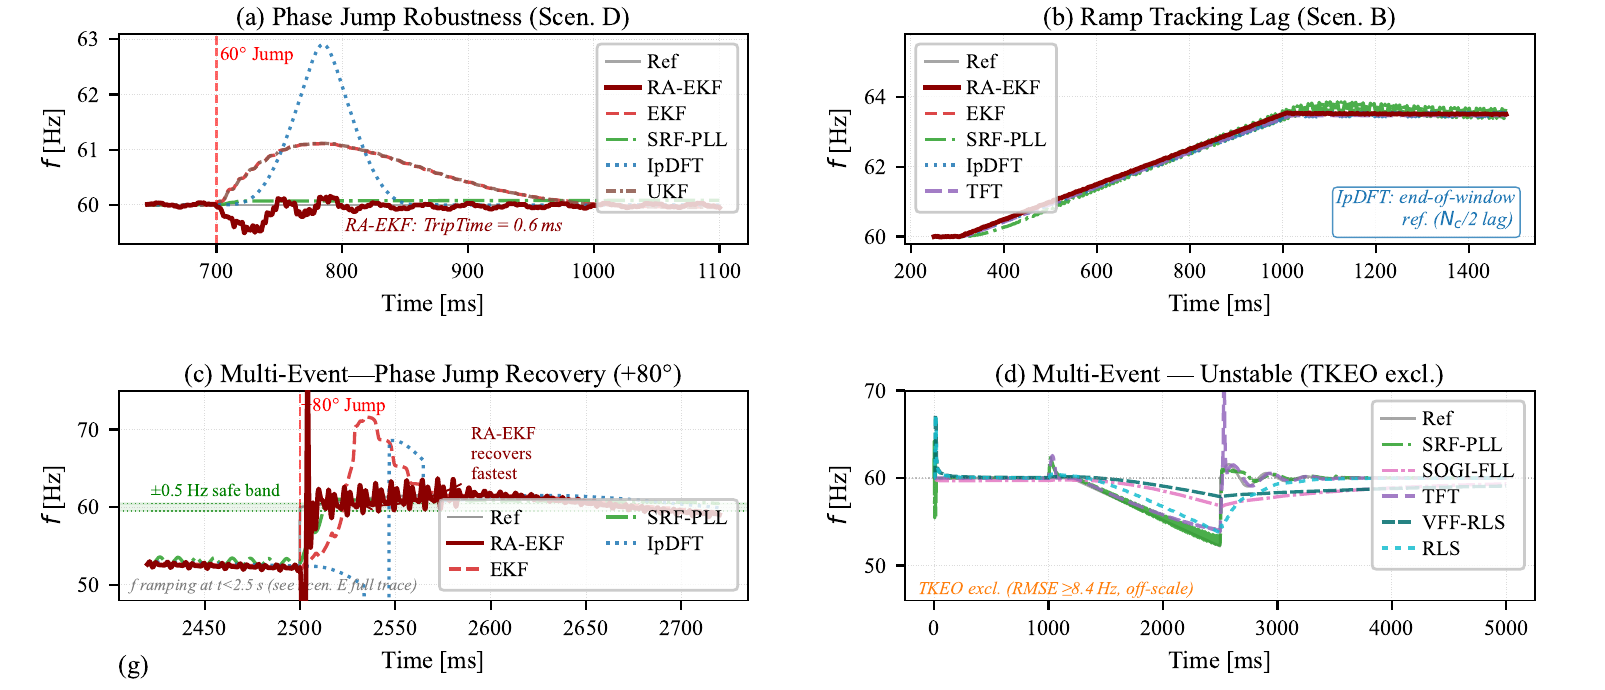
\includegraphics[width=0.98\paperwidth,height=0.78\textheight,keepaspectratio]{figures/doc1_fig2_ad.png}
\end{frame}

\begin{frame}{Deployment limits}
\begin{columns}[T,onlytextwidth]
\column{0.56\linewidth}
\centering
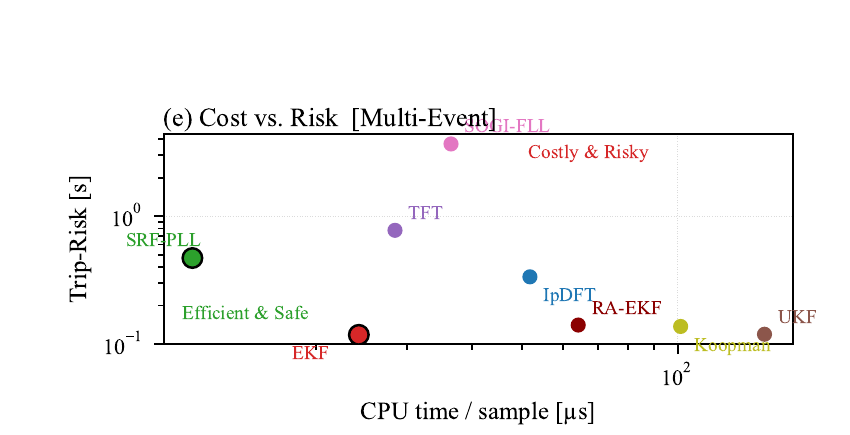
\includegraphics[width=0.84\linewidth]{figures/doc1_fig2_e_costrisk.png}
\vspace{0.15em}
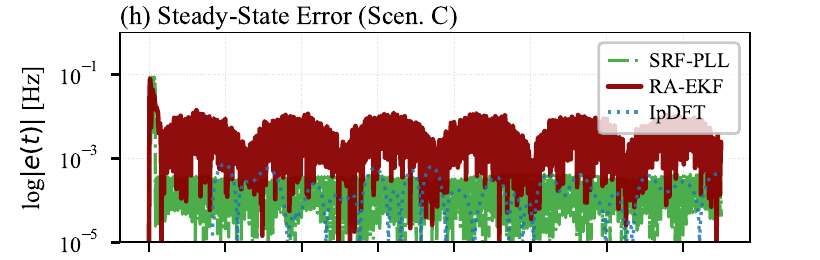
\includegraphics[width=0.84\linewidth]{figures/doc1_fig2_h_error.png}
\column{0.40\linewidth}
\begin{exampleblock}{Dashboard reading}
\begin{itemize}
\setlength\itemsep{0.22em}
\item Deployment risk requires RMSE, trip exposure, settling, and delay.
\item Trip-risk exposes the cost of estimator transients in composite events.
\item Windowed methods can be accurate but delayed.
\item RA-EKF occupies the main protection-oriented trade-off point.
\end{itemize}
\end{exampleblock}
\end{columns}
\end{frame}

\begin{frame}{Balance profile}
\begin{columns}[T,onlytextwidth]
\column{0.58\linewidth}
\centering
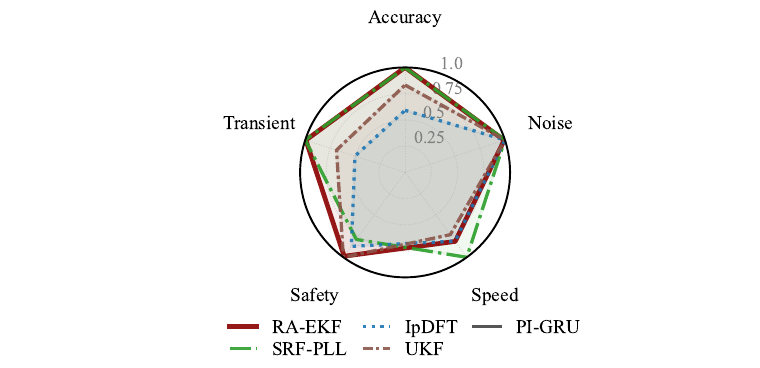
\includegraphics[width=\linewidth]{figures/doc1_fig2_f_radar.png}
\column{0.38\linewidth}
\begin{block}{Radar profile}
\begin{itemize}
\setlength\itemsep{0.32em}
\item Accuracy, speed, noise immunity, safety, and transient behavior are conflicting axes.
\item RA-EKF is selected for event-rich protection use cases.
\item SRF-PLL remains valuable when cost and simplicity dominate.
\item IpDFT is attractive where observation delay is acceptable.
\end{itemize}
\end{block}
\end{columns}
\end{frame}

\begin{frame}{Compliance heatmap: why standard tests are insufficient}
\scriptsize
\setlength{\tabcolsep}{5pt}
\renewcommand{\arraystretch}{1.08}
\begin{center}
\begin{tabular}{>{\bfseries\raggedright\arraybackslash}p{0.18\linewidth}ccccc}
\toprule
Method & Step & Ramp & Mod & Isl & Multi \\
\midrule
PI-GRU & \cellcolor{ofbRed!22}F & \cellcolor{ofbRed!22}F & \cellcolor{ofbRed!22}F & \cellcolor{ofbRed!22}F & \cellcolor{ofbRed!22}F \\
Koopman & \cellcolor{ofbGreen!25}P & \cellcolor{ofbRed!22}F & \cellcolor{ofbGreen!25}P & \cellcolor{ofbRed!22}F & \cellcolor{ofbRed!22}F \\
TFT & \cellcolor{ofbGreen!25}P & \cellcolor{ofbRed!22}F & \cellcolor{ofbGreen!25}P & \cellcolor{ofbRed!22}F & \cellcolor{ofbRed!22}F \\
IpDFT & \cellcolor{ofbGreen!25}P & \cellcolor{ofbRed!22}F & \cellcolor{ofbGreen!25}P & \cellcolor{ofbRed!22}F & \cellcolor{ofbRed!22}F \\
SOGI-FLL & \cellcolor{ofbGreen!25}P & \cellcolor{ofbRed!22}F & \cellcolor{ofbGreen!25}P & \cellcolor{ofbGreen!25}P & \cellcolor{ofbRed!22}F \\
SRF-PLL & \cellcolor{ofbGreen!25}P & \cellcolor{ofbRed!22}F & \cellcolor{ofbGreen!25}P & \cellcolor{ofbRed!22}F & \cellcolor{ofbRed!22}F \\
EKF & \cellcolor{ofbGreen!25}P & \cellcolor{ofbGreen!25}P & \cellcolor{ofbGreen!25}P & \cellcolor{ofbRed!22}F & \cellcolor{ofbRed!22}F \\
UKF & \cellcolor{ofbGreen!25}P & \cellcolor{ofbGreen!25}P & \cellcolor{ofbGreen!25}P & \cellcolor{ofbRed!22}F & \cellcolor{ofbRed!22}F \\
RA-EKF & \cellcolor{ofbGreen!25}P & \cellcolor{ofbGreen!25}P & \cellcolor{ofbGreen!25}P & \cellcolor{ofbGold!30}F* & \cellcolor{ofbRed!22}F \\
\bottomrule
\end{tabular}
\end{center}
\vspace{0.30em}
\callout{Several methods pass the standard-style Step/Ramp/Mod columns and still fail under composite islanding or multi-event IBR stress. Standard tests leave IBR event readiness partially untested.}
\end{frame}

\begin{frame}{Empirical claims}
\begin{columns}[T,onlytextwidth]
\column{0.48\linewidth}
\begin{block}{Protection behavior}
\scriptsize
\textbf{An explicit dynamic state plus event gating cuts trip exposure.}\\
Scenario D gives $T_{\mathrm{trip}}=0.6$ ms for the RA-EKF variant versus 0.165 s for the plain EKF.
\end{block}
\begin{block}{Standard-test limitation}
\scriptsize
\textbf{Simple-case pass/fail leaves event readiness unresolved.}\\
The heatmap shows methods that pass Step/Ramp/Mod but fail islanding or multi-event IBR stress.
\end{block}
\column{0.48\linewidth}
\begin{block}{Metric disagreement}
\scriptsize
\textbf{RMSE, trip-risk, and CPU select different winners.}\\
Table IV separates Koopman/SRF-PLL accuracy, EKF/UKF trip exposure, and low-cost loop/filter deployment.
\end{block}
\begin{block}{Deployability}
\scriptsize
\textbf{Feasibility changes the accuracy ranking.}\\
RA-EKF remains in a 54 $\mu$s/sample software-cost regime; PI-GRU is retained as a computational reference outside relay-class timing.
\end{block}
\end{columns}
\vspace{0.15em}
{\scriptsize\color{ofbMuted}\textbf{Guardrail:} report scenario, metric, and compute envelope before naming a preferred estimator.}
\end{frame}

\begin{frame}{Composite IBR sequence: why it is hardest}
\begin{columns}[T,onlytextwidth]
\column{0.48\linewidth}
\begin{block}{Scenario E stress components}
\small
\begin{itemize}
  \item Harmonic-rich steady state: 5th at 5\%, 7th at 3\%, low interharmonics.
  \item $+40^\circ$ phase jump.
  \item $-6$ Hz/s RoCoF segment.
  \item $+80^\circ$ phase jump with ringdown.
  \item Sparse impulsive noise.
\end{itemize}
\end{block}
\column{0.47\linewidth}
\begin{block}{Standard-test gap}
\small
\begin{itemize}
  \item The estimator sees a nonstationary waveform with stacked disturbances.
  \item Spectral leakage, loop re-lock, state-model mismatch, and recovery delay occur together.
  \item A method can be good on RMSE and still undesirable on trip exposure or CPU.
\end{itemize}
\end{block}
\end{columns}
\vspace{0.35em}
\callout{Once composite stress is shown to matter, ATLAS sweeps each stress component systematically instead of treating the multi-event case as a single aggregate disturbance.}
\end{frame}

\begin{frame}{Expanded stress analysis}
\extendedresultsbanner
\begin{columns}[T,onlytextwidth]
\column{0.48\linewidth}
\begin{block}{Core experiment}
\small
\begin{itemize}
  \item 9 principal estimators + 2 legacy baselines.
  \item 5 scenarios: A--E.
  \item Standard, islanding, multi-event, and CPU results.
  \item RA-EKF supplies the tested estimator mechanism.
\end{itemize}
\end{block}
\column{0.47\linewidth}
\begin{block}{Expanded benchmark}
\small
\begin{itemize}
  \item 18-estimator, 32-scenario, 10-family diagnostic sweep.
  \item Pilot Monte Carlo ($n=5$), per-scenario tuned --- diagnostic-grade.
  \item ATLAS severity curves and harmonic sweeps.
  \item Used to test sensitivity, scaling, and estimator-family stability.
\end{itemize}
\end{block}
\end{columns}
\vspace{0.25em}
\callout{The expanded benchmark scales the same measurement question across more event families, estimator types, and Monte Carlo replications.}
\end{frame}

\begin{frame}{Expanded benchmark: family winners}
\extendedresultsbanner
\scriptsize
\setlength{\tabcolsep}{3.5pt}
\renewcommand{\arraystretch}{1.08}
\begin{tabular}{>{\raggedright\arraybackslash}p{0.20\linewidth}c>{\raggedright\arraybackslash}p{0.18\linewidth}>{\raggedright\arraybackslash}p{0.18\linewidth}>{\raggedright\arraybackslash}p{0.23\linewidth}}
\toprule
\textbf{Family} & \textbf{Count} & \textbf{RMSE leader} & \textbf{RMSE} & \textbf{Trip-risk leader} \\
\midrule
IEEE ramps & 9 & SOGI-PLL & 19.4 mHz & 0 s, multiple estimators \\
Magnitude steps & 7 & EKF & 0.388 mHz & 0 s, multiple estimators \\
Modulation & 3 & RA-EKF & 17.8 mHz & 0 s, multiple estimators \\
Phase jumps & 3 & SOGI-FLL & 174 mHz & ZCD, 0.0194 s \\
OOB interference & 1 & EKF & 13.6 mHz & EKF / RA-EKF, 0 s \\
IBR harmonics & 3 & EKF & 70.5 mHz & TFT / Prony, 0.00947 s \\
IBR ringdown & 5 & UKF & 313 mHz & ESPRIT, 0.0989 s \\
IBR multi-event & 1 & PLL & 173.5 mHz & IpDFT, 0.0439 s \\
\bottomrule
\end{tabular}
\vspace{0.25em}
\callout{The expanded sweep confirms the central pattern: estimator rankings depend on disturbance family and metric target.}
\end{frame}

\begin{frame}{ATLAS severity analysis}
\atlaspreviewbanner
\begin{center}
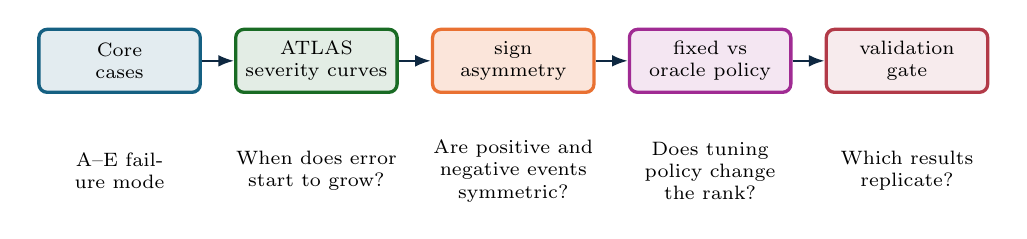
\begin{tikzpicture}[
  every node/.style={font=\scriptsize},
  box/.style={draw, rounded corners=3pt, very thick, align=center, minimum width=2.05cm, minimum height=0.80cm},
  arr/.style={-{Latex[length=2mm]}, thick, color=ofbInk}
]
\node[box, fill=ofbBlue!12, draw=ofbBlue] (paper) at (0,1.15) {Core\\cases};
\node[box, fill=ofbGreen!12, draw=ofbGreen] (sev) at (2.5,1.15) {ATLAS\\severity curves};
\node[box, fill=ofbGold!18, draw=ofbGold] (sign) at (5.0,1.15) {sign\\asymmetry};
\node[box, fill=ofbViolet!12, draw=ofbViolet] (policy) at (7.5,1.15) {fixed vs\\oracle policy};
\node[box, fill=ofbRed!10, draw=ofbRed] (gate) at (10.0,1.15) {validation\\gate};
\draw[arr] (paper) -- (sev);
\draw[arr] (sev) -- (sign);
\draw[arr] (sign) -- (policy);
\draw[arr] (policy) -- (gate);
\node[align=center, text width=2.1cm] at (0,-0.25) {A--E failure mode};
\node[align=center, text width=2.1cm] at (2.5,-0.25) {When does error start to grow?};
\node[align=center, text width=2.1cm] at (5.0,-0.25) {Are positive and negative events symmetric?};
\node[align=center, text width=2.1cm] at (7.5,-0.25) {Does tuning policy change the rank?};
\node[align=center, text width=2.1cm] at (10.0,-0.25) {Which results replicate?};
\end{tikzpicture}
\end{center}
\vspace{0.35em}
\callout{ATLAS maps where estimator behavior changes with severity, sign, tuning policy, and replication depth.}
\artifact{docs/ATLAS\_PIPELINE.md; docs/ATLAS\_METHOD\_AUDIT.md}
\end{frame}

\begin{frame}{Dynamic accuracy ranking}
\atlaspreviewbanner
\begin{center}
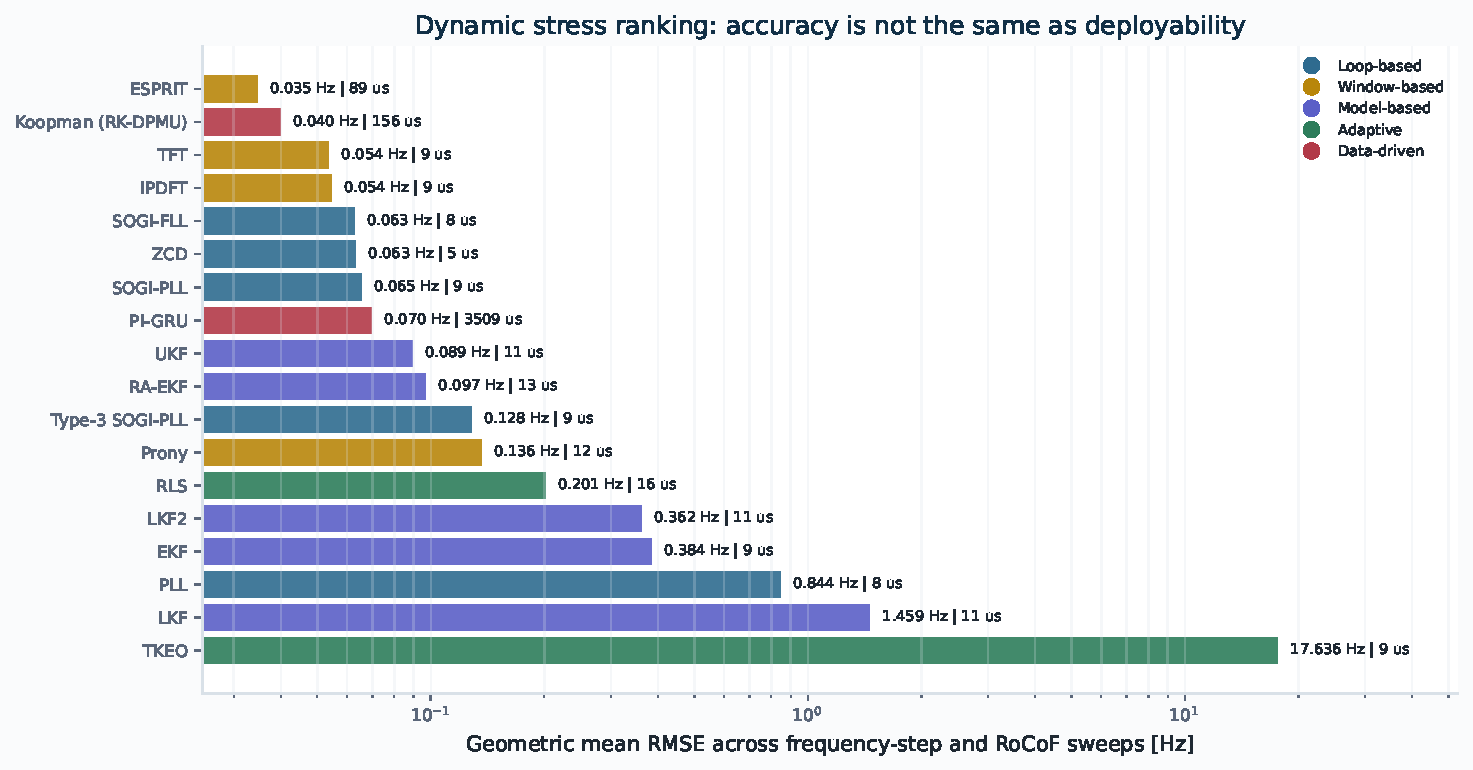
\includegraphics[width=0.94\linewidth,height=0.70\textheight,keepaspectratio]{figures/dynamic_composite_rank.pdf}
\end{center}
\end{frame}

\ifbackupframes
\begin{frame}{Frequency RMSE: leading estimators}
\atlaspreviewbanner
\begin{center}
\scriptsize
\resizebox{0.90\linewidth}{!}{\DynamicTopTable}
\end{center}
\vspace{0.45em}
\begin{itemize}
  \item ESPRIT and Koopman provide the lowest geometric dynamic RMSE in the analyzed runs.
  \item TFT, IpDFT, SOGI-FLL, ZCD, and SOGI-PLL form a competitive low-cost tier.
  \item PI-GRU is accurate but its CPU cost changes its deployment interpretation.
\end{itemize}
\end{frame}
\fi

\begin{frame}{Sensitivity to disturbance severity}
\atlaspreviewbanner
\begin{center}
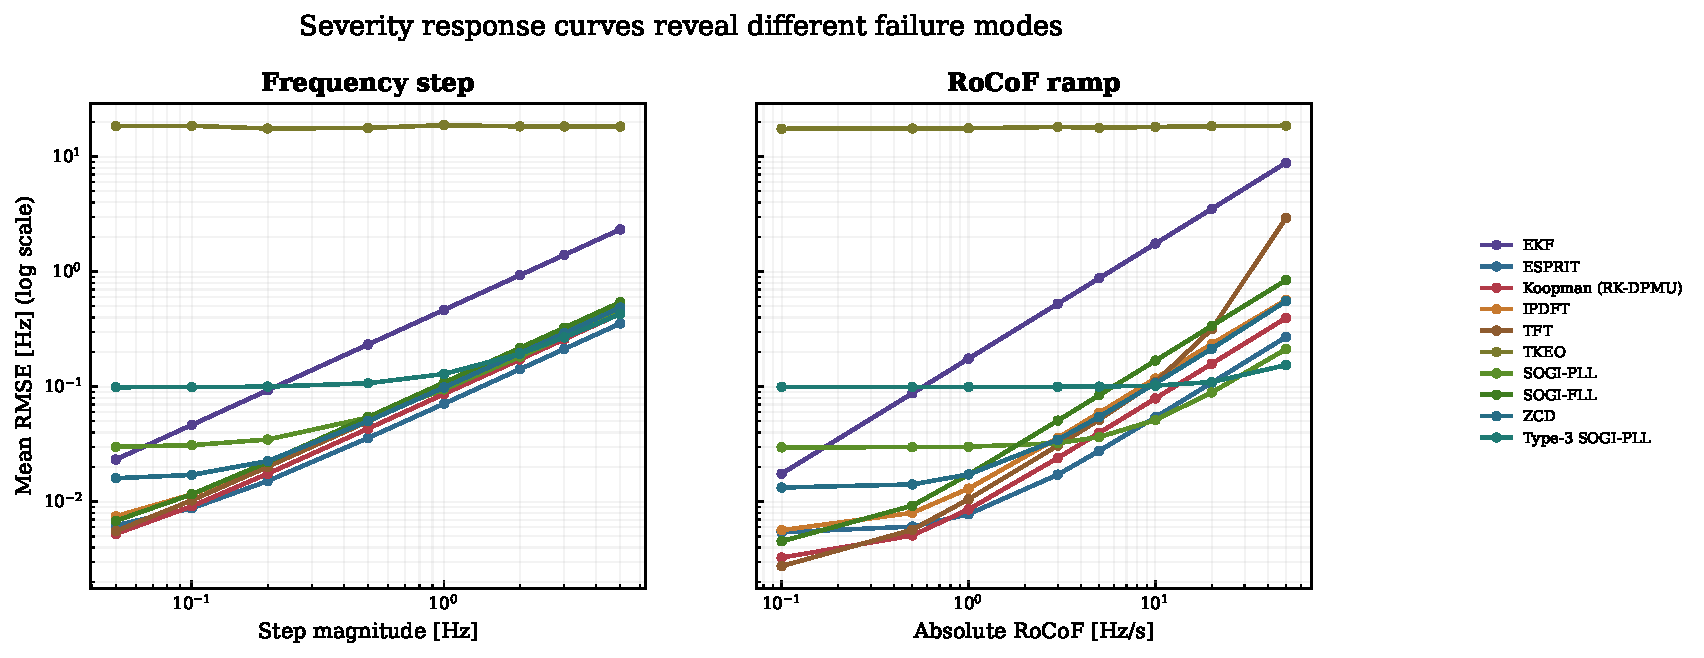
\includegraphics[width=0.94\linewidth,height=0.70\textheight,keepaspectratio]{figures/dynamic_sensitivity_curves.pdf}
\end{center}
\end{frame}

\ifbackupframes
\begin{frame}{Interpreting sensitivity curves}
\atlaspreviewbanner
\begin{columns}[T,onlytextwidth]
\column{0.46\linewidth}
\begin{itemize}
  \item Power-law-like growth indicates a measurable stress response.
  \item A nearly flat curve can still mean high baseline error.
  \item Type-3 SOGI-PLL has weak average frequency RMSE but favorable worst-case behavior under selected RoCoF conditions.
\end{itemize}
\column{0.50\linewidth}
\begin{center}
\scriptsize
\resizebox{\linewidth}{!}{\RegimeDiagnosticTable}
\end{center}
\end{columns}
\vspace{0.35em}
\callout{Classify curves as stable-flat, failed-flat, monotone-sensitive, or sign-asymmetric before interpreting aggregate error.}
\end{frame}

\begin{frame}{Frequency and RoCoF disagree}
\atlaspreviewbanner
\begin{center}
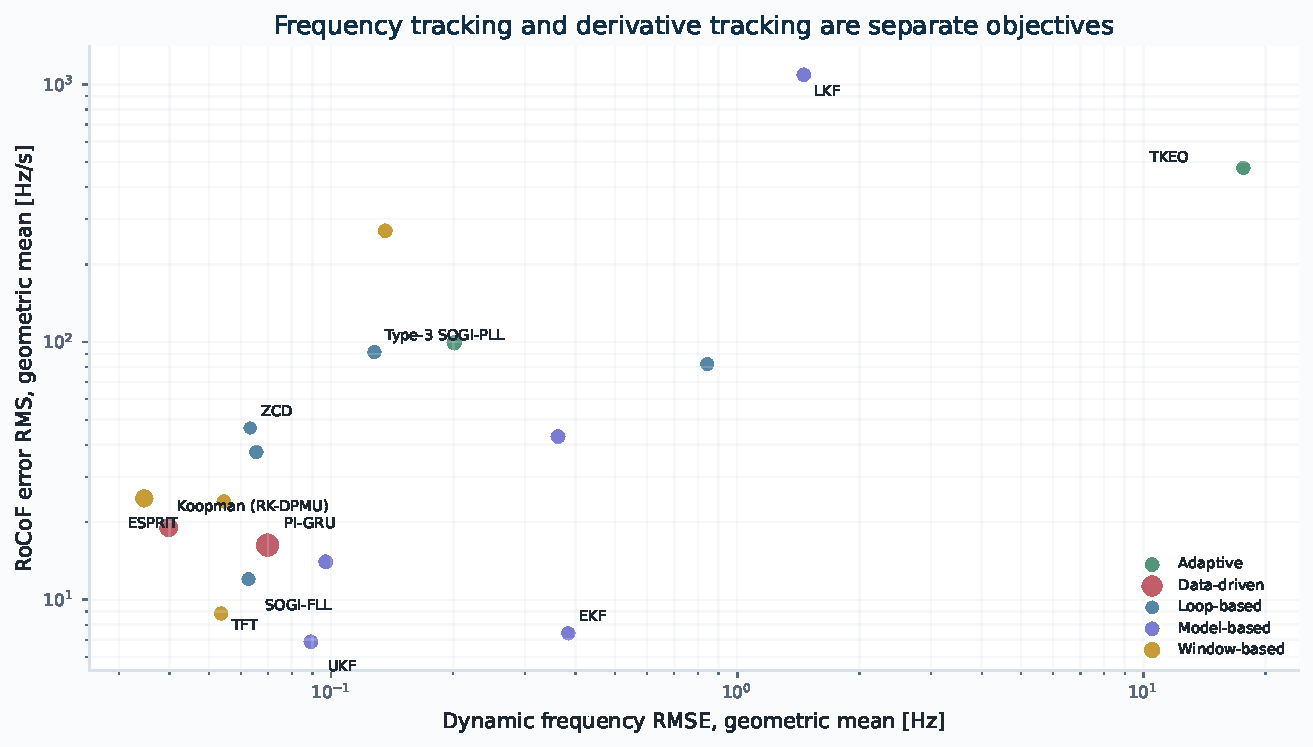
\includegraphics[width=0.94\linewidth,height=0.70\textheight,keepaspectratio]{figures/accuracy_rfe_tradeoff.pdf}
\end{center}
\end{frame}
\fi

\begin{frame}{Rank shift when the metric changes}
\atlaspreviewbanner
\begin{center}
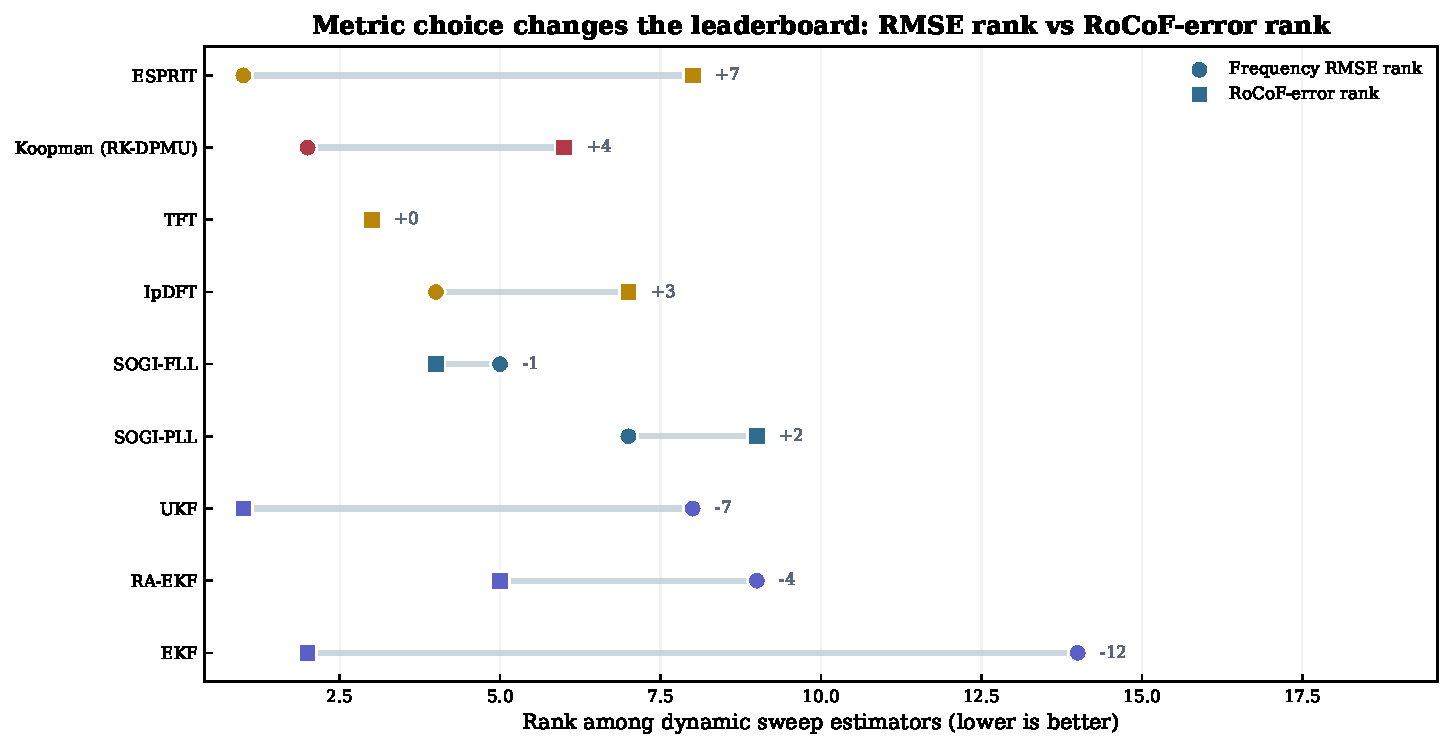
\includegraphics[width=0.98\linewidth,height=0.66\textheight,keepaspectratio]{figures/metric_rank_shift.pdf}
\end{center}
\end{frame}

\ifbackupframes
\begin{frame}{Derivative tracking: top RoCoF results}
\atlaspreviewbanner
\begin{center}
\scriptsize
\resizebox{0.90\linewidth}{!}{\RfeTopTable}
\end{center}
\vspace{0.45em}
\begin{itemize}
  \item UKF, EKF, TFT, SOGI-FLL, and RA-EKF move upward when the metric is RoCoF error.
  \item ESPRIT and Koopman remain competitive, but they no longer dominate the ranking.
  \item RoCoF error needs its own ranking because derivative performance has a separate order from frequency RMSE.
\end{itemize}
\end{frame}
\fi

\begin{frame}{CPU--accuracy Pareto analysis}
\atlaspreviewbanner
\begin{center}
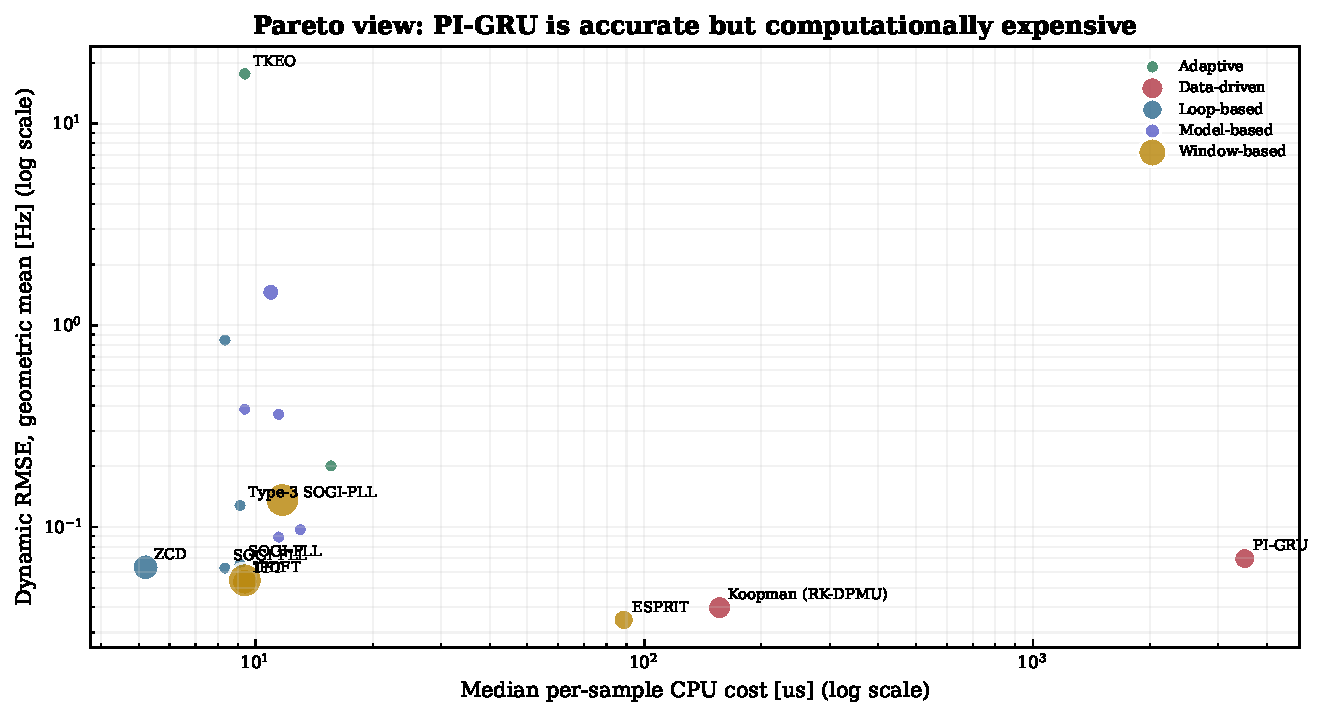
\includegraphics[width=0.94\linewidth,height=0.70\textheight,keepaspectratio]{figures/cpu_accuracy_pareto.pdf}
\end{center}
\end{frame}

\ifbackupframes
\begin{frame}{Interpreting the Pareto front}
\atlaspreviewbanner
\begin{columns}[T,onlytextwidth]
\column{0.48\linewidth}
\begin{block}{Low-cost online monitoring}
ZCD, SOGI-FLL, SOGI-PLL, TFT, and IpDFT sit close to the low-cost frontier, with window latency as the main caveat for TFT/IpDFT.
\end{block}
\begin{block}{High dynamic accuracy}
ESPRIT and Koopman are strong candidates when additional compute and latency are acceptable.
\end{block}
\column{0.48\linewidth}
\begin{block}{Data-driven estimation}
PI-GRU is empirically competitive in RMSE but requires a hardware and batching argument because of CPU cost.
\end{block}
\begin{block}{Methodological consequence}
A single leaderboard would hide deployment constraints that matter in grid instrumentation.
\end{block}
\end{columns}
\end{frame}
\fi

\begin{frame}{Harmonic-stress response}
\atlaspreviewbanner
\begin{center}
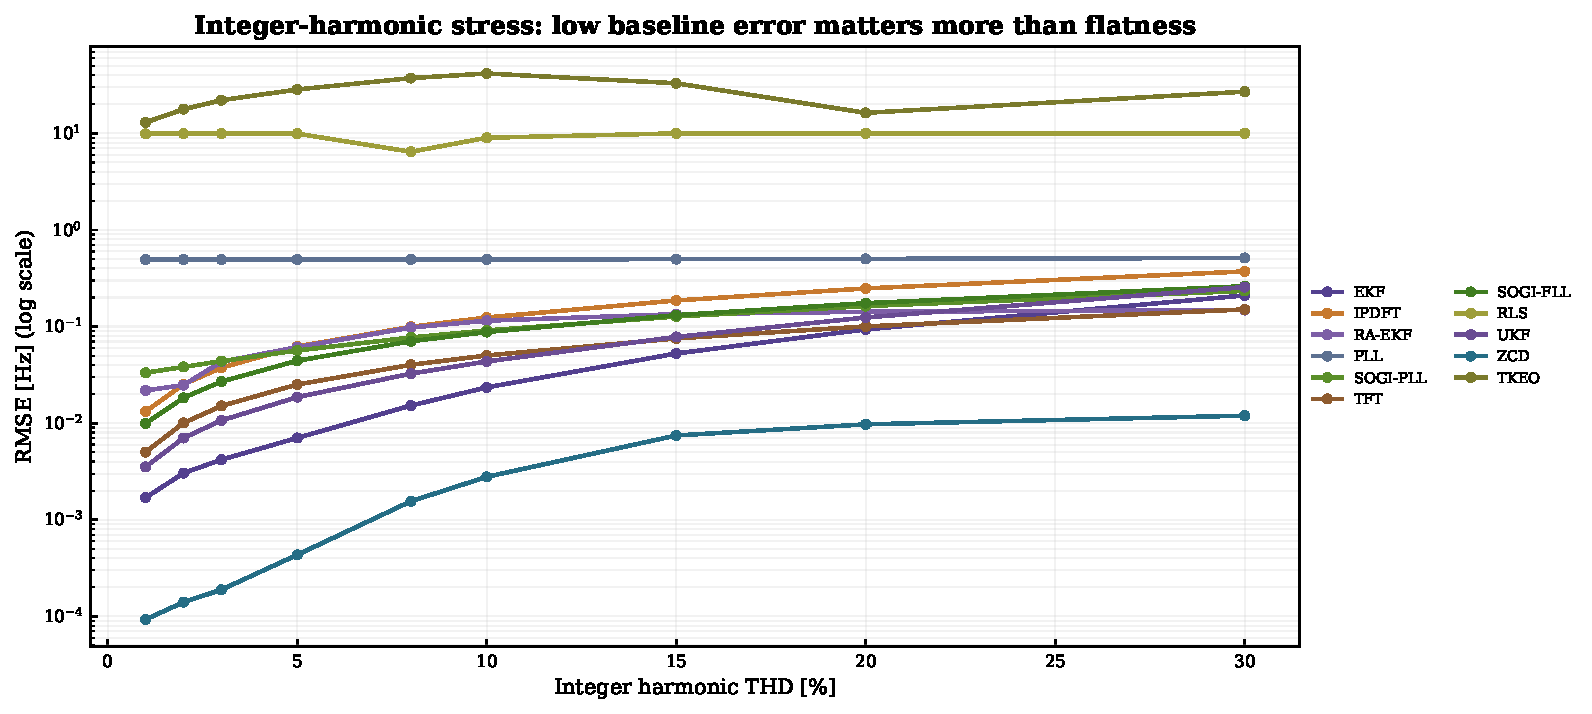
\includegraphics[width=0.94\linewidth,height=0.70\textheight,keepaspectratio]{figures/harmonics_sensitivity.pdf}
\end{center}
\end{frame}

\ifbackupframes
\begin{frame}{Harmonic sweep interpretation}
\atlaspreviewbanner
\begin{center}
\scriptsize
\resizebox{0.78\linewidth}{!}{\HarmonicsEndpointTable}
\end{center}
\vspace{0.35em}
\begin{itemize}
  \item ZCD is unexpectedly strong under isolated integer-harmonic stress in the pilot harmonic run.
  \item Generalization to interharmonics, noise, IBR-rich events, or mixed disturbances requires additional runs.
  \item RA-EKF, TFT, EKF, SOGI-PLL, and UKF remain secondary candidates for harmonic stress.
  \item Low slope must be read with baseline RMSE; both values are needed.
\end{itemize}
\end{frame}
\fi


\begin{frame}{Reading the evidence: three levels}
\begin{columns}[T,onlytextwidth]
\column{0.50\linewidth}
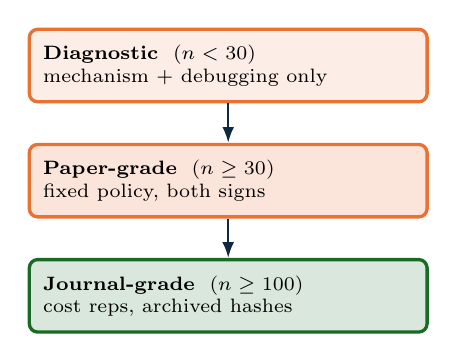
\begin{tikzpicture}[
  every node/.style={font=\scriptsize},
  lvl/.style={draw, rounded corners=3pt, very thick, align=left, text width=4.7cm, minimum height=0.92cm, inner sep=5pt},
  arr/.style={-{Latex[length=2mm]}, thick, color=ofbInk}
]
\node[lvl, fill=ofbRust!12, draw=ofbRust] (d) at (0,0) {\textbf{Diagnostic}\ \ ($n<30$)\\mechanism + debugging only};
\node[lvl, fill=ofbGold!18, draw=ofbGold, below=0.5cm of d] (p) {\textbf{Paper-grade}\ \ ($n\ge30$)\\fixed policy, both signs};
\node[lvl, fill=ofbGreen!16, draw=ofbGreen, below=0.5cm of p] (j) {\textbf{Journal-grade}\ \ ($n\ge100$)\\cost reps, archived hashes};
\draw[arr] (d) -- (p);
\draw[arr] (p) -- (j);
\end{tikzpicture}
\column{0.46\linewidth}
\begin{block}{Where this talk sits}
\small
\begin{itemize}
  \item Core 5-scenario results: tuned comparison evidence.
  \item Expanded sweep + ATLAS: \textbf{diagnostic pilots} ($n=5$ / $n=1$).
  \item They reveal \emph{mechanisms} and rank \emph{hypotheses} for the paper-grade campaign.
\end{itemize}
\end{block}
\callout{Every expanded/ATLAS result that follows is a pilot. The contribution is the benchmark and what it exposes --- not a final leaderboard.}
\end{columns}
\end{frame}

\begin{frame}{When the textbook filter diverges}
\diagbanner
\scriptsize
Per-seed frequency RMSE [Hz] on the IEEE frequency-ramp scenario (5 Monte Carlo seeds):
\vspace{0.25em}
\setlength{\tabcolsep}{6pt}
\renewcommand{\arraystretch}{1.22}
\begin{center}
\begin{tabular}{>{\bfseries}l ccccc >{\raggedright\arraybackslash}p{0.16\linewidth}}
\toprule
Estimator & seed 1 & seed 2 & seed 3 & seed 4 & seed 5 & trip-risk \\
\midrule
EKF (textbook) & 0.016 & \cellcolor{ofbRed!25}63.7 & 0.017 & \cellcolor{ofbRed!25}121.5 & 0.027 & up to 1.35 s \\
RA-EKF & \cellcolor{ofbGreen!18}0.0055 & \cellcolor{ofbGreen!18}0.0062 & \cellcolor{ofbGreen!18}0.0083 & \cellcolor{ofbGreen!18}0.0045 & \cellcolor{ofbGreen!18}0.0058 & 0 s \\
\bottomrule
\end{tabular}
\end{center}
\vspace{0.25em}
\begin{columns}[T,onlytextwidth]
\column{0.50\linewidth}
\begin{block}{What happens}
\small
The standard EKF tracks the ramp on most seeds but \textbf{intermittently diverges} to tens of Hz --- the most dangerous failure mode for protection, because it is seed-dependent and silent.
\end{block}
\column{0.46\linewidth}
\begin{block}{Why RA-EKF matters here}
\small
Covariance scaling and event gating remove the divergence: stable on \textbf{every} seed, zero trip exposure. This --- not a universal RMSE win --- is its defensible value.
\end{block}
\end{columns}
\callout{The standard UKF shows the same intermittent divergence on the 5 and 15 Hz/s ramps (up to 121 Hz on 2--3 of 5 seeds). The robustified state-space variant stays stable across the ramp family.}
\artifact{full\_mc\_benchmark/IEEE\_Freq\_Ramp/\{EKF,RA-EKF\}}
\end{frame}

\begin{frame}{The ZCD paradox: best and worst, same estimator}
\diagbanner
\begin{columns}[T,onlytextwidth]
\column{0.45\linewidth}
\scriptsize
\begin{block}{Harmonics champion}
At 30\% THD, zero-crossing detection gives the \emph{lowest} error of any method --- \textbf{0.012 Hz} (9e-5 Hz at 1\%).
\end{block}
\begin{block}{Broadband-noise cliff}
Same method: 0.11 Hz at SNR\,$\approx$\,37 dB $\rightarrow$ \textbf{3094 Hz} at 17 dB. EKF stays $\le$\,0.35 Hz across the same sweep.
\end{block}
\begin{block}{Heavy-tailed-noise catastrophe}
At identical $\sigma$: Gaussian 0.11 Hz $\rightarrow$ \textbf{578 Hz} under Student-$t$ noise ($\sim$5000$\times$).
\end{block}
\column{0.51\linewidth}
\centering
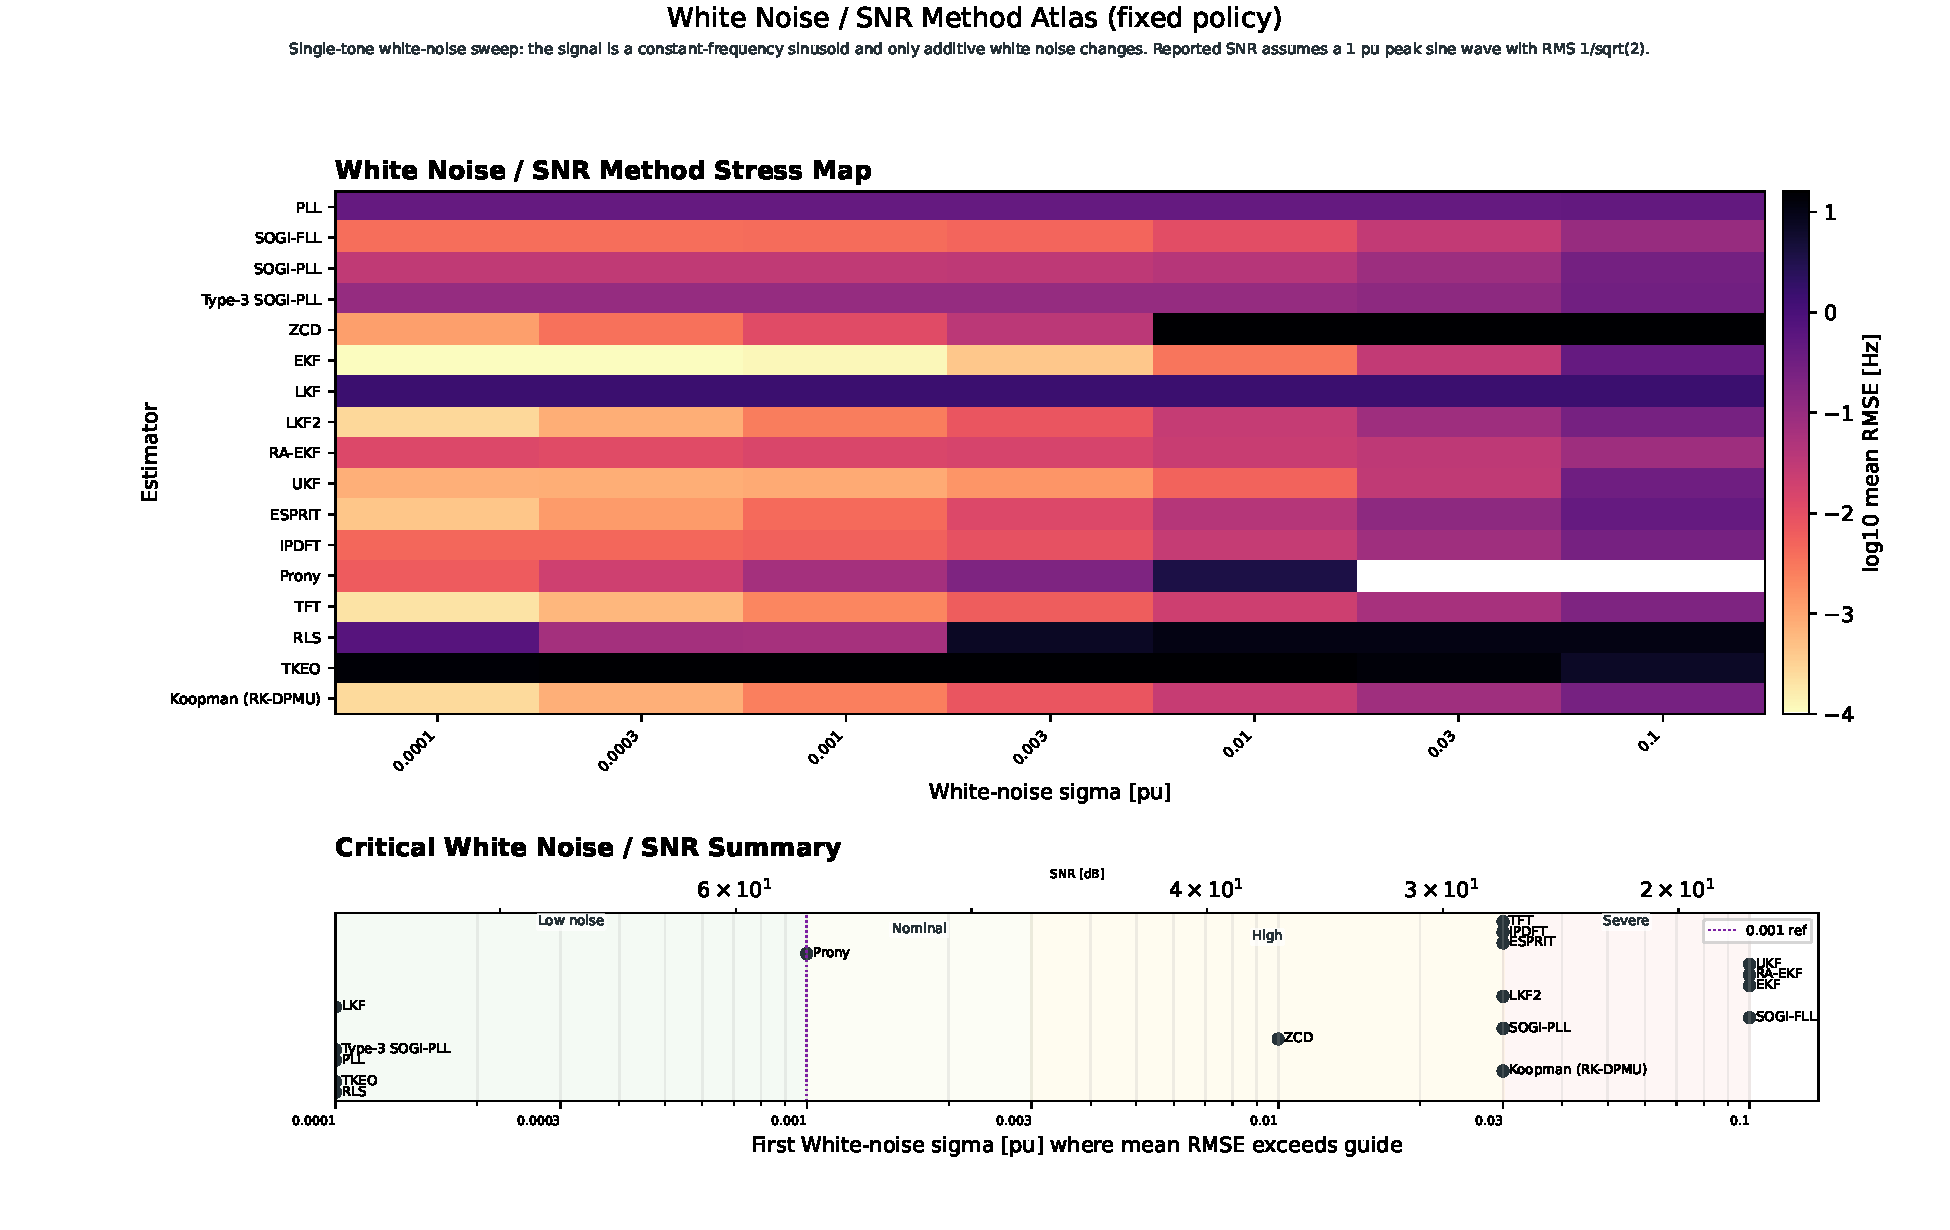
\includegraphics[width=\linewidth,height=0.66\textheight,keepaspectratio]{figures/noise_snr_method_map.pdf}
\end{columns}
\callout{Aggregate rankings hide stress-specific collapse: the same estimator is the best and the worst depending on the disturbance. The benchmark reports per-stress behavior, not one score.}
\end{frame}

\begin{frame}{Harmonic degradation differs by estimator family}
\atlaspreviewbanner
\begin{columns}[T,onlytextwidth]
\column{0.66\linewidth}
\centering
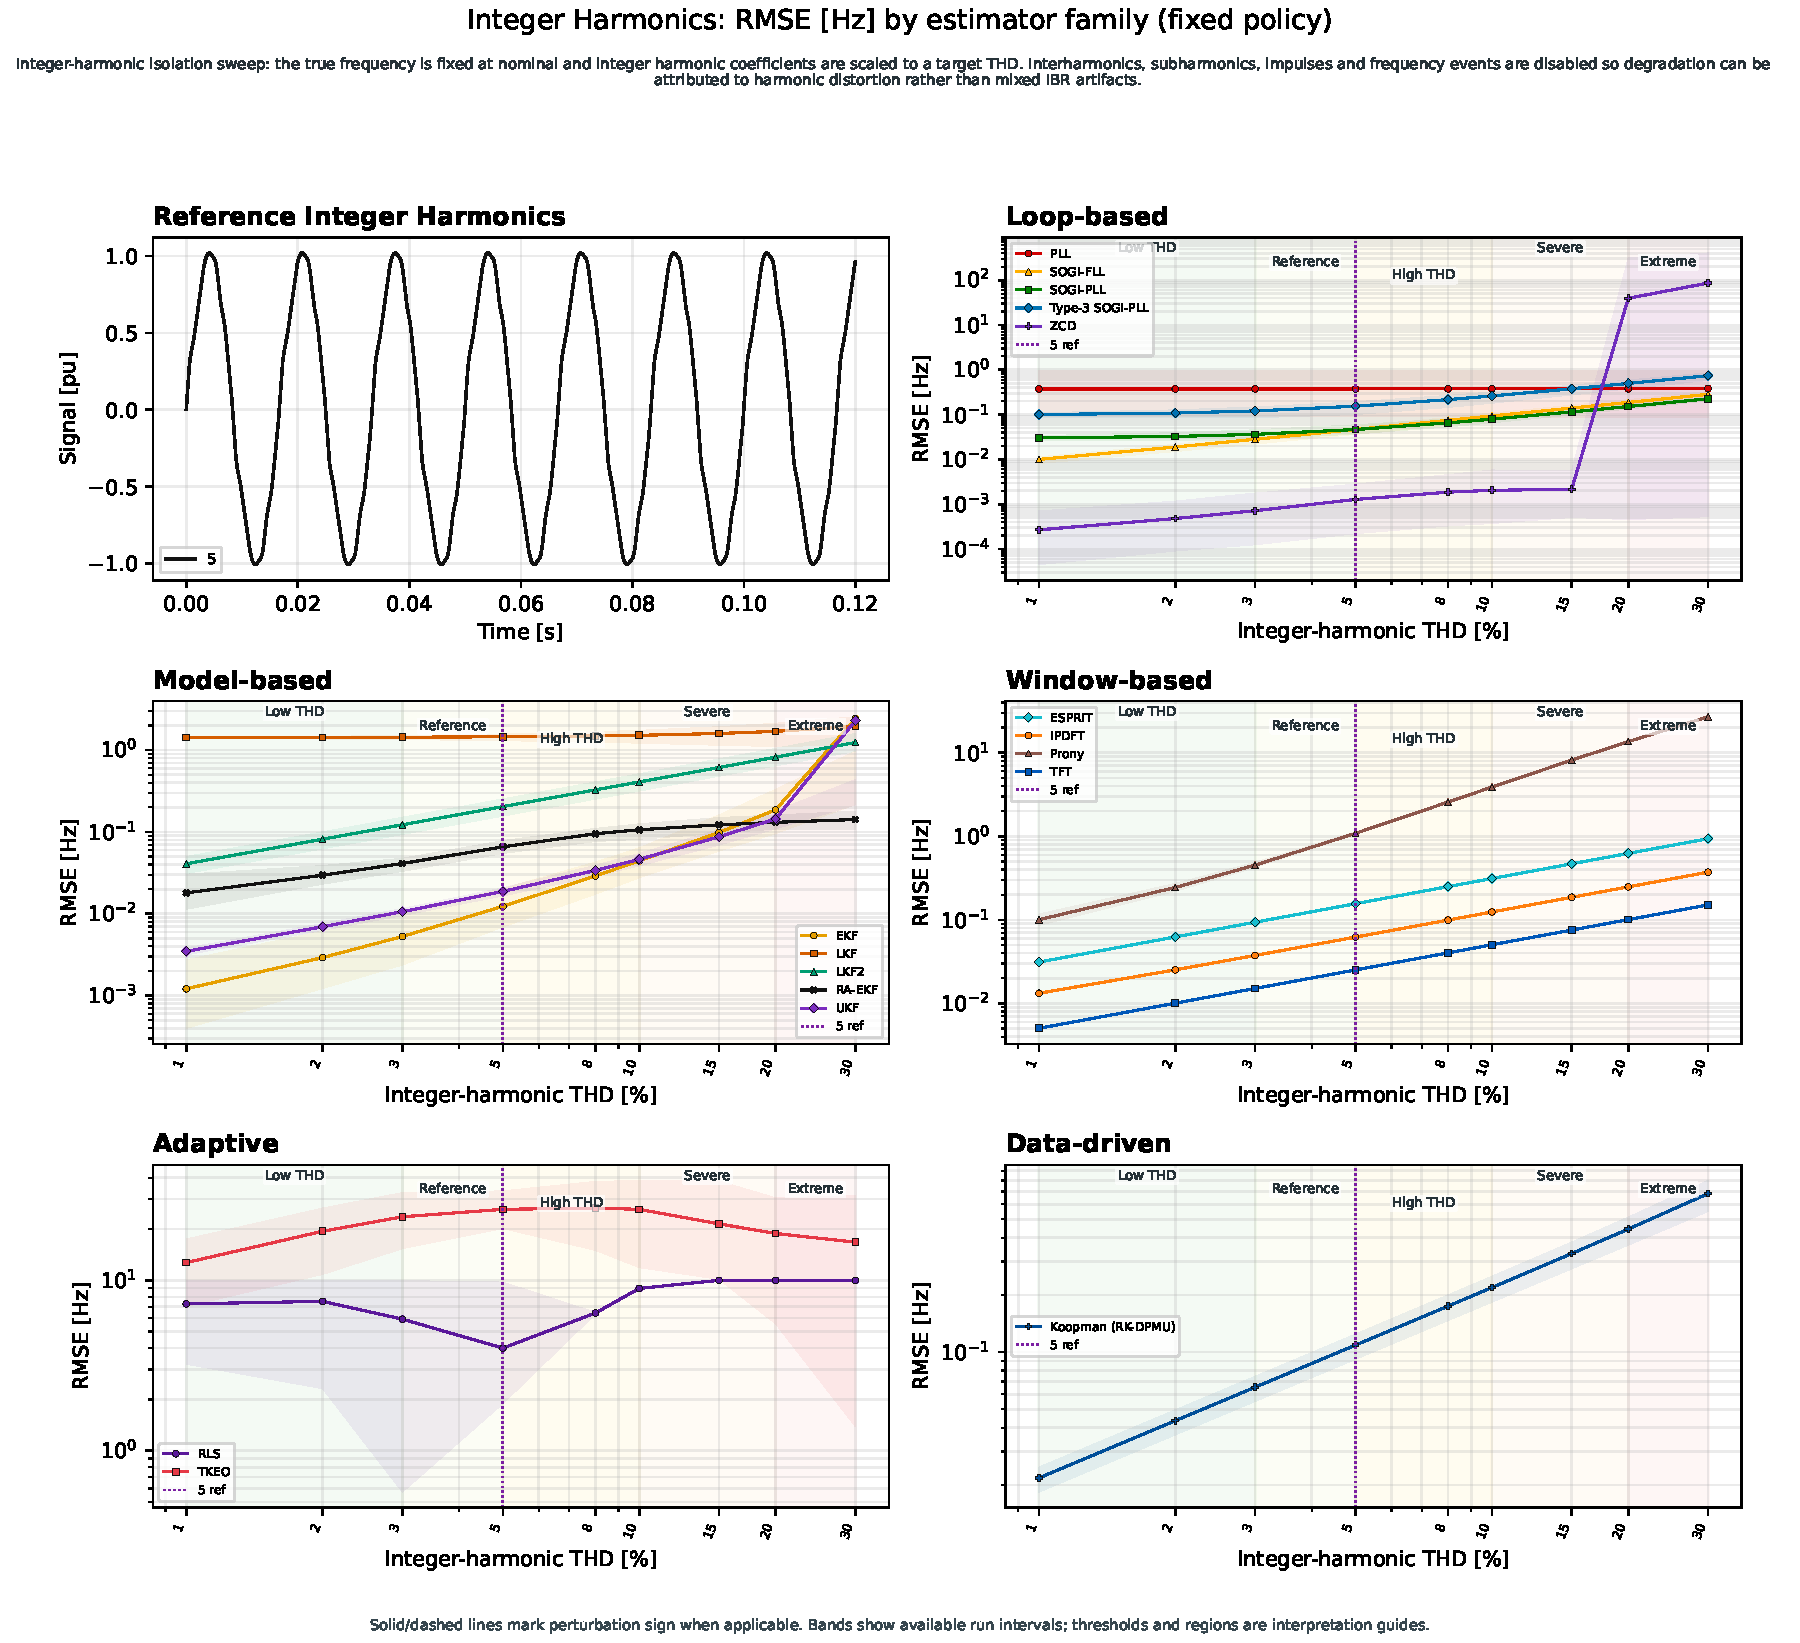
\includegraphics[width=\linewidth,height=0.70\textheight,keepaspectratio]{figures/harmonics_family_deterioration.pdf}
\column{0.30\linewidth}
\begin{block}{Reading}
\scriptsize
\begin{itemize}
  \item Loop, window, model, and adaptive families degrade with THD at different rates.
  \item Best low-THD accuracy does not predict high-THD survival.
  \item Window methods hold up; some adaptive/model methods degrade steeply.
\end{itemize}
\end{block}
\end{columns}
\end{frame}

\begin{frame}{RoCoF has a sign: down-ramps are harder}
\diagbanner
\begin{columns}[T,onlytextwidth]
\column{0.56\linewidth}
\centering
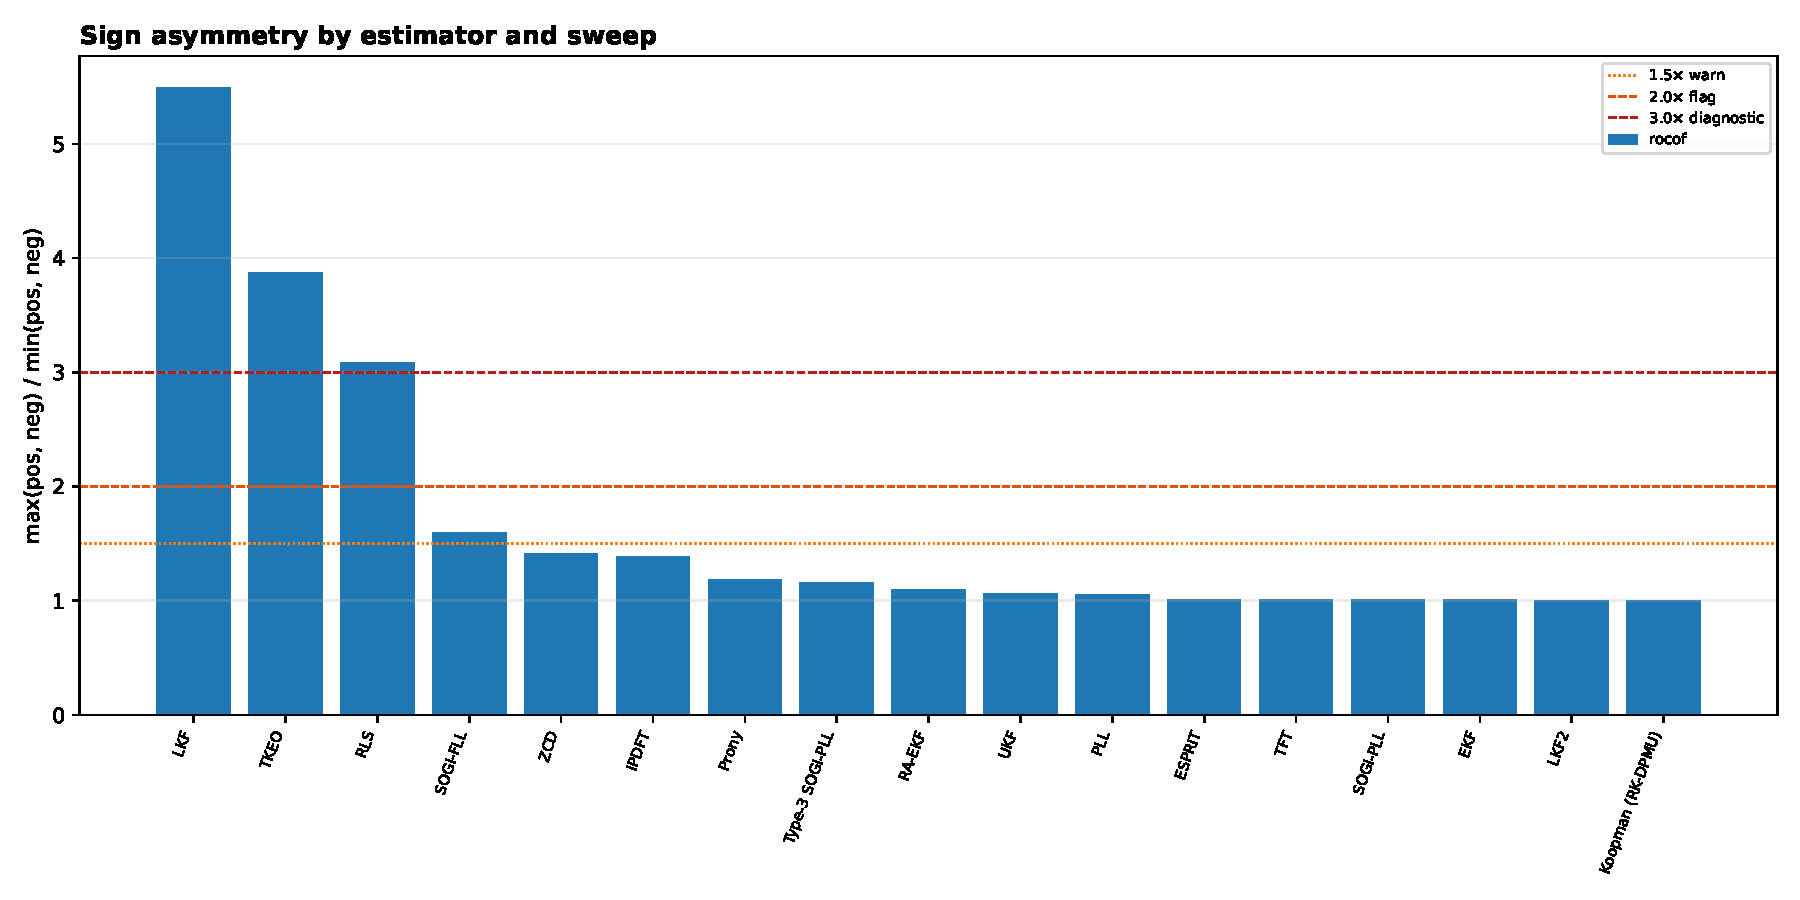
\includegraphics[width=\linewidth,height=0.68\textheight,keepaspectratio]{figures/rocof_sign_asymmetry.pdf}
\column{0.40\linewidth}
\scriptsize
\begin{block}{Directional bias (RMSE$_-$/RMSE$_+$ at $\pm$50 Hz/s)}
\begin{itemize}
  \item LKF \textbf{5.5$\times$} worse on $-$RoCoF
  \item TKEO \textbf{3.9$\times$}, RLS \textbf{3.0$\times$}
  \item SOGI-FLL 1.6$\times$
  \item EKF, UKF, RA-EKF $\approx$\,1.0 (symmetric)
\end{itemize}
\end{block}
\begin{block}{Why it matters}
A $+$RoCoF-only test can certify a method that fails on frequency \emph{decline} --- the protection-critical direction. Both signs must be swept.
\end{block}
\end{columns}
\artifact{atlas-rocof-diag-v1/atlas\_sign\_asymmetry.csv}
\end{frame}

\begin{frame}{Phase-jump severity is non-monotone}
\atlaspreviewbanner
\begin{columns}[T,onlytextwidth]
\column{0.58\linewidth}
\centering
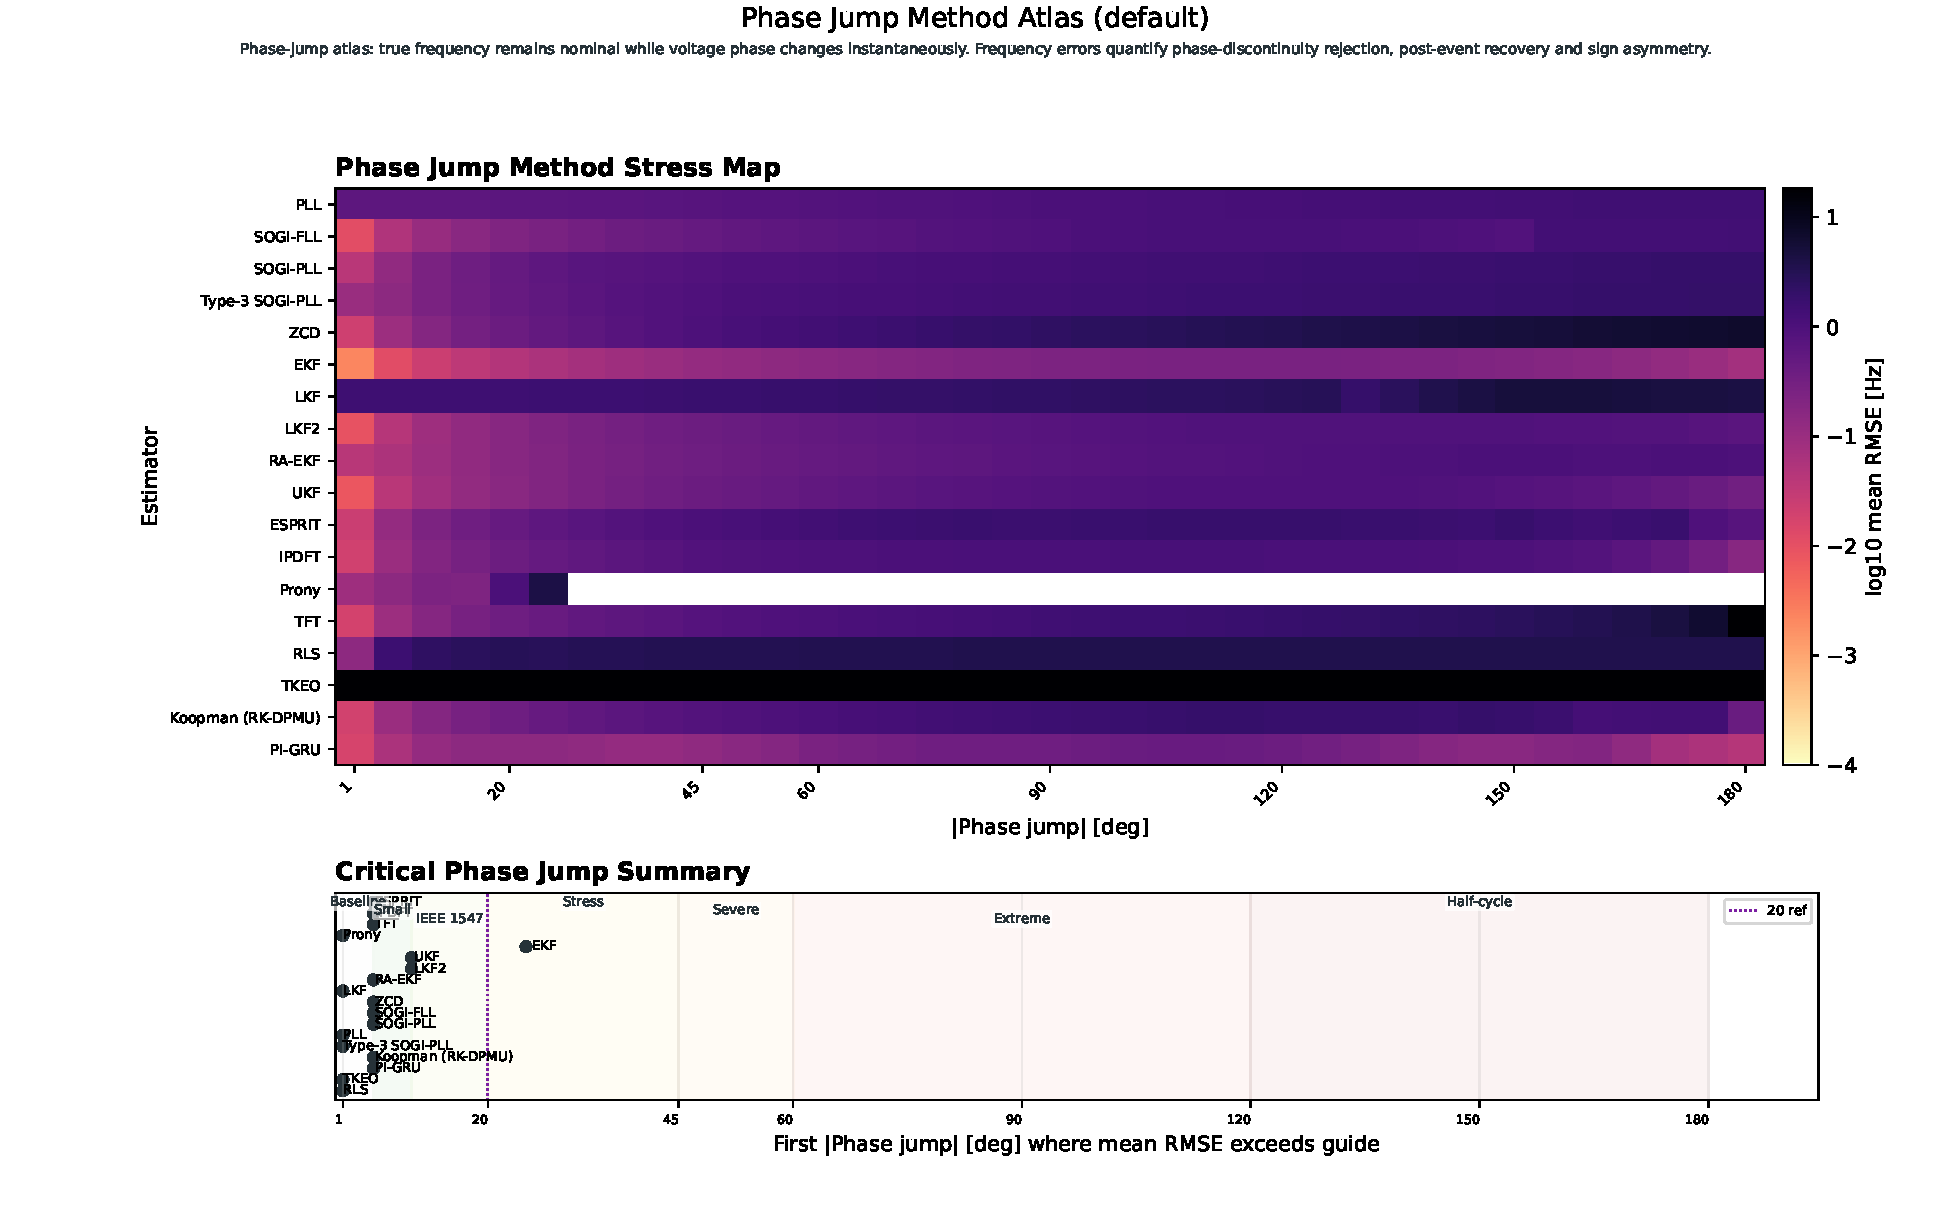
\includegraphics[width=\linewidth,height=0.60\textheight,keepaspectratio]{figures/phase_jump_method_map.pdf}
\column{0.38\linewidth}
\scriptsize
\begin{block}{Worst case is not 180$^\circ$}
Most methods peak near 90--120$^\circ$ and \emph{recover} toward 180$^\circ$ (a half-cycle jump partly self-cancels). EKF peaks at only \textbf{0.25 Hz @\,115$^\circ$}, back to 0.07 Hz @\,180$^\circ$.
\end{block}
\begin{block}{The TFT cliff}
One exception: TFT rises gently, then jumps \textbf{2.5\,$\rightarrow$\,21.9 Hz} between 150$^\circ$ and 180$^\circ$ --- a phase-reversal singularity.
\end{block}
\end{columns}
\callout{``Bigger jump = worse'' is wrong for this family. Severity sweeps, not single test points, expose where each estimator actually breaks.}
\end{frame}

\begin{frame}{No universal winner: champions rotate by regime}
\diagbanner
\begin{columns}[T,onlytextwidth]
\column{0.46\linewidth}
\scriptsize
\setlength{\tabcolsep}{4pt}
\renewcommand{\arraystretch}{1.28}
\begin{tabular}{>{\raggedright\arraybackslash}p{0.46\linewidth}>{\raggedright\arraybackslash}p{0.27\linewidth}r}
\toprule
RoCoF regime & Best & med.\ RMSE \\
\midrule
Low (0.1--1 Hz/s) & Koopman & 4.2 mHz \\
Standard (1--3) & ESPRIT & 7.8 mHz \\
IBR stress (3--10) & ESPRIT & 22.4 mHz \\
Severe (10--30) & SOGI-PLL & 70.3 mHz \\
\bottomrule
\end{tabular}
\vspace{0.35em}
\begin{block}{Across stress types}
EKF wins small phase jumps; ZCD wins harmonics-only; RA-EKF wins ramps and the step; UKF/EKF lead RoCoF-error. No method leads everywhere.
\end{block}
\column{0.50\linewidth}
\centering
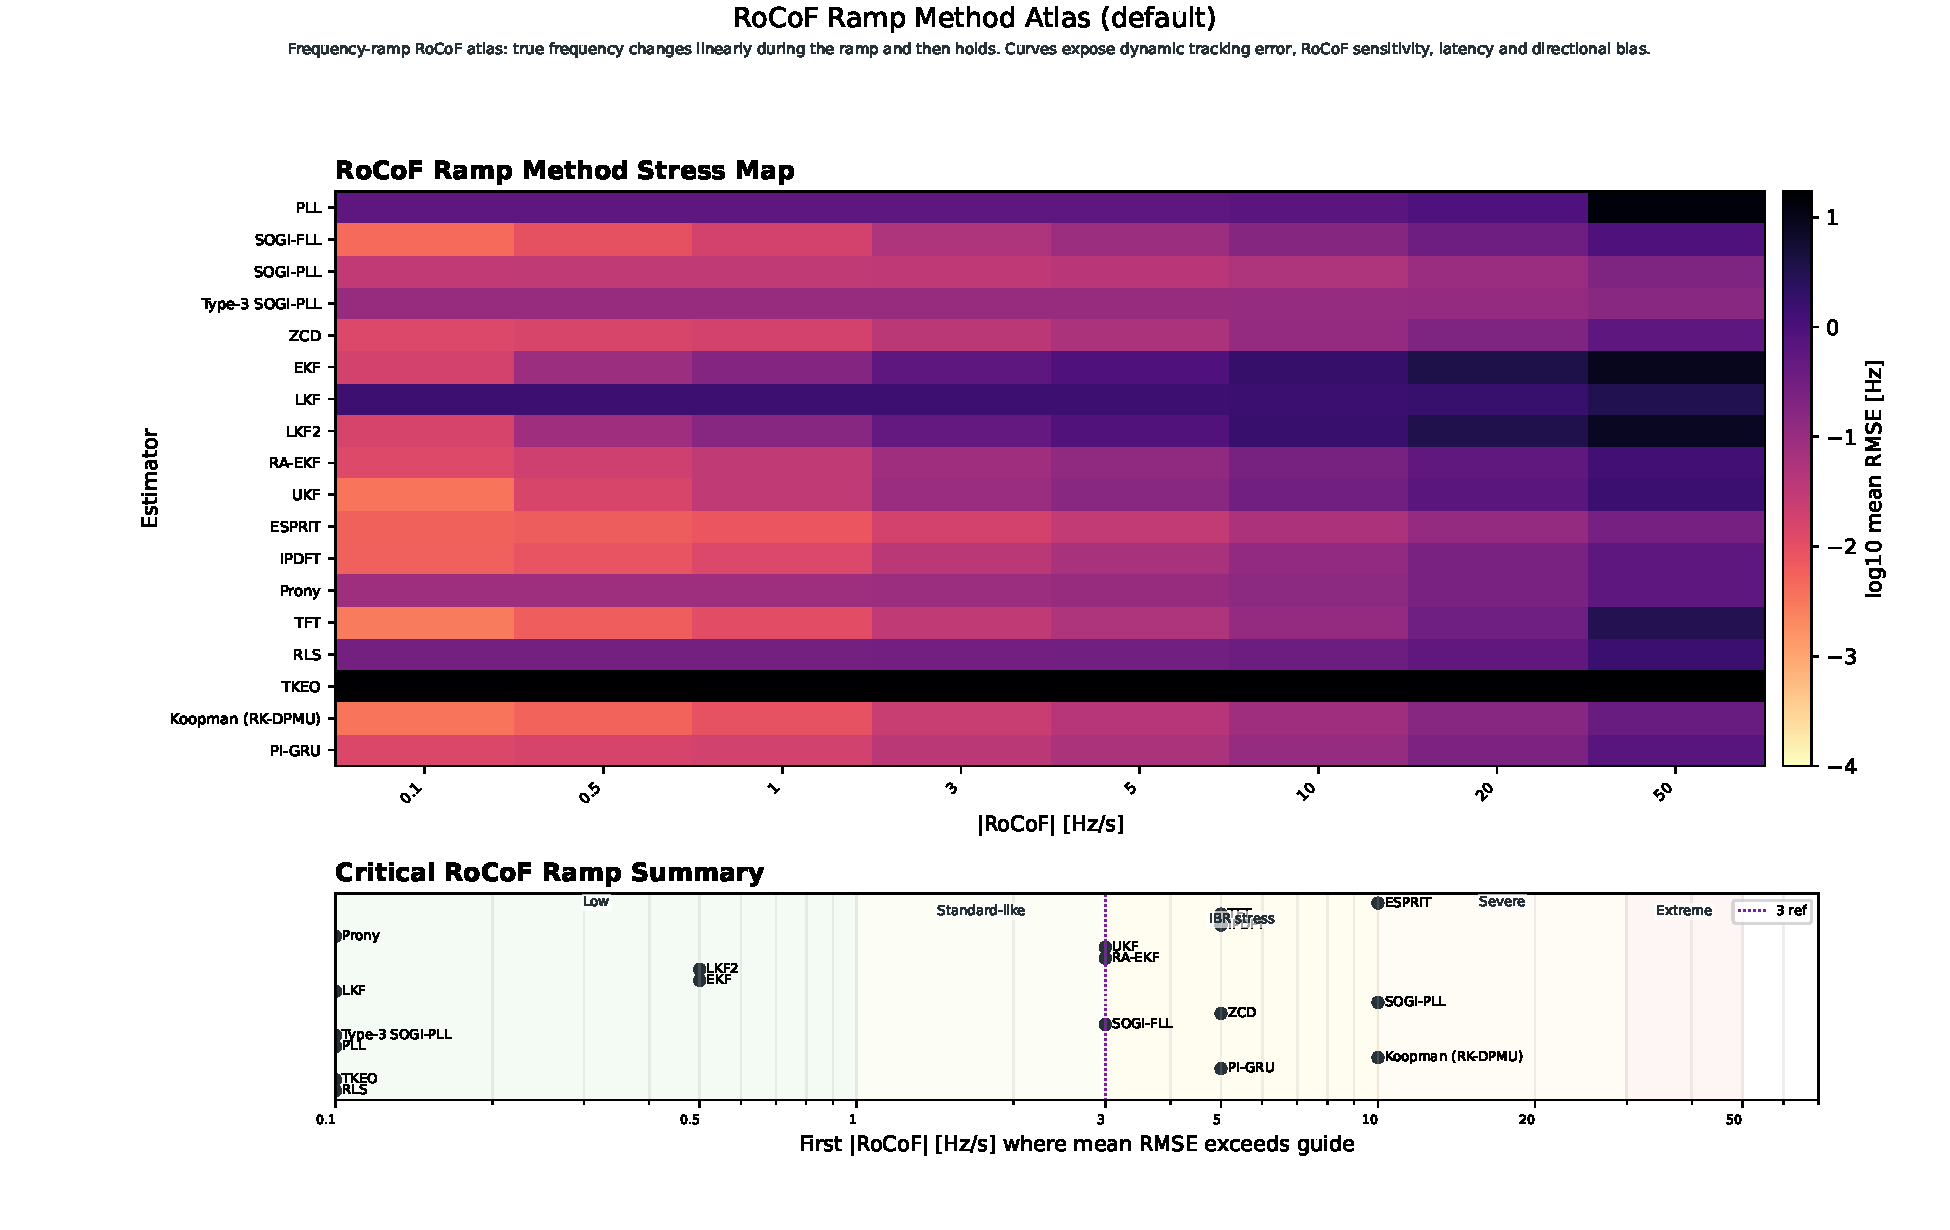
\includegraphics[width=\linewidth,height=0.68\textheight,keepaspectratio]{figures/rocof_method_map.pdf}
\end{columns}
\callout{The deliverable is a selection map --- event class $\times$ metric $\times$ compute budget --- not a single ranking.}
\end{frame}

\begin{frame}{Three findings}
\begin{enumerate}
  \item \textbf{Latency and stress trade-off}: IpDFT/TFT provide strong steady-state accuracy but carry 3--5 cycle structural delay; loop methods are fast but can suffer elevated trip exposure.
  \item \textbf{State-space estimation matters}: RA-EKF's explicit $\dot\omega$ state plus event gating reduces Scenario-D trip exposure from 0.165 s for EKF to about 0.6 ms.
  \item \textbf{Compliance tests are insufficient}: estimators that pass standard-style Step/Ramp/Mod cases can fail under composite islanding and multi-event IBR stress.
\end{enumerate}
\vspace{0.4em}
\callout{Estimator qualification includes transient recovery, trip exposure, compute feasibility, and standard-case RMSE.}
\end{frame}

\begin{frame}{Validity limits and next steps}
\begin{columns}[T,onlytextwidth]
\column{0.48\linewidth}
\begin{block}{Validation limits}
\small
\begin{itemize}
  \item Limited to the reported scenario set.
  \item CPU is a software-level cost indicator; hardware latency requires platform timing.
  \item The study is simulation-only.
  \item Scenario-wise tuning can affect rank stability.
\end{itemize}
\end{block}
\column{0.47\linewidth}
\begin{block}{Validation program}
\small
\begin{itemize}
  \item Hardware-in-the-loop validation.
  \item Wider converter-control interaction coverage.
  \item Sensitivity analysis of the tuning protocol.
  \item ATLAS severity and sign sweeps with validation gates.
\end{itemize}
\end{block}
\end{columns}
\vspace{0.35em}
\callout{These limits define the validation path: broader event coverage, hardware timing, fixed-policy replication, and field replay.}
\end{frame}

\ifbackupframes
\begin{frame}{Methodological findings}
\begin{enumerate}
  \item Disturbance family changes the estimator ranking and must be the first axis of interpretation.
  \item RMSE, peak error, trip-risk duration, and settling time should be evaluated as separate objectives.
  \item Latency and CPU cost are scientific response variables for deployability.
  \item Composite IBR stress is necessary because isolated compliance-style cases hide mixed-event failure modes.
  \item ATLAS validation gates prevent pilot sweeps from being interpreted as final qualification evidence.
\end{enumerate}
\vspace{0.4em}
\callout{Controlled traces, locked metrics, and artifact manifests make estimator comparisons reproducible.}
\end{frame}
\fi

\begin{frame}{Recommendation map}
\begin{center}
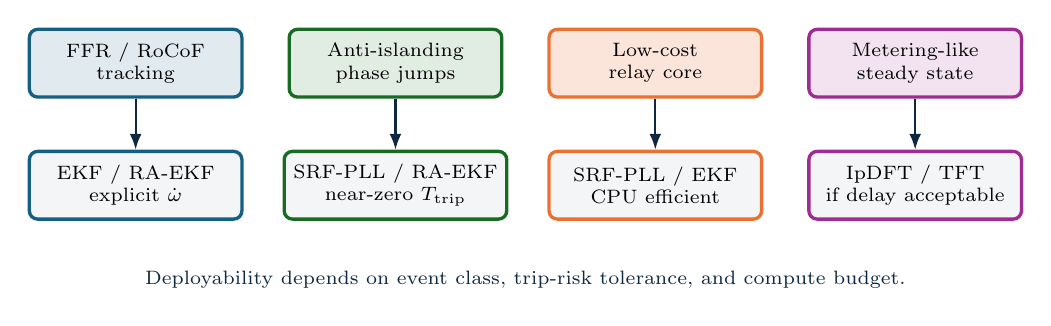
\begin{tikzpicture}[
  every node/.style={font=\scriptsize},
  task/.style={draw, rounded corners=3pt, minimum width=2.7cm, minimum height=0.86cm, align=center, very thick},
  arr/.style={-{Latex[length=2mm]}, thick, color=ofbInk}
]
\node[task, fill=ofbBlue!13, draw=ofbBlue] (monitor) at (0,1.2) {FFR / RoCoF\\tracking};
\node[task, fill=ofbGreen!13, draw=ofbGreen] (dyn) at (3.3,1.2) {Anti-islanding\\phase jumps};
\node[task, fill=ofbGold!18, draw=ofbGold] (rocof) at (6.6,1.2) {Low-cost\\relay core};
\node[task, fill=ofbViolet!13, draw=ofbViolet] (harm) at (9.9,1.2) {Metering-like\\steady state};
\node[task, fill=ofbSoft, draw=ofbBlue] (m1) at (0,-0.35) {EKF / RA-EKF\\explicit $\dot\omega$};
\node[task, fill=ofbSoft, draw=ofbGreen] (m2) at (3.3,-0.35) {SRF-PLL / RA-EKF\\near-zero $T_{\mathrm{trip}}$};
\node[task, fill=ofbSoft, draw=ofbGold] (m3) at (6.6,-0.35) {SRF-PLL / EKF\\CPU efficient};
\node[task, fill=ofbSoft, draw=ofbViolet] (m4) at (9.9,-0.35) {IpDFT / TFT\\if delay acceptable};
\draw[arr] (monitor) -- (m1);
\draw[arr] (dyn) -- (m2);
\draw[arr] (rocof) -- (m3);
\draw[arr] (harm) -- (m4);
\node[align=center, ofbInk] at (4.95,-1.55) {Deployability depends on event class, trip-risk tolerance, and compute budget.};
\end{tikzpicture}
\end{center}
\end{frame}

\ifbackupframes
\begin{frame}{Four results}
\begin{itemize}
  \item \textbf{RA-EKF targets phase-jump recovery}: explicit $\dot\omega$, covariance scaling, and event gating reduce false-trip exposure.
  \item \textbf{Trip-risk separates from RMSE}: Scenario D and E show why cumulative time outside a protection band must be reported separately.
  \item \textbf{CPU changes the answer}: SRF-PLL and EKF remain strong low-cost references; PI-GRU falls outside protection-real-time in the reported baseline.
  \item \textbf{ATLAS expands the stress space}: severity, sign, policy, latency, and reproducibility analyses explain ranking stability.
\end{itemize}
\end{frame}
\fi


\begin{frame}{Qualification profile}
\begin{center}
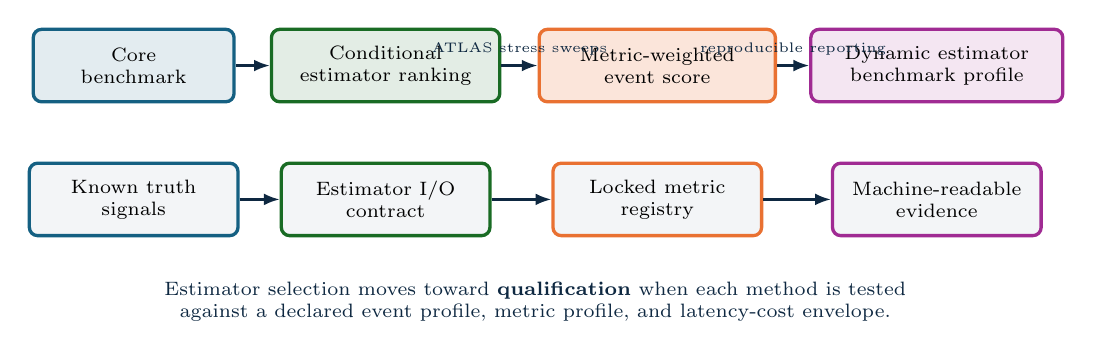
\begin{tikzpicture}[
  every node/.style={font=\scriptsize},
  box/.style={draw, rounded corners=3pt, minimum height=0.92cm, align=center, very thick},
  arr/.style={-{Latex[length=2mm]}, thick, color=ofbInk}
]
\node[box, fill=ofbBlue!12, draw=ofbBlue, minimum width=2.55cm] (paper) at (0,1.25) {Core\\benchmark};
\node[box, fill=ofbGreen!12, draw=ofbGreen, minimum width=2.9cm] (result) at (3.2,1.25) {Conditional\\estimator ranking};
\node[box, fill=ofbGold!18, draw=ofbGold, minimum width=3.0cm] (metric) at (6.65,1.25) {Metric-weighted\\event score};
\node[box, fill=ofbViolet!12, draw=ofbViolet, minimum width=3.2cm] (profile) at (10.2,1.25) {Dynamic estimator\\benchmark profile};
\draw[arr] (paper) -- (result);
\draw[arr] (result) -- node[above, font=\tiny] {ATLAS stress sweeps} (metric);
\draw[arr] (metric) -- node[above, font=\tiny] {reproducible reporting} (profile);
\node[box, fill=ofbSoft, draw=ofbBlue, minimum width=2.65cm] (s1) at (0,-0.45) {Known truth\\signals};
\node[box, fill=ofbSoft, draw=ofbGreen, minimum width=2.65cm] (s2) at (3.2,-0.45) {Estimator I/O\\contract};
\node[box, fill=ofbSoft, draw=ofbGold, minimum width=2.65cm] (s3) at (6.65,-0.45) {Locked metric\\registry};
\node[box, fill=ofbSoft, draw=ofbViolet, minimum width=2.65cm] (s4) at (10.2,-0.45) {Machine-readable\\evidence};
\draw[arr] (s1) -- (s2);
\draw[arr] (s2) -- (s3);
\draw[arr] (s3) -- (s4);
\node[align=center, text width=10.8cm, color=ofbInk] at (5.1,-1.75) {
Estimator selection moves toward \textbf{qualification} when each method is tested against a declared event profile, metric profile, and latency-cost envelope.
};
\end{tikzpicture}
\end{center}
\end{frame}

\begin{frame}{Standardization profile}
\begin{columns}[T,onlytextwidth]
\column{0.48\linewidth}
\begin{block}{Current standardization layer}
\scriptsize
\begin{itemize}
  \item PMU standards define phasor, frequency, and RoCoF measurement requirements.
  \item Compliance tests are necessary, with estimator-family ranking by IBR event survival left outside scope.
  \item Device reports often hide algorithmic failure modes behind aggregate accuracy.
\end{itemize}
\end{block}
\begin{block}{Standardization boundary}
\scriptsize
A dynamic-estimator profile needs declared signals, estimator I/O, metrics, evidence artifacts, and latency-cost reporting.
\end{block}
\column{0.47\linewidth}
\begin{block}{Benchmark profile}
\scriptsize
\begin{itemize}
  \item Canonical events: steps, ramps, phase jumps, ringdown, harmonics, interharmonics, noise, and composite IBR sequences.
  \item Locked metrics: RMSE, peak error, RoCoF error, trip-risk, settling, invalid samples, CPU, and latency.
  \item Task profiles: forensic monitoring, PMU augmentation, DFR support, and relay-adjacent screening.
\end{itemize}
\end{block}
\begin{block}{Standardization value}
\scriptsize
A reference test profile needs the same signals, estimator I/O, metrics, and machine-readable evidence.
\end{block}
\end{columns}
\end{frame}

\begin{frame}{IBR Event Qualification Score}
\readinessmetricbanner
\begin{columns}[T,onlytextwidth]
\column{0.53\linewidth}
\begin{block}{Score for estimator $e$}
\scriptsize
\begin{center}
\resizebox{0.98\linewidth}{!}{$
\begin{aligned}
\mathrm{IBR\text{-}ERS}(e) &= 1-\sum_{s\in\mathcal{S}} w_s\,\Phi_s(e),\\
\Phi_s(e) &= \alpha \tilde E_s+\beta \tilde P_s+\gamma \tilde T_s+\delta \tilde S_s+\eta \tilde C_s+\lambda \tilde L_s .
\end{aligned}
$}
\end{center}
\end{block}
\begin{itemize}
  \item $\tilde E_s$: normalized dynamic RMSE.
  \item $\tilde P_s$: normalized peak deviation.
  \item $\tilde T_s$: trip-risk duration.
  \item $\tilde S_s$: settling and recovery penalty.
  \item $\tilde C_s,\tilde L_s$: compute and latency penalties.
\end{itemize}
\column{0.43\linewidth}
\begin{block}{Composite metric}
\small
RMSE, trip-risk, transient recovery, and cost lead to different decisions. A composite score states the deployment objective explicitly.
\end{block}
\begin{block}{Profile-specific weights}
\small
Protection-adjacent use can raise $\gamma,\delta,\lambda$; forensic reconstruction can raise $\alpha,\beta$; embedded monitoring can raise $\eta$.
\end{block}
\end{columns}
\end{frame}

\begin{frame}{Toward realtime IBR estimators}
\begin{center}
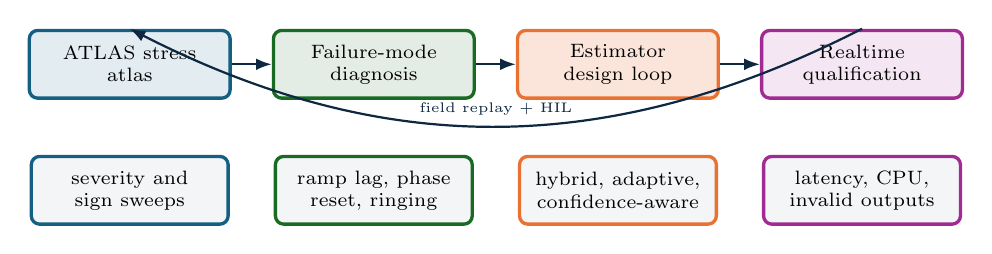
\begin{tikzpicture}[
  every node/.style={font=\scriptsize},
  box/.style={draw, rounded corners=3pt, minimum width=2.55cm, minimum height=0.86cm, align=center, very thick},
  arr/.style={-{Latex[length=2mm]}, thick, color=ofbInk}
]
\node[box, fill=ofbBlue!12, draw=ofbBlue] (atlas) at (0,0.85) {ATLAS stress\\atlas};
\node[box, fill=ofbGreen!12, draw=ofbGreen] (diag) at (3.1,0.85) {Failure-mode\\diagnosis};
\node[box, fill=ofbGold!18, draw=ofbGold] (design) at (6.2,0.85) {Estimator\\design loop};
\node[box, fill=ofbViolet!12, draw=ofbViolet] (deploy) at (9.3,0.85) {Realtime\\qualification};
\draw[arr] (atlas) -- (diag);
\draw[arr] (diag) -- (design);
\draw[arr] (design) -- (deploy);
\draw[arr, bend left=27] (deploy.north) to node[above, font=\tiny] {field replay + HIL} (atlas.north);
\node[box, fill=ofbSoft, draw=ofbBlue, minimum width=2.5cm] at (0,-0.75) {severity and\\sign sweeps};
\node[box, fill=ofbSoft, draw=ofbGreen, minimum width=2.5cm] at (3.1,-0.75) {ramp lag, phase\\reset, ringing};
\node[box, fill=ofbSoft, draw=ofbGold, minimum width=2.5cm] at (6.2,-0.75) {hybrid, adaptive,\\confidence-aware};
\node[box, fill=ofbSoft, draw=ofbViolet, minimum width=2.5cm] at (9.3,-0.75) {latency, CPU,\\invalid outputs};
\end{tikzpicture}
\end{center}
\vspace{0.35em}
\begin{itemize}
  \item The stress analysis identifies which physical stressor breaks each estimator family.
  \item That diagnosis supports hybrid estimators: event classifiers, harmonic-aware preprocessing, adaptive bandwidth, and self-reported confidence.
  \item Validation should combine synthetic truth, EMT replay, hardware-in-the-loop, and field oscillography.
\end{itemize}
\end{frame}

\begin{frame}{Conclusion and validation agenda}
\begin{columns}[T,onlytextwidth]
\column{0.49\linewidth}
\begin{block}{Conclusion}
\scriptsize
\begin{itemize}
  \item Field disturbances define the measurement problem; controlled synthetic truth makes estimator behavior explainable.
  \item The study compares estimators across objectives, regimes, and deployment constraints, including IBR-relevant stress modes.
  \item Empirical conclusions remain tied to evidence level, stress regime, and replication depth.
\end{itemize}
\end{block}
\column{0.49\linewidth}
\begin{block}{Validation agenda}
\scriptsize
\begin{itemize}
  \item Full ATLAS sweeps: fixed policy, 100-run Monte Carlo, statistical rank-stability analysis.
  \item Composite qualification profiles for forensic, PMU-augmentation, and relay-adjacent tasks.
  \item Three-phase, unbalance, and converter-control interaction coverage.
  \item Real-event replay from DFR/PMU/oscillography with synchronized ground-truth proxies.
  \item Estimators that optimize the full objective vector: frequency error, RoCoF, trip exposure, settling, CPU, latency.
\end{itemize}
\end{block}
\end{columns}
\vspace{0.30em}
\callout{\textbf{Result:} estimator choice is tied to the event class, metric target, and compute envelope; the next validation step evaluates each method against declared event regimes, latency limits, and compute envelopes.}
\end{frame}

\begin{frame}[plain]
\begin{tikzpicture}[remember picture,overlay]
  \node[anchor=center] at (current page.center) {\includegraphics[width=\paperwidth,height=\paperheight]{\sgsmaDividerBg}};
  \node[anchor=east, text=white, align=right, font=\fontsize{27}{32}\selectfont\rmfamily, text width=0.64\paperwidth] at ([xshift=-0.075\paperwidth,yshift=0.25cm]current page.east) {Backup};
  \node[anchor=east, text=white, align=right, font=\large, text width=0.62\paperwidth] at ([xshift=-0.075\paperwidth,yshift=-1.00cm]current page.east) {Metrics, extra stress maps, the planned paper-grade run, references.};
\end{tikzpicture}
\end{frame}

\begin{frame}{Backup: metric registry}
\scriptsize
\renewcommand{\arraystretch}{1.25}
\begin{tabular}{>{\bfseries}l >{\raggedright\arraybackslash}p{0.74\linewidth}}
\toprule
Metric & Definition \\
\midrule
M1 RMSE & $\sqrt{\mathrm{mean}\,e[k]^2}$ on steady-state-trimmed frequency error [Hz]. \\
M3 peak & $\max_k|e[k]|$ [Hz]. \\
M5 trip-risk & cumulative time with $|e[k]|>0.5$ Hz (protection-deadband risk proxy) [s]. \\
M6 max-contig trip & longest \emph{contiguous} deadband violation [s]. \\
M8 settling & time until $|e|$ stays $\le 0.2$ Hz [s]. \\
M9 / M10 RFE & RoCoF error: robust max (99.5th pct) / RMS of $|\widehat{\dot f}-\dot f|$ [Hz/s]. \\
M13 CPU & execution time per sample [$\mu$s] --- software-cost proxy, not hardware latency. \\
M14 latency & declared structural delay (window / group delay) [ms]. \\
M22 invalid rate & fraction of samples the estimator flags invalid / NaN. \\
\bottomrule
\end{tabular}
\vspace{0.3em}
\callout{Trip-risk is a protection-oriented risk proxy, not a relay trip command; CPU is a software-cost proxy. Differences below sampling/timing resolution are not interpreted.}
\artifact{src/analysis/metrics.py; docs/METHODS.md}
\end{frame}

\begin{frame}{Backup: frequency-step stress map}
\begin{center}
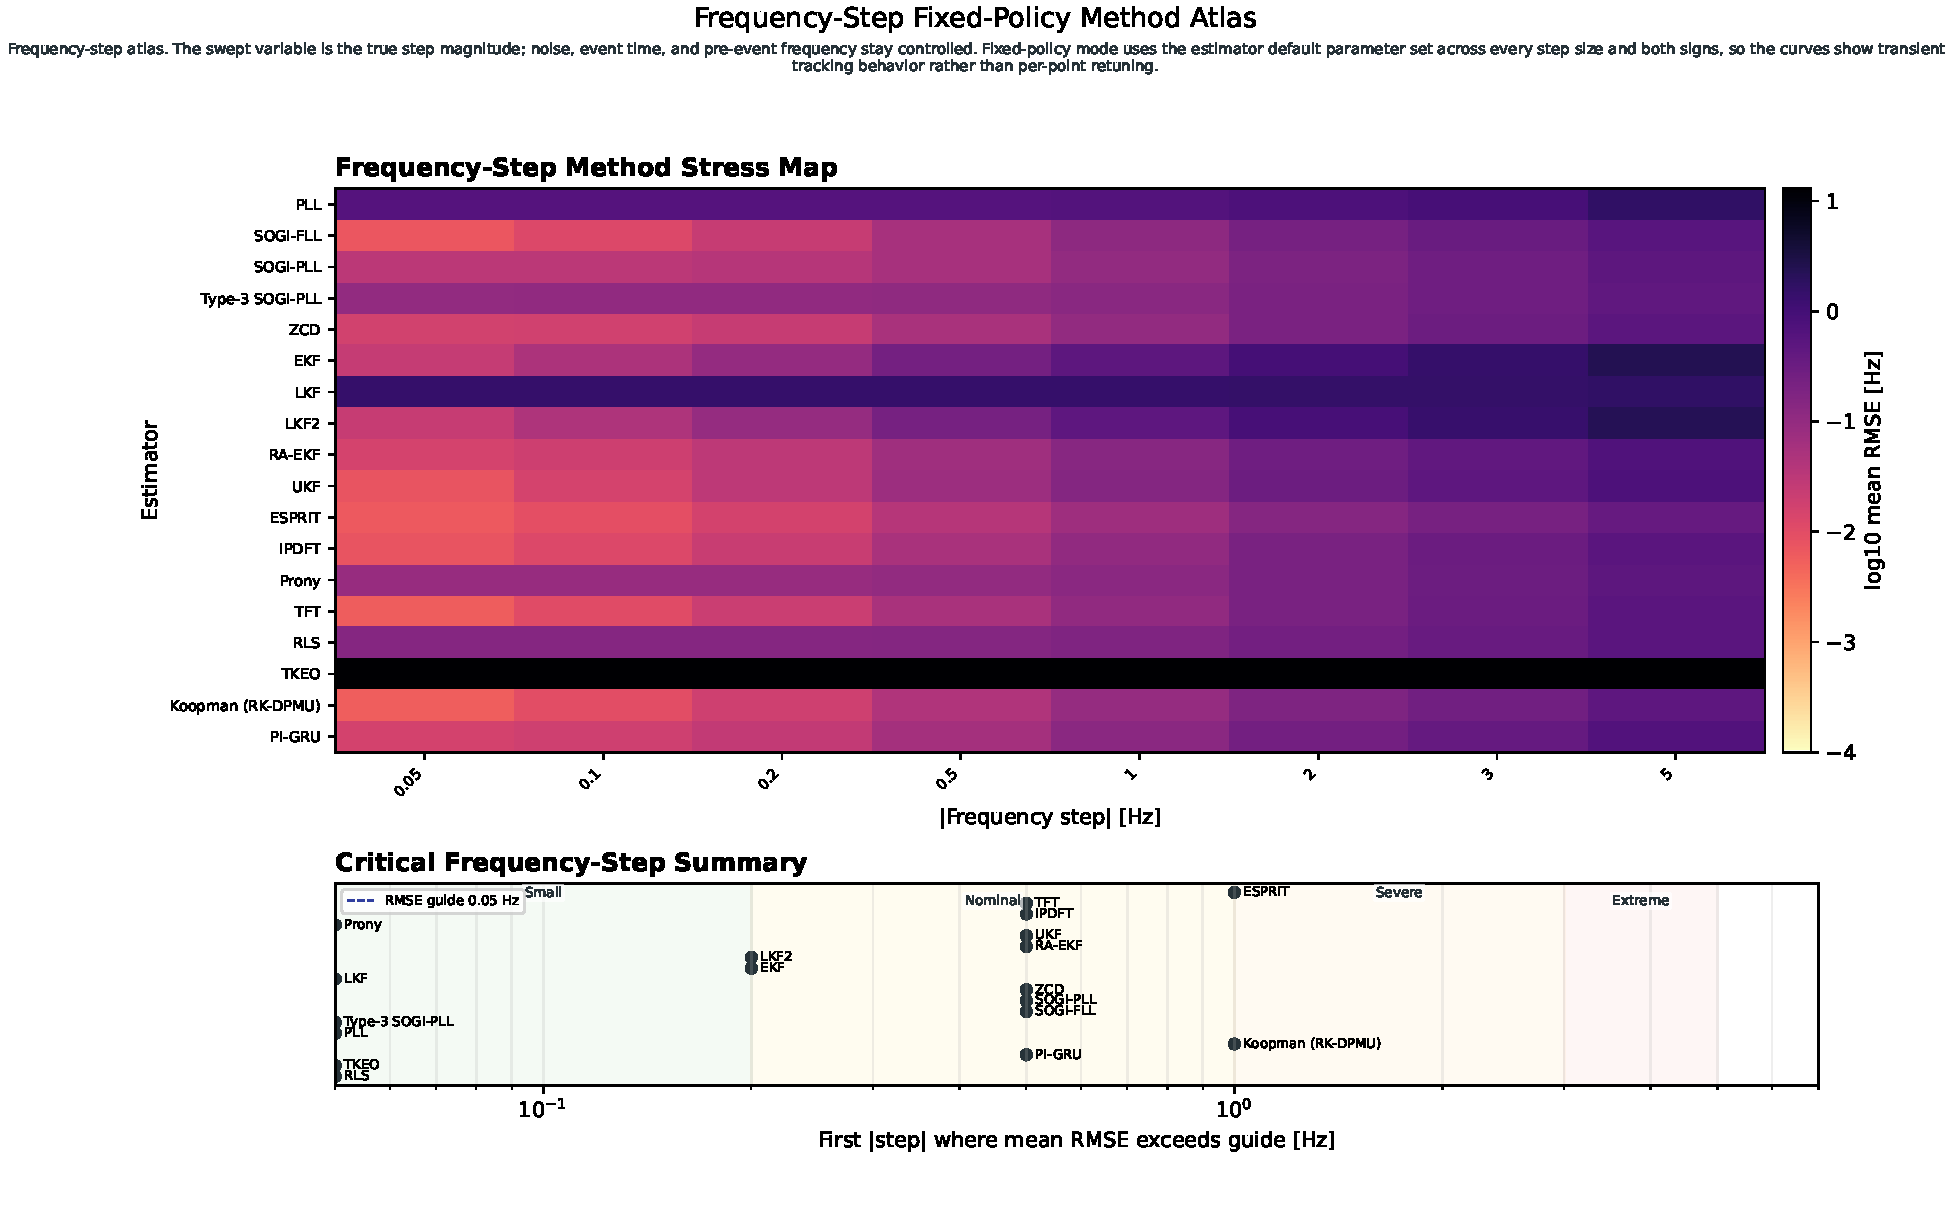
\includegraphics[width=0.94\linewidth,height=0.72\textheight,keepaspectratio]{figures/frequency_step_method_map.pdf}
\end{center}
\artifact{frequency\_step\_mvp2\_all18\_representative}
\end{frame}

\begin{frame}{Backup: noise robustness ranking}
\diagbanner
\begin{center}
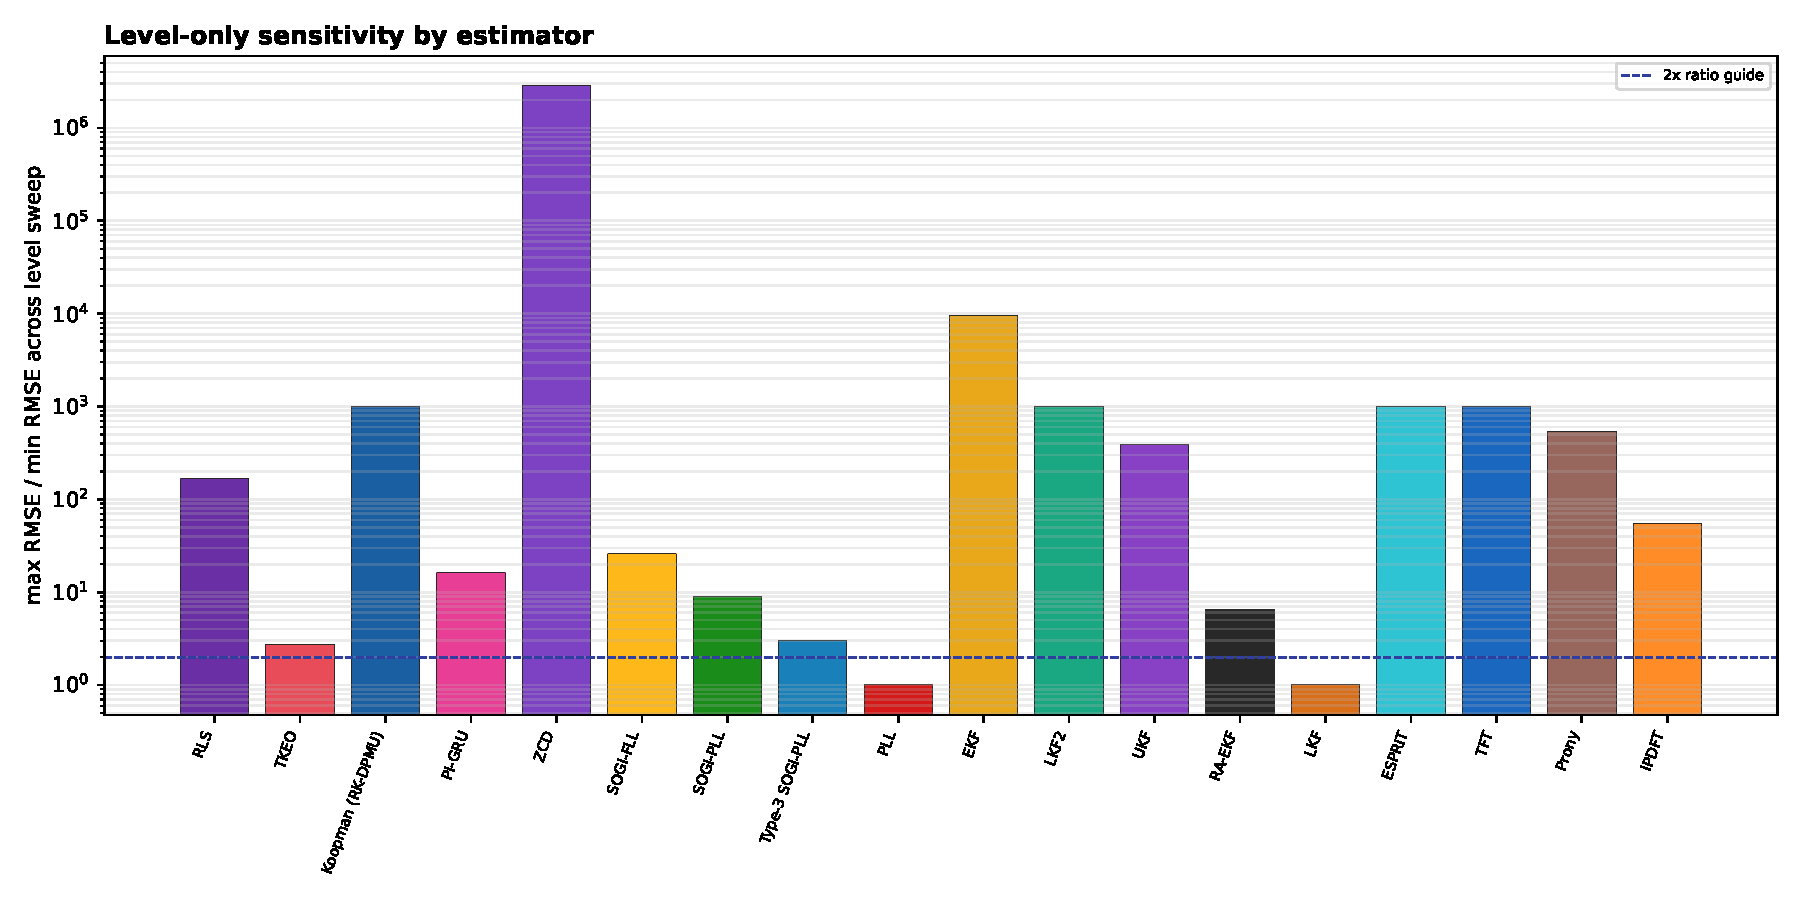
\includegraphics[width=0.92\linewidth,height=0.68\textheight,keepaspectratio]{figures/noise_snr_level_sensitivity.pdf}
\end{center}
\artifact{atlas-noise-snr-diag-v1}
\end{frame}

\begin{frame}{Backup: the paper-grade run (planned)}
\begin{columns}[T,onlytextwidth]
\column{0.54\linewidth}
\begin{block}{Target command}
\scriptsize
\texttt{python -m pipelines.atlas\_sweep --sweeps all --policy fixed\_policy --n-runs 100 --n-cost-reps 3 --tune-trials 80 --output-subdir atlas-full-v1}
\end{block}
\column{0.42\linewidth}
\scriptsize
\begin{itemize}
  \item Full 18-estimator canonical set, fixed policy.
  \item Both signs, $n\ge100$ Monte Carlo.
  \item Archived seeds, manifests, and hashes.
  \item Regenerate every table and figure from artifacts.
\end{itemize}
\end{columns}
\vspace{0.2em}
\callout{This converts today's diagnostic pilots into paper- and journal-grade claims through the readiness gate.}
\artifact{docs/ATLAS\_PIPELINE.md; docs/ATLAS\_ROADMAP.md}
\end{frame}

\begin{frame}{Backup: selected references}
\scriptsize
\begin{columns}[T,onlytextwidth]
\column{0.49\linewidth}
\textbf{Standards \& platforms}
\begin{itemize}
  \item IEEE/IEC 60255-118-1:2018 --- synchrophasor, frequency, RoCoF compliance.
  \item NISTIR 8106 --- PMU performance assessment.
  \item OpenPMU, openPDC, FNET/GridEye, LBNL micro-PMU, PNNL PMU event library.
\end{itemize}
\column{0.49\linewidth}
\textbf{IBR field events}
\begin{itemize}
  \item NERC Blue Cut Fire (2016), Canyon 2 (2017), Odessa (2021--22), CA BESS (2022).
  \item NERC IBR disturbance-monitoring white paper.
  \item Kaua'i 2021 18--20 Hz IBR oscillation analysis.
\end{itemize}
\end{columns}
\vspace{0.3em}
\callout{Field cases define the stress modes; no claim is made that a single estimator would have prevented a disturbance.}
\end{frame}

\ifbackupframes
\begin{frame}{Full-scale experimental protocol}
\begin{columns}[T,onlytextwidth]
\column{0.52\linewidth}
\begin{block}{Target command}
\small
\texttt{python -m pipelines.atlas\_sweep --sweeps all --policy fixed\_policy --n-runs 100 --n-cost-reps 3 --tune-trials 80 --output-subdir atlas-full-v1}
\end{block}
\column{0.42\linewidth}
\begin{itemize}
  \item Complete canonical estimator set.
  \item Full ATLAS sweep suite.
  \item Archived seeds, manifests, and hashes.
  \item Predefined hypotheses and figure scripts.
  \item Regenerate all tables from CSV/JSON artifacts.
\end{itemize}
\end{columns}
\artifact{docs/ATLAS\_PIPELINE.md}
\end{frame}
\fi

\ifbackupframes
\begin{frame}{Selected benchmark references}
\scriptsize
\begin{itemize}
  \item IEEE/IEC 60255-118-1:2018: synchrophasor, frequency, and RoCoF measurement definitions and compliance requirements.
  \item NISTIR 8106: NIST assessment of PMU performance against synchrophasor requirements.
  \item NIST PMU calibration service: traceable calibration of PMUs against IEEE synchrophasor standard requirements.
  \item OpenPMU: open-source PMU device/platform for phasor measurement research.
  \item openPDC: open-source phasor data concentrator for streaming synchrophasor infrastructure.
  \item FNET/GridEye: wide-area frequency disturbance recorder network for grid monitoring.
  \item LBNL Open micro-PMU datasets and PNNL open-source PMU event library: real event data for algorithm and application development.
  \item NERC recommended IBR disturbance monitoring: high-resolution DFR data, continuous PMU/DDR data, and inverter fault-code retention for post-mortem analysis.
\end{itemize}
\vspace{0.3em}
\callout{These references motivate the gap: standards and datasets leave room for controlled, estimator-level tests with known truth and deployability metrics.}
\end{frame}

\begin{frame}{Selected field-event references}
\scriptsize
\begin{itemize}
  \item NERC/WECC Blue Cut Fire report: 1,200 MW fault-induced solar PV resource interruption, Southern California, August 16, 2016.
  \item NERC/WECC Canyon 2 Fire report: 900 MW-class fault-induced solar PV resource interruption, Southern California, October 9, 2017.
  \item NERC Odessa disturbance reports: widespread solar PV reductions in Texas and associated model-fidelity and inverter-control findings.
  \item NERC 2022 California BESS disturbance report: abnormal BESS power reductions following normally cleared Western Interconnection faults.
  \item NERC Synchronized Measurements Subcommittee white paper on recommended disturbance monitoring for IBRs.
  \item Dong et al., Kaua'i 2021 18--20 Hz oscillation analysis: IBR-driven subsynchronous oscillation diagnosis and EMT replay.
  \item Ofgem/National Grid ESO 9 August 2019 GB outage reports and ENTSO-E 28 April 2025 Iberian incident report: grid-wide cascading events where fast dynamic visibility is central to diagnosis.
\end{itemize}
\vspace{0.25em}
\callout{The field cases define stress modes. No claim is made that a single estimator would have prevented a disturbance.}
\end{frame}

\appendix

\begin{frame}{Technical questions}
\scriptsize
\renewcommand{\arraystretch}{1.18}
\begin{tabular}{>{\bfseries\raggedright\arraybackslash}p{0.28\linewidth}>{\raggedright\arraybackslash}p{0.62\linewidth}}
\toprule
Question & Short answer \\
\midrule
Why scenario-wise tuning? & It estimates best-in-range behavior under the tested search space. Fixed-policy replication is the next qualification layer. \\
How is this different from IEC/IEEE compliance? & Compliance tests define device-level requirements. This study compares estimator algorithms under known truth, IBR-specific stress, trip-risk, and CPU cost. \\
Why Python CPU times? & CPU reports relative software cost. Embedded or FPGA timing requires implementation-specific replication. \\
What should be deployed? & For FFR and phase-jump anti-islanding, RA-EKF is the strongest benchmark-backed recommendation; SRF-PLL/EKF remain low-cost baselines; IpDFT/TFT are useful where observation delay is acceptable. \\
How reliable are ATLAS pilots? & They are pilot sweeps: $n=1$, default policy. Final qualification requires fixed policy, full estimator coverage, and replication. \\
Does this explain any blackout? & No. Field events define the stress modes; no prevention claim is made. \\
\bottomrule
\end{tabular}
\end{frame}

\begin{frame}{Artifact sources}
\scriptsize
\begin{itemize}
  \item \texttt{artifacts/frequency\_step\_mvp2\_all18\_representative/global\_metrics\_report.csv}
  \item \texttt{artifacts/frequency\_step\_mvp2\_all18\_representative/frequency\_step\_hypothesis\_tests.csv}
  \item \texttt{artifacts/freq\_ramp\_rocof\_mvp2\_all18\_representative/global\_metrics\_report.csv}
  \item \texttt{artifacts/freq\_ramp\_rocof\_mvp2\_all18\_representative/rocof\_hypothesis\_tests.csv}
  \item \texttt{artifacts/atlas-harmonics-fast14-preview-v2/global\_metrics\_report.csv}
  \item \texttt{artifacts/atlas-readiness-smoke/atlas\_readiness\_report.json}
  \item \texttt{slides/generate\_slide\_assets.py}
\end{itemize}
\end{frame}

\begin{frame}{Regeneration}
\begin{block}{Figures and tables}
\texttt{python slides\textbackslash generate\_slide\_assets.py}
\end{block}
\begin{block}{PDF}
\texttt{cd slides}\\
\texttt{pdflatex slide.tex}\\
\texttt{pdflatex slide.tex}
\end{block}
\end{frame}
\fi

\end{document}
